\documentclass[11pt]{scrartcl}
\usepackage[portuguese]{babel}
\usepackage[utf8]{inputenc}

\usepackage{nameref}
\usepackage[colorlinks=true, urlcolor=blue, citecolor=blue, linkcolor=blue]{hyperref}
\usepackage{amsfonts, amsmath, amssymb, amsthm, thmtools}
  
\usepackage{cleveref}

\declaretheorem[name=Teorema, refname={Teorema, Teoremas}, Refname={Teorema, Teoremas}, parent=section]{theorem}
\declaretheorem[name=Algoritmo, refname={Algoritmo, Algoritmos}, Refname={Algoritmo, Algoritmos}, sibling=theorem, style=definition]{algorithm2}
\declaretheorem[name=Corolário, refname={Corolário, Corolários}, Refname={Corolário, Corolários}, sibling=theorem]{corollary}
\declaretheorem[name=Definição, refname={Definição, Definições}, Refname={Definição, Definições}, sibling=theorem, style=definition]{definition}
\declaretheorem[name=Exemplo, refname={Exemplo, Exemplos}, Refname={Exemplo, Exemplos}, sibling=theorem, style=definition]{example}
\declaretheorem[name=Lema, refname={Lema, Lemas}, Refname={Lema, Lemas}, sibling=theorem]{lemma}
\declaretheorem[name=Exercício, refname={Exercício, Exercícios}, Refname={Exercício, Exercícios}, sibling=theorem, style=definition]{exercise}

\crefname{section}{seção}{seções}
\Crefname{section}{Seção}{Seções}
\crefname{table}{tabela}{tabelas}
\Crefname{table}{Tabela}{Tabelas}

\newcommand{\crefpairconjunction}{ e }
\newcommand{\creflastconjunction}{ e }

\usepackage{color, xcolor, enumitem, fancyhdr, float, layout, multirow, setspace, slashbox, verbatim}
\usepackage{algorithm2e, algorithmicx, listings}
\usepackage{caption, subcaption}
\usepackage[authoryear]{natbib}
\usepackage[all]{xy}
\usepackage{authblk}
\usepackage{cprotect}
\bibpunct[; ]{(}{)}{,}{a}{,}{;}

\usepackage{graphicx}
\graphicspath{{figures/}{../figures/}}
\renewcommand{\floatpagefraction}{.9}

\usepackage{ifthen}
\newboolean{noShowSolutions}
\newcommand{\solutioncmd}[2]{{{#1}}{{#2}}}
\newcommand{\solution}[2]{\ifthenelse {\boolean{noShowSolutions}} {\solutioncmd{#2}}{\solutioncmd{#1}}}
\usepackage{xcolor}
\def\X{***ATTN***}
\newcommand{\red}[1]{\textbf{\color{red} ***ATTN*** #1}}
\renewcommand{\vec}[1]{\mathbf{#1}}

\def\limn{\lim_{n \rightarrow \infty}}
\def\convas{\stackrel{a.s.}{\longrightarrow}}

\DeclareRobustCommand{\rchi}{{\mathpalette\irchi\relax}}
\newcommand{\irchi}[2]{\raisebox{\depth}{$#1\chi$}}

\def\I{{\mathbb I}}
\def\P{{\mathbb P}}
\def\E{{\mathbb E}}
\def\V{{\mathbb V}}
\def\N{{\mathbb N}}
\def\R{{\mathbb R}}
\def\seqn{{_{n \in N}}}
\def\X{{\vec{X}}}
\def\x{{\vec{x}}}
\def\Z{{\vec{Z}}}
\def\z{{\vec{z}}}

\makeatletter
\def\maxwidth{ %
  \ifdim\Gin@nat@width>\linewidth
    \linewidth
  \else
    \Gin@nat@width
  \fi
}
\makeatother

\definecolor{fgcolor}{rgb}{0.345, 0.345, 0.345}
\newcommand{\hlnum}[1]{\textcolor[rgb]{0.686,0.059,0.569}{#1}}%
\newcommand{\hlstr}[1]{\textcolor[rgb]{0.192,0.494,0.8}{#1}}%
\newcommand{\hlcom}[1]{\textcolor[rgb]{0.678,0.584,0.686}{\textit{#1}}}%
\newcommand{\hlopt}[1]{\textcolor[rgb]{0,0,0}{#1}}%
\newcommand{\hlstd}[1]{\textcolor[rgb]{0.345,0.345,0.345}{#1}}%
\newcommand{\hlkwa}[1]{\textcolor[rgb]{0.161,0.373,0.58}{\textbf{#1}}}%
\newcommand{\hlkwb}[1]{\textcolor[rgb]{0.69,0.353,0.396}{#1}}%
\newcommand{\hlkwc}[1]{\textcolor[rgb]{0.333,0.667,0.333}{#1}}%
\newcommand{\hlkwd}[1]{\textcolor[rgb]{0.737,0.353,0.396}{\textbf{#1}}}%

\usepackage{framed}
\makeatletter
\newenvironment{kframe}{%
 \def\at@end@of@kframe{}%
 \ifinner\ifhmode%
  \def\at@end@of@kframe{\end{minipage}}%
  \begin{minipage}{\columnwidth}%
 \fi\fi%
 \def\FrameCommand##1{\hskip\@totalleftmargin \hskip-\fboxsep
 \colorbox{shadecolor}{##1}\hskip-\fboxsep
     % There is no \\@totalrightmargin, so:
     \hskip-\linewidth \hskip-\@totalleftmargin \hskip\columnwidth}%
 \MakeFramed {\advance\hsize-\width
   \@totalleftmargin\z@ \linewidth\hsize
   \@setminipage}}%
 {\par\unskip\endMakeFramed%
 \at@end@of@kframe}
\makeatother

\definecolor{shadecolor}{rgb}{.97, .97, .97}
\definecolor{messagecolor}{rgb}{0, 0, 0}
\definecolor{warningcolor}{rgb}{1, 0, 1}
\definecolor{errorcolor}{rgb}{1, 0, 0}
\newenvironment{knitrout}{}{} % an empty environment to be redefined in TeX

\usepackage{alltt}
\IfFileExists{upquote.sty}{\usepackage{upquote}}{}

\textheight25cm \footskip0.5cm \topmargin-1.5cm \headsep0.2cm
\oddsidemargin-1.5cm \evensidemargin-1.5cm
\marginparwidth0cm \marginparsep = 0pt
\textwidth19cm
\onehalfspacing

\title{Inferência Bayesiana \\[8mm]}
\subtitle{Notas de Aula \\[8mm]}
\author{Luís Gustavo Esteves, Rafael Izbicki e Rafael Bassi Stern}
\date{Última revisão: \today \\[8mm]
Por favor, enviem comentários, typos e erros para rbstern@gmail.com}


\begin{document}

<<echo = FALSE>>=
library(ggplot2)
@


\maketitle

\vspace{20mm}

\textbf{Agradecimentos}: Gratos pelas sugestões de
Michelangelo dos Anjos, Yuri Benites, Ian Danilevicz, Andressa Dantas, Thales Egydio, Luís Esteves, Jeremias Leão, Tarcísio Lobato, Rafael Paixão, Carlos Pereira, João Poloniato,  Aimée Shirozono, João Silva, Julio Stern, Aline Tonon, Sergio Wechsler e Victor Zoré.

\newpage
 
\tableofcontents
  
\newpage

\include{chapters/01-requirements}
\include{chapters/02-introduction}
\include{chapters/03-probability}
\include{chapters/04-1-bayesian-model}
\subsection{Famílias conjugadas}

Em muitos dos exemplos que vimos nas seções anteriores,
a priori e a posteriori pertenciam a uma mesma
``família'' de distribuições.
Por exemplo, no \cref{exemplo:eleicao},
consideramos a priori como sendo uma Beta$(5,5)$.
Após observar que uma Binomial$(30,\theta)$ assume o
valor $20$, nossa posteriori segue a
distribuição Beta$(25,15)$. Assim,
tanto a priori quanto a posteriori pertenciam à
família $\text{Beta}$.

O fato de que a priori e a posteriori pertenciam à
mesma família nos exemplos que consideramos não é
uma coincidência. Pelo contrário, os
modelos estatísticos que apresentam esta propriedade são
convenientes computacionalmente e é
justamente por isso que começamos
nossos estudos por eles.
Para entender o motivo desta facilidade computacional,
lembre-se que:
\begin{align*}
 f(\theta_{0}|x)
 &= \frac{f(\theta_{0})f(x|\theta_{0})}
 {\int{f(\theta)f(x|\theta)d\theta}}
\end{align*}
Em geral, a expressão
$\int{f(\theta)f(x|\theta)d\theta}$
pode ser difícil de calcular.
Nestes casos, será difícil obter
$f(\theta_{0}|x)$ diretamente a partir do
Teorema de Bayes (capítulos futuros, analisarão 
o que pode ser feito nesta situação).
Contudo, vimos que, para alguns modelos estatísticos,
pode ser conveniente escrever
\begin{align*}
 f(\theta_{0}|x) \propto f(\theta_{0})f(x|\theta_{0})
\end{align*}
Note que existe uma única constante $K$, tal que 
$\int{Kf(\theta_{0})f(x|\theta_{0})} = 1$.
Assim, como $\int{f(\theta_{0}|x)d\theta}=1$,
se identificarmos que $f(\theta_{0})f(x|\theta_{0})$
é proporcional a uma distribuição,
$g_{a,b}(\theta_{0})$, então podemos concluir que, $f(\theta_{0}|x) =  g_{a,b}(\theta_{0})$.
Observe que, neste caso, sabemos calcular $\int{f(\theta)f(x|\theta)d\theta}$:
\begin{align*}
 f(\theta_{0}|x) 
 &= \frac{\pi(\theta_{0})f(x|\theta_{0})}
 {\int{f(\theta)f(x|\theta)d\theta}} \\
 g_{a,b}(\theta_{0})
 &= \frac{f(\theta_{0})f(x|\theta_{0})}
 {\int{f(\theta)f(x|\theta)d\theta}}
 & f(\theta_{0}|x) = g_{a,b}(\theta_{0}) \\
 \int{f(\theta)f(x|\theta)d\theta}
 &= \frac{f(\theta_{0})f(x|\theta_{0})}
 {g_{a,b}(\theta_{0})}
\end{align*}
No \cref{exemplo:eleicao}, observamos que
$f(\theta_{0})f(x|\theta_{0})$ era
proporcional a uma distribuição Beta(25,15).
Assim, $\int{f(\theta)f(x|\theta)d\theta}$ é
a constante que, dividida por $f(\theta_{0})f(x|\theta_{0})$,
resulta na distribuição Beta$(25,15)$.

É possível formalizar a propriedade que faz com que
saibamos determinar uma distribuição proporcional a
$f(\theta_{0})f(x|\theta_{0})$.
Para tal, considere a seguinte definição
\begin{definition}
 Considere $\mathcal{P}$ como sendo uma família de 
 funções sobre $\Theta$ não-negativas e integráveis.
 Também, seja $f(x|\theta)$ a densidade condicional de
 $x$ dado $\theta$. Dizemos que 
 $\mathcal{P}$ é conjugada para $f(x|\theta)$ se,
 para todo $x \in \chi$,
 $f(\theta_{0}) \in \mathcal{P} \Rightarrow f(x|\theta_{0})f(\theta_{0}) \in \mathcal{P}$.
\end{definition}
Em palavras, se os dados seguem a
distribuição $f(x|\theta)$,
a sua priori para $\theta$ está em $\mathcal{P}$ e
$\mathcal{P}$ é conjugada para $f(x|\theta)$,
então sua posteriori também estará em $\mathcal{P}$.

\begin{example}
 \label{example:bernoulli_conjugate_1}
 Considere $f(x|\theta) = \theta^{x}(1-\theta)^{1-x}$,
 a densidade da Bernoulli$(\theta)$.
 Defina 
 \begin{align*}
  \mathcal{P} = \{f(\theta_{0}): f(\theta_{0}) 
  =K \cdot \theta_{0}^{a-1}(1-\theta_{0})^{b-1},
  (a,b,K) > 0\}
 \end{align*}
 Note que, para todo $f(\theta_{0}) \in \mathcal{P}$,
 \begin{align*}
  f(\theta_{0})f(x|\theta_{0})
  &= K \cdot \theta_{0}^{a-1}(1-\theta_{0})^{b-1}
  \theta_{0}^{x}(1-\theta_{0})^{1-x} \\
  &= K \cdot \theta_{0}^{a+x-1}(1-\theta_{0})^{b+1-x-1}
  \in \mathcal{P}
 \end{align*}
 Portanto, $\mathcal{P}$ é conjugada para
 $f(x|\theta)$.
\end{example}

Em particular, considere que $\mathcal{P}$ é
um conjunto de funções que sabemos integrar.
Se $\mathcal{P}$ é conjugada para $f(x|\theta)$, então para todo $x$,
$f(\theta_{0})f(x|\theta_{0}) \in \mathcal{P}$.
Portanto, sabemos integrar 
$f(\theta_{0})f(x|\theta_{0}) \in \mathcal{P}$, ou seja,
sabemos calcular $\int{f(\theta)f(x|\theta)d\theta}$. Assim, podemos calcular diretamente a posteriori a
partir da equação
\begin{align*}
 f(\theta_{0}|x)
 &= \frac{f(\theta_{0})f(x|\theta_{0})}
 {\int{f(\theta)f(x|\theta)d\theta}}
\end{align*}

\begin{example}
 \label{example:bernoulli_conjugate_2}
 Considere os $\mathcal{P}$ e $f(x|\theta)$ definidos
 no \cref{example:bernoulli_conjugate_1}.
 Sabemos que
 \begin{align*}
  \int{K\theta^{a-1}(1-\theta)^{b-1}d\theta}
  &= K \cdot \beta(a,b)
 \end{align*}
 Portanto,
 \begin{align*}
  f(\theta_{0}|x)
  &= \frac{f(\theta_{0})f(x|\theta_{0})}
  {\int{f(\theta)f(x|\theta)d\theta}} \\
  &= \frac{K\theta_{0}^{a+x-1}(1-\theta_{0})^{b+1-x-1}}
  {\int{K\theta^{a+x-1}(1-\theta)^{b+1-x-1}d\theta}} \\
  &= \frac{K\theta_{0}^{a+x-1}(1-\theta_{0})^{b+1-x-1}}
  {K \cdot \beta(a+x,b+1-x)} \\
  &= \beta^{-1}(a+x,b+1-x)\theta_{0}^{a+x-1}
  (1-\theta_{0})^{b+1-x-1}
 \end{align*}
\end{example}

Em resumo, se $\mathcal{P}$ é conjugada para
$f(x|\theta)$ e sabemos calcular a integral das
funções em $\mathcal{P}$, então podemos calcular
diretamente a posteriori quando usamos uma
priori em $\mathcal{P}$.
Esta é uma das razões pela qual $\mathcal{P}$ é
computacionalmente conveniente.
Também, lembre-se que a densidade preditiva dos dados é
\begin{align*}
 f(x) &= \int{f(\theta)f(x|\theta)d\theta}
\end{align*}
Saber calcular $\int{f(\theta)f(x|\theta)d\theta}$ é
equivalente a saber determinar a
densidade preditiva dos dados.

\begin{lemma}
 Se, dado $\theta$, $X_{1},\ldots,X_{n}$ são i.i.d.
 com densidade 
 dada por $f(x_{1}|\theta)$ e
 $\mathcal{P}$ é conjugada para $f(x_{1}|\theta)$,
 então $\mathcal{P}$ é conjugada para
 $f(x_{1},\ldots,x_{n}|\theta)$.
\end{lemma}

\begin{proof}
 Provaremos o resultado por indução.
 Por definição, $\mathcal{P}$ é conjugada para
 $f(x_{1}|\theta)$.
 Assuma que $\mathcal{P}$ é conjugada para
 $f(x_{1},\ldots,x_{n-1}|\theta)$.
 Note que
 \begin{align*}
  f(\theta) f(x_{1},\ldots,x_{n}|\theta)
  &=f(\theta)f(x_{1},\ldots,x_{n-1}|\theta)
  f(x_{n}|\theta)
  & \text{independência condicional}
 \end{align*}
 Por hipótese de indução $f^{*}(\theta) = f(\theta)f(x_{1},\ldots,x_{n-1}|\theta) \in \mathcal{P}$.
 Como $X_{1}|\theta$ tem mesma distribuição que
 $X_{n}|\theta$ e $f^{*}(\theta) \in \mathcal{P}$,
 conclua que $f^{*}(\theta)f(x_{n}|\theta) \in \mathcal{P}$.
 Assim, $f(\theta) f(x_{1},\ldots,x_{n}|\theta) \in \mathcal{P}$.
\end{proof}

A seguir, estudaremos algumas famílias conjugadas que
são tradicionalmente utilizadas.
Para cada uma delas, derivaremos a forma da posteriori e
a densidade preditiva dos dados.

\subsubsection{O modelo beta-binomial (Dirichlet-multinomial)}
\label{sec:conjugate_beta_binomial}

\begin{lemma}
 \label{lemma:beta-binomial-1}
 Se $X|\theta \sim \text{Binomial}(n,\theta)$, então
 $\mathcal{P} = \{f(\theta): f(\theta) = K \theta^{a-1}(1-\theta)^{b-1}, (a,b,K) > 0\}$
 é conjugada de $f(x|\theta)$.
 Note que todas as densidades em $\mathcal{P}$ são
 da forma $\text{Beta}(a,b)$.
\end{lemma}

\begin{proof}
 \begin{align*}
  f(\theta)f(x|\theta)
  &= {n \choose x}\theta^{x}(1-\theta)^{n-x}
  K \theta^{a-1}(1-\theta)^{b-1} \\
  &= {n \choose x}K \cdot \theta^{a+x-1}
  (1-\theta)^{b+n-x-1} \in \mathcal{P}
 \end{align*}
\end{proof}

\begin{lemma}
 \label{lemma:beta-binomial-2}
 Se $X|\theta \sim \text{Binomial}(n,\theta)$ e
 $\theta \sim \text{Beta}(a,b)$, então
 $\theta|X=x \sim \text{Beta}(a+x,b+n-x)$.
\end{lemma}

\begin{proof}
 \begin{align*}
  f(\theta_{0}|x)
  &= \frac{f(\theta_{0})f(x|\theta_{0})}
  {\int{f(\theta)f(x|\theta)d\theta}} \\
  &= \frac{\beta(a,b)\theta_{0}^{a-1}(1-\theta_{0})^{b-1}
  {n \choose x}\theta_{0}^{x}(1-\theta_{0})^{n-x}}
  {\int{\beta(a,b)\theta^{a-1}(1-\theta)^{b-1}
  {n \choose x}\theta^{x}(1-\theta)^{n-x}d\theta}} \\
  &= \frac{\theta_{0}^{a+x-1}(1-\theta_{0})^{b+n-x-1}}
  {\int{\theta^{a+x-1}(1-\theta)^{b+n-x-1}d\theta}}	\\
  &= \beta^{-1}(a+x,b+n-x)\theta_{0}^{a+x-1}
  (1-\theta_{0})^{b+n-x-1}
 \end{align*}
\end{proof}

\begin{lemma}
 Se $X|\theta \sim \text{Binomial}(n,\theta)$ e
 $\theta \sim \text{Beta}(a,b)$, então:
 \begin{align*}
  f(x) =\frac{\Gamma(a+b)}{\Gamma(a)\Gamma(b)}
  \cdot {n \choose x} \frac{\Gamma(a+x)\Gamma(b+n-x)}
  {\Gamma(a+b+n)}
 \end{align*}
 dizemos que $f(x)$ é a densidade da 
 distribuição Beta-Binomial$(n,a+x,b+n-x)$.
\end{lemma}

\begin{proof}
 \begin{align*}
  f(x)	&= \int{f(x|\theta)f(\theta)d\theta} \\
  &= \int{{n \choose x}\theta^{x}(1-\theta)^{n-x}\beta^{-1}(a,b)\theta^{a-1}(1-\theta)^{b-1}d\theta} \\
  &= {n \choose x}\beta^{-1}(a,b)
  \int{\theta^{a+x-1}(1-\theta)^{b+n-x-1}d\theta} \\
  &= {n \choose x} \beta^{-1}(a,b) \beta(a+x,b+n-x) \\
  &= \frac{\Gamma(a+b)}{\Gamma(a)\Gamma(b)}
  \cdot {n \choose x}\frac{\Gamma(a+x)\Gamma(b+n-x)}
  {\Gamma(a+b+n)}
 \end{align*}
\end{proof}

\begin{definition}
 \label{def:multinomial}
 Dizemos que $\X \in \{0,1\}^d$ tem
 distribuição multinomial com
 parâmetro $(m,\theta)$, para
 $\theta \in \mathbb{R}^d$ tal que
 $\theta_i \geq 0$ e 
 $\sum_{i=1}^{d}\theta_i = 1$, e
 escrevemos $\X \sim \text{Mult}(m,\theta)$ se
 \begin{align*}
  \P(X_1 = x_1, \ldots X_d = x_d|\theta)
  &= \left(\frac{m!}
  {\prod_{j=1}^d x_i!}\prod_{i=1}^d\theta_i^{x_i}\right)
  \I\left(\sum_{i=1}^d x_i = m\right)
 \end{align*}
\end{definition}

\begin{definition}
 \label{def:dirichlet}
 Dizemos que $\theta$ tem
 distribuição Dirichlet com parâmetro
 $\alpha=(\alpha_1,\ldots,\alpha_d) \in \mathbb{R}^d$, onde
 $\alpha_i \geq 0$, e
 escrevemos 
 $\theta \sim \text{Dirichlet}(\alpha)$ se
 \begin{align*}
  f(\theta)
  &= \beta^{-1}(\alpha)
  \left(\prod_{i=1}^{d}\theta_i^{\alpha_i-1}\right)
  \I\left(\sum_{i=1}^d \theta_i = 1\right)
  & \text{, onde }
  \beta(\alpha) 
  = \frac{\prod_{i=1}^d \Gamma(\alpha_i)}
  {\Gamma\left(\sum_{i=1}^d \alpha_i\right)}
 \end{align*}
\end{definition}

\begin{lemma}
 \label{lemma:dirichlet-multinomial}
 Se $\X|\theta \sim \text{Mult}(m,\theta)$, então
 $\mathcal{P} = \left\{f(\theta): 
 f(\theta) = K\prod_{i=1}^d \theta_i^{\alpha_i-1},
 \alpha \in \mathbb{R}^{d}_{+}\right\}$ é
 conjugada para $f(\x|\theta)$. Ademais,
 se $\theta \sim \text{Dirichlet}(\alpha)$, então
 $\theta|\X \sim \text{Dirichlet}(\alpha + \X)$.
\end{lemma}

\begin{proof}
 \begin{align*}
  f(\theta)f(\x|\theta)
  &= \left(\prod_{i=1}^{d}\theta_i^{\alpha_i-1}\right)
  \I\left(\sum_{i=1}^d \theta_i = 1\right)
  \left( \frac{m!}
  {\prod_{j=1}^d x_i!}\prod_{i=1}^d\theta_i^{x_i}\right)
  \I\left(\sum_{i=1}^d x_i = m\right) \\
  &\propto  \left(\prod_{i=1}^d
  {\theta_i^{\alpha_i + x_i-1}}\right)
  \I\left(\sum_{i=1}^d \theta_i = 1\right)
  \in \mathcal{P}
 \end{align*}
\end{proof}

\subsubsection*{Exercícios}

\begin{exercise}
 Considere que, dado $\theta$, 
 $X_{1},\ldots,X_{n}$ são i.i.d 
 $\text{Binomial}(m,\theta)$.
 Também, $\theta \sim \text{Beta}(a,b)$.
 \begin{enumerate}[label=(\alph*)]
  \item Ache a posteriori para $\theta$ após 
  observar $X_{1},\ldots,X_{n}$.
  \item Ache a densidade preditiva para
  $X_{1},\ldots,X_{n}$.
  \item Derive $\lim_{n \rightarrow \infty}\E[\theta|X_{1},\ldots,X_{n}]$. 
  \item Derive $\lim_{n \rightarrow \infty}\V[\theta|X_{1},\ldots,X_{n}]$.
  \item Interprete, em suas palavras,
  os dois itens anteriores.
  \item Calcule o viés, a variância e o erro quadrático médio do estimador $\E[\theta|X_{1},\ldots,X_{n}]$ e compare esses valores com 
  os obtidos pelo estimador de máxima verossimilhança para $\theta$. Interprete.
\end{enumerate}
\end{exercise}

\solution{\textbf{Solução}:
 \begin{enumerate}[label=(\alph*)]
  \item
  \begin{align}
   \label{eqn:beta_bin_1}
   f(\theta|x_{1},\ldots,x_{n})
   &\propto	f(\theta)f(x_{1},\ldots,x_{n}|\theta)
   & \nonumber \\
   &= f(\theta)\prod_{i=1}^{n}{f(x_{i}|\theta)}
   & \text{i.i.d.} \nonumber \\
   &= \beta^{-1}(a,b)\theta^{a-1}(1-\theta)^{b-1}\prod_{i=1}^{n}{{m \choose x_{i}}\theta^{x_{i}}(1-\theta)^{m-x_{i}}}
   & \nonumber \\
   &= \beta^{-1}(a,b)\theta^{a+n\bar{x}-1}(1-\theta)^{b+nm-n\bar{x}-1}\prod_{i=1}^{n}{{m \choose x_{i}}}	  \end{align}
  Note que o resultado da \cref{eqn:beta_bin_1} é
  proporcional à densidade de uma distribuição beta.
  Em particular, obtemos:
  \begin{align*}
   \theta|X_{1},\ldots,X_{n} 
   \sim \text{Beta}(a+n\bar{X},b+nm-n\bar{X})
  \end{align*}
  \item
  \begin{align*}
   f(x_{1},\ldots,x_{n})
   &= \int_{0}^{1}
   {f(\theta)f(x_{1},\ldots,x_{n}|\theta)d\theta} \\
   &= \int_{0}^{1}{\beta^{-1}(a,b)\theta^{a+n\bar{x}-1}(1-\theta)^{b+nm-n\bar{x}-1}\prod_{i=1}^{n}{{m \choose x_{i}}}d\theta} \\
   &= \beta^{-1}(a,b)\prod_{i=1}^{n}{{m \choose x_{i}}}\int_{0}^{1}{\theta^{a+n\bar{x}-1}(1-\theta)^{b+nm-n\bar{x}-1}d\theta} \\
   &= \beta^{-1}(a,b)\beta(a+n\bar{X},b+nm-n\bar{X})\prod_{i=1}^{n}{{m \choose x_{i}}}
  \end{align*}
  
  \item
  \begin{align*}
   \lim_{n \rightarrow \infty}
   \E[\theta|X_{1},\ldots,X_{n}]
   &= \lim_{n \rightarrow \infty} \frac{a+n\bar{X}}
   {a+n\bar{X}+b+nm-n\bar{X}} \\
   &= \lim_{n \rightarrow \infty} \frac{a+n\bar{X}}
   {a+b+nm} \\
   &= \lim_{n \rightarrow \infty}
   \frac{\frac{a}{n}+\bar{X}}{\frac{a+b}{n}+m} \\
   &= m^{-1}\bar{X}
  \end{align*}
  
  \item
  \begin{align*}
   \lim_{n \rightarrow \infty}
   \V[\theta|X_{1},\ldots,X_{n}]
   &= \lim_{n \rightarrow \infty} \frac{(a+n\bar{X})(b+nm-n\bar{X})}{(a+n\bar{X}+b+nm-n\bar{X})^{2}(a+n\bar{X}+b+nm-n\bar{X}+1)} \\
   &= \lim_{n \rightarrow \infty} \frac{n^{2}(\frac{a}{n}+\bar{X})(\frac{b}{n}+(m-\bar{X}))}{n^{3}(\frac{a+b}{n}+m)^{2}(\frac{a+b+1}{n}+m)} = 0
  \end{align*}
 \end{enumerate}
}{}

\begin{exercise}
 Se $\X|\theta \sim \text{Mult}(m,\theta)$ e
 $\theta \sim \text{Dirichlet}(\alpha)$,
 determine $f(\x)$.
\end{exercise}

\subsubsection{O modelo normal-normal}
\label{sec:conj-norm}

O modelo normal é um dos mais usados em Estatística.
Lembre-se que se $X \sim N(\mu,\sigma^{2})$, então:
\begin{align*}
 f(x|\mu,\sigma^{2})
 &= \frac{1}{\sqrt{2\pi}\sigma}
 \exp\left(-\frac{(x-\mu)^{2}}{2\sigma^{2}}\right)
\end{align*}
Para nossa conveniência, usaremos uma 
parametrização do modelo normal diferente da usual.
Definimos $\tau^{2} = \sigma^{-2}$.
Assim, quanto maior o valor de $\tau^{2}$,
menor o valor de $\sigma^{2}$.
Dada esta propriedade, é comum chamarmos
$\tau^{2}$ de \textbf{precisão} da distribuição.
Realizando a substituição adequada, obtemos:
\begin{align*}
 f(x|\mu,\tau^{2})
 &= \frac{\tau}{\sqrt{2\pi}}
 \exp\left(-\frac{\tau^{2}(x-\mu)^{2}}{2}\right)
\end{align*}

A princípio, a distribuição normal pode ter
dois parâmetros, $\mu$ e $\tau^{2}$.
Contudo, como uma simplificação inicial,
consideraremos que $\tau^{2}$ é conhecido e
$\mu$ é desconhecido.
Como candidato para uma família conjugada neste caso, considere,
\begin{align*}
 \mathcal{P} 
 =\left\{f: \mathbb{R} \rightarrow \mathbb{R}^{+}:
 f(\mu) = K \cdot \exp\left(-\frac{\tau_{0}^{2}(\mu-\mu_{0})^{2}}{2}\right) \right\}
\end{align*}
Em outras palavras, $\mathcal{P}$ é o
conjunto de funções proporcionais à densidade de
uma distribuição normal.
Podemos mostrar que $\mathcal{P}$ é
conjugada para a família normal.

\begin{lemma}
 \label{lemma:conjugate_normal_mean}
 Se $\tau^{2}$ é conhecido e
 $X|\mu \sim \text{N}(\mu,\tau^{2})$,
 então
 \begin{align*}
  \mathcal{P} 
  =\left\{f: \mathbb{R} \rightarrow \mathbb{R}^{+}:
  f(\mu) = K \cdot \exp\left(-\frac{\tau_{0}^{2}(\mu-\mu_{0})^{2}}{2}\right) \right\}
 \end{align*}
 é conjugada de $f(x|\mu)$.
 Note que todas as densidades em $\mathcal{P}$ são
 da forma $\text{N}(\mu_{0},\tau_{0}^{2})$.
 Também, se $\mu \sim N(\mu_{0},\tau_{0}^{2})$, então
 \begin{align*}
  \mu|X \sim N\left(\frac{\tau_{0}^{2}\mu_{0}+\tau^{2}x}
  {\tau_{0}^{2}+\tau^{2}},\tau_{0}^{2}+\tau^{2}\right)
 \end{align*}
\end{lemma}

\begin{proof}
 \begin{align}
  \label{eqn:conjugate_normal_1}
  f(\mu) \cdot f(x|\mu)
  &= K \cdot \exp\left(-\frac{\tau_{0}^{2}(\mu-\mu_{0})^{2}}{2}\right)
  \cdot \frac{\tau}{\sqrt{2\pi}} \cdot \exp\left(-\frac{\tau^{2}(x-\mu)^{2}}{2}\right) \nonumber \\
  &\propto \exp\left(-\frac{\tau_{0}^{2}(\mu-\mu_{0})^{2}}{2}\right) \cdot \exp\left(-\frac{\tau^{2}(x-\mu)^{2}}{2}\right)	\nonumber \\
  &= \exp\left(-\frac{\tau_{0}^{2}\mu^{2}-2\tau_{0}^{2}\mu\mu_{0}+\tau^{2}\mu^{2}-2\tau^{2}\mu x}{2}\right) \cdot \exp\left(-\frac{\tau_{0}^{2}\mu_{0}^{2}+\tau^{2}x^{2}}{2}\right) \nonumber \\
  &\propto \exp\left(-\frac{\tau_{0}^{2}\mu^{2}-2\tau_{0}^{2}\mu\mu_{0}+\tau^{2}\mu^{2}-2\tau^{2}\mu x}{2}\right) \nonumber \\
  &= \exp\left(-\frac{(\tau_{0}^{2}+\tau^{2})\mu^{2}-(2\tau_{0}^{2}\mu_{0}+2\tau^{2}x)\mu}{2}\right)
 \end{align}
 Desejamos transformar a expressão da
 \cref{eqn:conjugate_normal_1} em um quadrado perfeito.
 Para tal, observe que:
 \begin{align}
  \label{eqn:conjugate_normal_2}
  \exp\left(-\frac{(a\mu-b)^{2}}{2}\right)
  &= \exp\left(-\frac{a^{2}\mu^{2}-2ab\mu+b^{2}}{2}\right)
 \end{align}

 Para que exista a chance da 
 \cref{eqn:conjugate_normal_1} ser colocada na
 forma da \cref{eqn:conjugate_normal_2},
 é necessário que os coeficientes de $\mu$ sejam
 equivalentes. Assim,
 \begin{align*}
  \begin{cases}
   a^{2} &= \tau_{0}^{2}+\tau^{2} \\
   2ab &= 2\tau_{0}^{2}\mu_{0}+2\tau^{2}x
  \end{cases}
 \end{align*}
 e obtemos
 \begin{align}
  \label{eqn:conjugate_normal_3}
  \begin{cases}
   a &= \sqrt{\tau_{0}^{2}+\tau^{2}} \\
   b &= \frac{\tau_{0}^{2}\mu_{0}+\tau^{2}x}
   {\sqrt{\tau_{0}^{2}+\tau^{2}}}
  \end{cases}
 \end{align}

 Realizando esta substituição na
 \cref{eqn:conjugate_normal_1}, obtemos:
 \begin{align*}
  f(\mu) \cdot f(x|\mu)
  &\propto \exp\left(-\frac{a^{2}\mu^{2}
  -2ab\mu}{2}\right) \\
  &\propto \exp\left(-\frac{a^{2}\mu^{2}
  -2ab\mu+b^{2}}{2}\right)
  & \exp(b^{2}/2) \text{ é constante} \\
  &= \exp\left(-\frac{(a\mu-b)^{2}}{2}\right)
  & \cref{eqn:conjugate_normal_2} \\
  &= \exp\left(-\frac{a^{2}
  \left(\mu-\frac{b}{a}\right)^{2}}{2}\right)
  \in \mathcal{P}
 \end{align*}
 Também observe que $f(\mu) \cdot f(x|\mu)$ é
 proporcional à densidade de uma normal com
 $\mu=\frac{b}{a}$ e $\tau^{2}=a^{2}$.
 Substituindo os valores obtidos na 
 \cref{eqn:conjugate_normal_3} temos que
 \begin{align*}
  \mu|X \sim N\left(\frac{\tau_{0}^{2}\mu_{0}+\tau^{2}x}
  {\tau_{0}^{2}+\tau^{2}},\tau_{0}^{2}+\tau^{2}\right)
 \end{align*}
\end{proof}

Os parâmetros da posteriori no
\cref{lemma:conjugate_normal_mean} ilustram como
a posteriori combina a priori e o dado.
A precisão da posteriori é $\tau_{0}^{2}+\tau^{2}$,
ou seja, a soma das precisões da priori e do dado.
Também, a média da posteriori pode ser reescrita da seguinte forma:
\begin{align*}
 \E[\mu|x]	&= \frac{\tau_{0}^{2}\mu_{0}+\tau^{2}x}
 {\tau_{0}^{2}+\tau^{2}} \\
 &= \mu_{0} \cdot \frac{\tau_{0}^{2}}
 {\tau_{0}^{2}+\tau^{2}}
 +x \cdot \frac{\tau^{2}}{\tau_{0}^{2}+\tau^{2}} \\
 &= \mu_{0} \cdot \frac{\tau_{0}^{2}}
 {\tau_{0}^{2}+\tau^{2}} 
 +x \cdot \left(1-\frac{\tau_{0}^{2}}
 {\tau_{0}^{2}+\tau^{2}}\right)
\end{align*}
Assim, a média da posteriori pode ser escrita como
uma média ponderada (por suas respectivas precisões)
da priori e do dado.

\begin{example} 
\label{ex:altura}
 Considere que desejamos saber  $\mu$, a altura média de um adulto brasileiro.
 Para tanto, vamos assumir que
$\mu \sim N(165,1/100)$.
Medimos então $X$, a altura de um brasileiro selecionado ao acaso.
Se $X|\mu \sim N(\mu,1/25)$ e observamos um indivíduo com $1,8m$ (i.e., $x=180$), então
$\mu|x   \sim N(177,0.05)$. A Figura \ref{fig:normal_normal} mostra a distribuição a priori e a distribuição a posteriori. Note que a posteriori tem a maior parte de sua massa para valores de $\mu$ mais próximos do dado observado. 

\begin{knitrout}
\definecolor{shadecolor}{rgb}{0.969, 0.969, 0.969}\color{fgcolor}\begin{kframe}
\begin{alltt}
\hlkwd{library}\hlstd{(ggplot2)}
\hlstd{grid_mu} \hlkwb{<-} \hlkwd{seq}\hlstd{(}\hlnum{100}\hlstd{,}\hlnum{200}\hlstd{,}\hlkwc{length.out} \hlstd{=} \hlnum{1000}\hlstd{)}

\hlcom{# priori para mu (altura média de um brasileiro)}
\hlstd{mu0} \hlkwb{<-} \hlnum{165}
\hlstd{sigma0} \hlkwb{<-} \hlnum{10}
\hlstd{tau0_2} \hlkwb{<-} \hlnum{1}\hlopt{/}\hlstd{(sigma0)}\hlopt{^}\hlnum{2}
\hlstd{data_plot} \hlkwb{<-} \hlkwd{data.frame}\hlstd{(}\hlkwc{mu}\hlstd{=grid_mu,}
                       \hlkwc{density}\hlstd{=}\hlkwd{dnorm}\hlstd{(grid_mu,mu0,sigma0),}
                       \hlkwc{distribution}\hlstd{=}\hlstr{"Priori"}\hlstd{)}

\hlcom{# dados (altura medida de um indivíduo - normal com média conhecida)}
\hlstd{x} \hlkwb{<-} \hlnum{180}
\hlstd{sigma} \hlkwb{<-} \hlnum{5}
\hlstd{tau_2} \hlkwb{<-} \hlnum{1}\hlopt{/}\hlstd{(sigma)}\hlopt{^}\hlnum{2}

\hlcom{# posteriori}
\hlstd{tau_linha_2} \hlkwb{<-} \hlstd{tau0_2} \hlopt{+} \hlstd{tau_2}
\hlstd{mu_linha} \hlkwb{<-} \hlstd{tau0_2}\hlopt{/}\hlstd{tau_linha_2}\hlopt{*}\hlstd{mu0}\hlopt{+}
 \hlstd{tau_2}\hlopt{/}\hlstd{tau_linha_2}\hlopt{*}\hlstd{x}

\hlstd{data_plot} \hlkwb{<-} \hlkwd{rbind}\hlstd{(data_plot,}
                  \hlkwd{data.frame}\hlstd{(}\hlkwc{mu}\hlstd{=grid_mu,}
                             \hlkwc{density}\hlstd{=}\hlkwd{dnorm}\hlstd{(grid_mu,mu_linha,}\hlnum{1}\hlopt{/}\hlkwd{sqrt}\hlstd{(tau_linha_2)),}
                                           \hlkwc{distribution}\hlstd{=}\hlstr{"Posteriori"}\hlstd{))}

\hlkwd{ggplot}\hlstd{(data_plot)}\hlopt{+}
 \hlkwd{geom_line}\hlstd{(}\hlkwd{aes}\hlstd{(}\hlkwc{x}\hlstd{=mu,}\hlkwc{y}\hlstd{=density,}\hlkwc{color}\hlstd{=distribution),}\hlkwc{size}\hlstd{=}\hlnum{1.2}\hlstd{)}\hlopt{+}
 \hlkwd{theme_minimal}\hlstd{(}\hlkwc{base_size} \hlstd{=} \hlnum{14}\hlstd{)}\hlopt{+}\hlkwd{xlab}\hlstd{(}\hlkwd{expression}\hlstd{(mu))}\hlopt{+}\hlkwd{ylab}\hlstd{(}\hlstr{"Densidade"}\hlstd{)}\hlopt{+}
 \hlkwd{theme}\hlstd{(}\hlkwc{legend.title}\hlstd{=}\hlkwd{element_blank}\hlstd{())}
\end{alltt}


{\ttfamily\noindent\color{warningcolor}{\#\# Warning: Using `size` aesthetic for lines was deprecated in ggplot2 3.4.0.\\\#\# i Please use `linewidth` instead.\\\#\# This warning is displayed once every 8 hours.\\\#\# Call `lifecycle::last\_lifecycle\_warnings()` to see where this warning was\\\#\# generated.}}\end{kframe}\begin{figure}[t]

{\centering 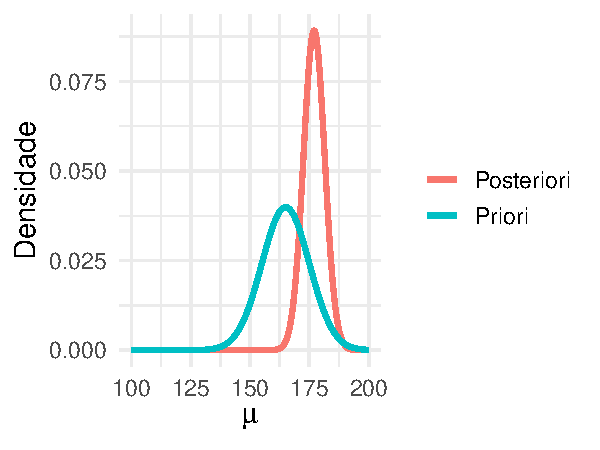
\includegraphics[width=\maxwidth]{./figures/normal_normal-1} 

}

\caption[Distribuições a priori e a posteriori (depois de observamos um indivíduo com 1,8m) para a altura média de um brasileiro]{Distribuições a priori e a posteriori (depois de observamos um indivíduo com 1,8m) para a altura média de um brasileiro}\label{fig:normal_normal}
\end{figure}

\end{knitrout}

\end{example}

A seguir, consideraremos o caso em que
$\mu$ é conhecido e $\tau^{2}$ é desconhecido.
\begin{lemma}
 Se $\mu$ é conhecido e
 $X|\tau^{2} \sim \text{N}(\mu,\tau^{2})$, então
 \begin{align*}
  \mathcal{P} = \left\{f: \mathbb{R} \rightarrow \mathbb{R}^{+}: f(\tau^{2}) = K \cdot \left(\tau^{2}\right)^{\alpha-1} \cdot \exp(-\beta \tau^{2}) \right\}
 \end{align*}
 é conjugada de $f(x|\tau^{2})$.
 Note que todas as densidades em $\mathcal{P}$ são
 da forma $\text{Gamma}(\alpha,\beta)$.
 Também, se $\tau^{2} \sim \text{Gamma}(\alpha,\beta)$,
 então
 \begin{align*}
  \tau^{2}|X \sim \text{Gamma}\left(\alpha+\frac{1}{2},
  \beta+\frac{(X-\mu)^{2}}{2}\right)
 \end{align*}
\end{lemma}

\begin{proof}
 \begin{align*}
  f(\tau^{2}) \cdot f(x|\mu)
  &= K \cdot \left(\tau^{2}\right)^{\alpha-1} \cdot \exp(-\beta \tau^{2}) \cdot \frac{\tau}{\sqrt{2\pi}} \cdot \exp\left(-\frac{\tau^{2}(x-\mu)^{2}}{2}\right)
  \nonumber \\
  &\propto \left(\tau^{2}\right)^{\alpha-1} \cdot \tau \cdot \exp(-\beta \tau^{2}) \cdot \exp\left(-\frac{\tau^{2}(x-\mu)^{2}}{2}\right) \\
  &= \left(\tau^{2}\right)^{\alpha+\frac{1}{2}-1} \cdot \exp\left(-\left(\beta+\frac{(x-\mu)^{2}}{2}\right)\tau^{2}\right) \in \mathcal{P}
 \end{align*}
 Também observe que $f(\tau^{2}) \cdot f(x|\tau^{2})$ é
 proporcional à densidade de uma Gamma com parâmetros
 $\alpha+\frac{1}{2}$ e
 $\left(\beta+\frac{(x-\mu)^{2}}{2}\right)$. Portanto,
 \begin{align*}
  \tau^{2}|X \sim \text{Gamma}\left(\alpha+\frac{1}{2},
  \beta+\frac{(x-\mu)^{2}}{2}\right).
 \end{align*}
\end{proof}

Finalmente, prosseguimos ao caso em que
tanto $\mu$ quanto $\tau^{2}$ são desconhecidos
\begin{lemma}
 \label{lemma:conjugate_normal_mean_precision}
 Se $X|\mu,\tau^{2} \sim \text{N}(\mu,\tau^{2})$,
 então
 \begin{align*}
  \mathcal{P} = \left\{f: \mathbb{R} \rightarrow \mathbb{R}^{+}: f(\mu) = K \cdot (\tau^{2})^{\alpha-1}\exp(-\beta \tau^{2})\exp\left(-\frac{\lambda\tau^{2}(\mu-\mu_{0})^{2}}{2}\right)\right\}
 \end{align*}
 é conjugada de $f(x|\mu,\tau^{2})$.
 As densidades em $\mathcal{P}$ pertencem à
 família bivariada Normal-Gamma com parâmetros
 $(\mu_{0},\lambda,\alpha,\beta)$. Note que se 
 $(\mu,\tau^{2})$ tem distribuição Normal-Gamma,
 então $\mu$ e $\tau^{2}$ não são independentes.
 De fato, se $(\mu,\tau^{2}) \sim \text{Normal-Gamma}(\mu_{0},\lambda,\alpha,\beta)$, então temos:
 \begin{align*}
  \tau^{2} \sim \text{Gamma}(\alpha, \beta) \\
  \mu|\tau^{2} \sim \text{Normal}(\mu_{0},\lambda \tau^{2})
 \end{align*}
 Também, se $(\mu,\tau^{2}) \sim \text{Normal-Gamma}(\alpha,\beta,\mu_{0},\lambda)$, então
 \begin{align*}
  (\mu,\tau^{2})|X \sim \text{Normal-Gamma}\left(\frac{(\lambda\mu_{0}+X)}{\lambda+1}, \lambda+1, \alpha+\frac{1}{2}, \beta + \frac{\lambda(\mu_{0}-X)^{2}}{2(\lambda+1)} \right)
 \end{align*}
\end{lemma}

\begin{proof}
 Note que, nos passos a seguir, tanto
 $\mu$ quanto $\tau^{2}$ são desconhecidos.
 Assim, expressões que dependam de
 quaisquer destes parâmetros não são constantes.
 \begin{align}
  \label{eqn:conjugate_normal_mean_variance_1}
  f(\mu,\tau^{2}|x)
  &\propto f(\mu,\tau^{2})f(x|\mu,\tau^{2})	\nonumber \\
  &= K \cdot (\tau^{2})^{\alpha-1}\exp(-\beta \tau^{2})\exp\left(-\frac{\lambda\tau^{2}(\mu-\mu_{0})^{2}}{2}\right) \cdot \frac{\tau}{\sqrt{2\pi}}\exp\left(-\frac{\tau^{2}(x-\mu)^{2}}{2}\right) \nonumber \\
  &\propto (\tau^{2})^{\alpha+\frac{1}{2}-1} \cdot \exp(-\beta \tau^{2}) \cdot \exp\left(-\frac{\lambda\tau^{2}(\mu^{2}-2\mu\mu_{0}+\mu_{0}^{2})}{2}\right) \cdot \exp\left(-\frac{\tau^{2}(x^{2}-2x\mu+\mu^{2})}{2}\right)	\nonumber \\
  &= (\tau^{2})^{\alpha+\frac{1}{2}-1} \cdot \exp\left(-\left(\beta + \frac{x^{2}}{2} + \frac{\lambda\mu_{0}^{2}}{2}\right)\tau^{2}\right) \cdot \exp\left(-\frac{\lambda\tau^{2}\mu^{2}-2\lambda\tau^{2}\mu\mu_{0}+\tau^{2}\mu^{2}-2\tau^{2}x\mu}{2}\right) \nonumber \\
  &= (\tau^{2})^{\alpha+\frac{1}{2}-1} \cdot \exp\left(-\left(\beta + \frac{x^{2}}{2} + \frac{\lambda\mu_{0}^{2}}{2}\right)\tau^{2}\right) \cdot \exp\left(-\frac{(\lambda+1)\tau^{2}\mu^{2}-2(\lambda\tau^{2}\mu_{0}+\tau^{2}x)\mu}{2}\right)
 \end{align}
 Similarmente ao caso em que $\tau^{2}$ é conhecido,
 desejamos completar o quadrado em função de
 $\mu$ para obter o formato da distribuição normal.
 Usamos novamente a \cref{eqn:conjugate_normal_2} para
 obter
 \begin{align*}
  \begin{cases}
   a^{2} &= (\lambda+1)\tau^{2} \\
   2ab &= 2(\lambda\tau^{2}\mu_{0}+\tau^{2}x)
  \end{cases}
 \end{align*}
 e obtemos
 \begin{align}
  \label{eqn:conjugate_normal_mean_variance_2}
  \begin{cases}
   a &= \sqrt{\lambda+1} \cdot \tau \\
   b &= \frac{\tau(\lambda\mu_{0}+x)}{\sqrt{\lambda+1}}
  \end{cases}
 \end{align}
 Substituindo a
 \cref{eqn:conjugate_normal_mean_variance_2}
 em \cref{eqn:conjugate_normal_mean_variance_1}, obtemos:
 \begin{align*}
  f(\mu,\tau^{2}|x) &\propto (\tau^{2})^{\alpha+\frac{1}{2}-1} \cdot \exp\left(-\left(\beta + \frac{x^{2}}{2} + \frac{\lambda\mu_{0}^{2}}{2}\right)\tau^{2}\right) \cdot \exp\left(-\frac{a^{2}\mu^{2}-2ab\mu}{2}\right) \\
  &= (\tau^{2})^{\alpha+\frac{1}{2}-1} \cdot \exp\left(-\left(\beta + \frac{x^{2}}{2} + \frac{\lambda\mu_{0}^{2}}{2}\right)\tau^{2}\right) \cdot \exp\left(-\frac{a^{2}\mu^{2}-2ab\mu+b^{2}}{2}\right) \cdot \exp\left(\frac{b^{2}}{2}\right) \\
  &= (\tau^{2})^{\alpha+\frac{1}{2}-1} \cdot \exp\left(-\left(\beta + \frac{x^{2}}{2} + \frac{\lambda\mu_{0}^{2}}{2}\right)\tau^{2} + \frac{b^{2}}{2}\right) \cdot \exp\left(-\frac{a^{2}\left(\mu-\frac{b}{a}\right)^{2}}{2}\right) \\
  &= (\tau^{2})^{\alpha+\frac{1}{2}-1} \cdot \exp\left(-\left(\beta + \frac{x^{2}}{2} + \frac{\lambda\mu_{0}^{2}}{2}\right)\tau^{2} + \frac{\tau^{2} (\lambda\mu_{0}+x)^{2}}{2(\lambda+1)}\right) \cdot \exp\left(-\frac{a^{2}\left(\mu-\frac{b}{a}\right)^{2}}{2}\right) \\
  &= (\tau^{2})^{\alpha+\frac{1}{2}-1} \cdot \exp\left(-\left(\beta + \frac{x^{2}}{2} + \frac{\lambda\mu_{0}^{2}}{2}\right)\tau^{2} + \frac{\tau^{2} (\lambda\mu_{0}+x)^{2}}{2(\lambda+1)}\right) \cdot \exp\left(-\frac{a^{2}\left(\mu-\frac{b}{a}\right)^{2}}{2}\right) \\
  &= (\tau^{2})^{\alpha+\frac{1}{2}-1} \cdot \exp\left(-\left(\beta + \frac{\lambda(\mu_{0}-x)^{2}}{2(\lambda+1)}\right)\tau^{2}\right) \cdot \exp\left(-\frac{a^{2}\left(\mu-\frac{b}{a}\right)^{2}}{2}\right)	\\
  &= (\tau^{2})^{\alpha+\frac{1}{2}-1} \cdot \exp\left(-\left(\beta + \frac{\lambda(\mu_{0}-x)^{2}}{2(\lambda+1)}\right)\tau^{2}\right) \cdot \exp\left(-\frac{(\lambda+1)\tau^{2}\left(\mu-\frac{(\lambda\mu_{0}+x)}{\lambda+1}\right)^{2}}{2}\right) \in \mathcal{P}
 \end{align*}
 Do resultado acima, podemos concluir que
 \begin{align*}
  (\mu,\tau^{2})|X \sim \text{Normal-Gamma}\left(\frac{(\lambda\mu_{0}+X)}{\lambda+1}, \lambda+1, \alpha+\frac{1}{2}, \beta + \frac{\lambda(\mu_{0}-X)^{2}}{2(\lambda+1)} \right)
 \end{align*}
\end{proof}


\begin{example}
 Considere novamente o Exemplo
 \ref{ex:altura}, mas vamos agora assumir 
 que a altura de um brasileiro selecionado ao acaso, 
 $X$, é tal que
 $X|\mu \sim N(\mu,\tau^2)$, 
 com $\tau^2$ desconhecido.
 Agora precisamos fazer a inferência simultaneamente 
 para $\mu$ e $\tau^2$
 Para tanto, vamos assumir que
 $(\mu,\tau^2) \sim \mbox{Normal-Gamma}(1.65,1,6,0.05)$.
 Como $x=1.8$,
 $(\mu,\tau^2)|x \sim 
 \mbox{Normal-Gamma}(1.725, 2, 6.5, 0.055625)$. 
 A Figura \ref{fig:normal_gamma} mostra 
 a distribuição a priori e 
 a distribuição a posteriori 
 para essa observação. 

\begin{knitrout}
\definecolor{shadecolor}{rgb}{0.969, 0.969, 0.969}\color{fgcolor}\begin{kframe}
\begin{alltt}
\hlkwd{library}\hlstd{(ggplot2)}
\hlkwd{library}\hlstd{(patchwork)}

\hlkwd{set.seed}\hlstd{(}\hlnum{0}\hlstd{)}
\hlstd{sigma} \hlkwb{<-} \hlnum{0.075}
\hlstd{mu} \hlkwb{<-} \hlnum{1.70}
\hlcom{# X ~ N(mu, sigma)}
\hlstd{altura} \hlkwb{<-} \hlnum{1.80}

\hlstd{atualiza} \hlkwb{<-} \hlkwa{function}\hlstd{(}\hlkwc{hparam}\hlstd{,} \hlkwc{x}\hlstd{)}
\hlstd{\{}
  \hlkwd{list}\hlstd{(}
    \hlkwc{mu0} \hlstd{= (hparam}\hlopt{$}\hlstd{lambda}\hlopt{*}\hlstd{hparam}\hlopt{$}\hlstd{mu0}\hlopt{+}\hlstd{x)}\hlopt{/}\hlstd{(hparam}\hlopt{$}\hlstd{lambda}\hlopt{+}\hlnum{1}\hlstd{),}
    \hlkwc{lambda} \hlstd{= hparam}\hlopt{$}\hlstd{lambda} \hlopt{+} \hlnum{1}\hlstd{,}
    \hlkwc{alpha} \hlstd{= hparam}\hlopt{$}\hlstd{alpha} \hlopt{+} \hlnum{.5}\hlstd{,}
    \hlkwc{beta} \hlstd{= hparam}\hlopt{$}\hlstd{beta} \hlopt{+}
      \hlstd{(hparam}\hlopt{$}\hlstd{lambda}\hlopt{*}\hlstd{(hparam}\hlopt{$}\hlstd{mu0}\hlopt{-}\hlstd{x)}\hlopt{^}\hlnum{2}\hlstd{)}\hlopt{/}\hlstd{(}\hlnum{2}\hlopt{*}\hlstd{(hparam}\hlopt{$}\hlstd{lambda}\hlopt{+}\hlnum{1}\hlstd{))}
  \hlstd{)}
\hlstd{\}}

\hlstd{hparam_prior} \hlkwb{<-} \hlkwd{list}\hlstd{(}
  \hlkwc{mu0} \hlstd{=} \hlnum{1.65}\hlstd{,}
  \hlkwc{lambda} \hlstd{=} \hlnum{1}\hlstd{,}
  \hlkwc{beta} \hlstd{=} \hlnum{0.05}\hlstd{,}
  \hlkwc{alpha} \hlstd{=} \hlnum{120}\hlopt{*}\hlnum{0.05}
\hlstd{)}

\hlstd{grid_bivariado} \hlkwb{<-} \hlkwd{expand.grid}\hlstd{(}
  \hlkwc{mu} \hlstd{=} \hlkwd{seq}\hlstd{(}\hlnum{1.4}\hlstd{,} \hlnum{1.8}\hlstd{,} \hlkwc{length.out} \hlstd{=} \hlnum{300}\hlstd{),}
  \hlkwc{tau2} \hlstd{=} \hlkwd{seq}\hlstd{(}\hlnum{60}\hlstd{,} \hlnum{200}\hlstd{,} \hlkwc{length.out} \hlstd{=} \hlnum{300}\hlstd{)}
\hlstd{)}

\hlcom{# retorna f(grid_bivariado|hparam)}
\hlstd{densidade} \hlkwb{<-} \hlkwa{function}\hlstd{(}\hlkwc{grid_bivariado}\hlstd{,} \hlkwc{hparam}\hlstd{)}
\hlstd{\{}
  \hlkwd{dgamma}\hlstd{(grid_bivariado}\hlopt{$}\hlstd{tau2,}
         \hlstd{hparam}\hlopt{$}\hlstd{alpha,}
         \hlstd{hparam}\hlopt{$}\hlstd{beta)}\hlopt{*}
    \hlkwd{dnorm}\hlstd{(grid_bivariado}\hlopt{$}\hlstd{mu,}
          \hlstd{hparam}\hlopt{$}\hlstd{mu0,}
          \hlkwd{sqrt}\hlstd{(}\hlnum{1}\hlopt{/}\hlstd{(hparam}\hlopt{$}\hlstd{lambda}\hlopt{*}\hlstd{grid_bivariado}\hlopt{$}\hlstd{tau2)))}
\hlstd{\}}

\hlstd{plot_densidade} \hlkwb{<-} \hlkwa{function}\hlstd{(}\hlkwc{grid_bivariado}\hlstd{,} \hlkwc{hparam}\hlstd{)}
\hlstd{\{}
  \hlstd{dados_plot} \hlkwb{<-} \hlkwd{data.frame}\hlstd{(}
    \hlkwc{mu} \hlstd{= grid_bivariado}\hlopt{$}\hlstd{mu,}
    \hlkwc{tau2} \hlstd{= grid_bivariado}\hlopt{$}\hlstd{tau2,}
    \hlkwc{densidade} \hlstd{=} \hlkwd{densidade}\hlstd{(grid_bivariado, hparam)}
  \hlstd{)}

  \hlkwd{ggplot}\hlstd{(dados_plot,}
         \hlkwd{aes}\hlstd{(mu, tau2,} \hlkwc{fill} \hlstd{= densidade))} \hlopt{+}
    \hlkwd{geom_raster}\hlstd{(}\hlkwc{interpolate} \hlstd{=} \hlnum{TRUE}\hlstd{)} \hlopt{+}
    \hlkwd{ggtitle}\hlstd{(}\hlkwd{paste0}\hlstd{(}\hlstr{"Prior"}\hlstd{))} \hlopt{+}
    \hlkwd{coord_cartesian}\hlstd{(}\hlkwc{xlim}\hlstd{=}\hlkwd{range}\hlstd{(grid_bivariado}\hlopt{$}\hlstd{mu),}
                    \hlkwc{ylim}\hlstd{=}\hlkwd{range}\hlstd{(grid_bivariado}\hlopt{$}\hlstd{tau2))} \hlopt{+}
    \hlkwd{scale_fill_gradientn}\hlstd{(}\hlkwc{colours} \hlstd{=} \hlkwd{terrain.colors}\hlstd{(}\hlnum{100}\hlstd{))} \hlopt{+}
    \hlkwd{theme_bw}\hlstd{()} \hlopt{+}
    \hlkwd{theme}\hlstd{(}\hlkwc{axis.text}\hlstd{=}\hlkwd{element_text}\hlstd{(}\hlkwc{size}\hlstd{=}\hlnum{18}\hlstd{),}
          \hlkwc{axis.title}\hlstd{=}\hlkwd{element_text}\hlstd{(}\hlkwc{size}\hlstd{=}\hlnum{20}\hlstd{,}\hlkwc{face}\hlstd{=}\hlstr{"bold"}\hlstd{))} \hlopt{+}
    \hlkwd{xlab}\hlstd{(}\hlkwd{expression}\hlstd{(mu))} \hlopt{+}
    \hlkwd{ylab}\hlstd{(}\hlkwd{expression}\hlstd{(tau}\hlopt{^}\hlnum{2}\hlstd{))}
\hlstd{\}}

\hlstd{aux1} \hlkwb{=} \hlkwd{plot_densidade}\hlstd{(grid_bivariado, hparam_prior)}
\hlstd{aux2} \hlkwb{=} \hlkwd{plot_densidade}\hlstd{(grid_bivariado,}
                      \hlkwd{atualiza}\hlstd{(hparam_prior, altura))}

\hlstd{aux1}
\end{alltt}
\end{kframe}\begin{figure}[t]

{\centering 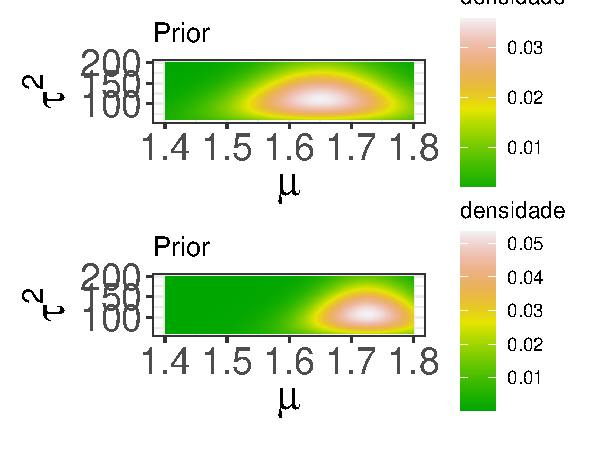
\includegraphics[width=\maxwidth]{figure/normal_gamma-1} 

}

\caption[Distribuições a priori e a posteriori (depois de observamos um indivíduo com 1,8m) para a altura média de um brasileiro]{Distribuições a priori e a posteriori (depois de observamos um indivíduo com 1,8m) para a altura média de um brasileiro}\label{fig:normal_gamma-1}
\end{figure}

\begin{kframe}\begin{alltt}
\hlstd{aux2}
\end{alltt}
\end{kframe}\begin{figure}[t]

{\centering 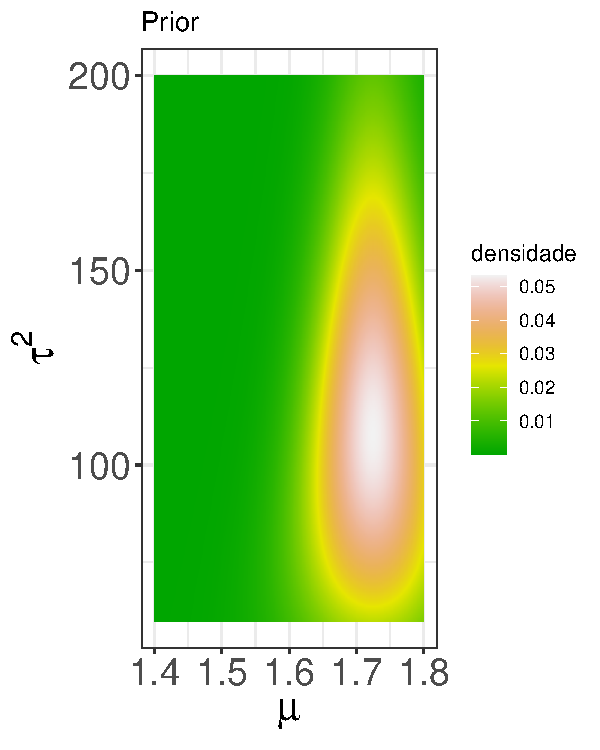
\includegraphics[width=\maxwidth]{figure/normal_gamma-2} 

}

\caption[Distribuições a priori e a posteriori (depois de observamos um indivíduo com 1,8m) para a altura média de um brasileiro]{Distribuições a priori e a posteriori (depois de observamos um indivíduo com 1,8m) para a altura média de um brasileiro}\label{fig:normal_gamma-2}
\end{figure}

\end{knitrout}
\end{example}

\subsubsection*{Exercícios}

\begin{exercise}
 \label{ex:conjugate-normal-normal}
 Considere que, dado $\mu$,
 $X_{1},\ldots,X_{n}$ são i.i.d. e
 $X_{i} \sim N(\mu,\tau^{2})$, com
 $\tau^{2}$ conhecido. Se
 $\mu \sim N(\mu_{0},\tau_{0}^{2})$, então:
 \begin{enumerate}[label=(\alph*)]
  \item Ache a posteriori para
  $\mu|X_{1},\ldots,X_{n}$.
  \item Determine 
  $\lim_{n \rightarrow \infty}\E[\mu|X_{1},\ldots,X_{n}]$.
  \item Determine
  $\lim_{n \rightarrow \infty}\V[\mu|X_{1},\ldots,X_{n}]$.
  \item Interprete em suas próprias palavras os
  resultados obtidos nos itens anteriores.
 \end{enumerate}
\end{exercise}

\solution{\textbf{Solução}:
 \begin{enumerate}[label=(\alph*)]
  \item
  \begin{align*}
   f(\mu) \cdot f(x_{1},\ldots,x_{n}|\mu)
   &= f(\mu)\prod_{i=1}^{n}{f(x_{i}|\mu)} \\
   &\propto \exp\left(-\frac{\tau_{0}^{2}(\mu-\mu_{0})^{2}}{2}\right) \cdot \prod_{i=1}^{n}{\exp\left(-\frac{\tau^{2}(x_{i}-\mu)^{2}}{2}\right)} \\
   &= \exp\left(-\frac{\tau_{0}^{2}\mu^{2}-2\tau_{0}^{2}\mu\mu_{0}+\tau_{0}^{2}\mu_{0}^{2}}{2}\right) \cdot \exp\left(-\frac{n\tau^{2}\mu^{2}-2\tau^{2}\mu \sum_{i=1}^{n}{x_{i}}+ \tau^{2}\sum_{i=1}^{n}{x_{i}^{2}}}{2}\right)	\nonumber \\
   &\propto \exp\left(-\frac{\tau_{0}^{2}\mu^{2}-2\tau_{0}^{2}\mu\mu_{0}+n\tau^{2}\mu^{2}-2n\tau^{2}\mu \bar{x}}{2}\right) \\
   &= \exp\left(-\frac{(\tau_{0}^{2}+n\tau^{2})\mu^{2}-2(\tau_{0}^{2}\mu_{0}+n\tau^{2}\bar{x})\mu}{2}\right)
  \end{align*}
  Realizando uma substituição de acordo com a
  \cref{eqn:conjugate_normal_2}, obtemos
  \begin{align*}
   \begin{cases}
    a^{2} &= \tau_{0}^{2}+n\tau^{2} \\
    2ab &= 2(\tau_{0}^{2}\mu_{0}+n\tau^{2}\bar{x})
   \end{cases}
  \end{align*}
  e
  \begin{align}
   \begin{cases}
    a &= \sqrt{\tau_{0}^{2}+n\tau^{2}} \\
    b &= \frac{\tau_{0}^{2}\mu_{0}+n\tau^{2}\bar{x}}
    {\sqrt{\tau_{0}^{2}+n\tau^{2}}}
   \end{cases}
  \end{align}
  Realizando esta substituição na
  \cref{eqn:conjugate_normal_1}, obtemos:
  \begin{align*}
   f(\mu) \cdot f(x|\mu)
   &\propto \exp\left(-\frac{a^{2}\mu^{2}
   -2ab\mu}{2}\right) \\
   &\propto \exp\left(-\frac{a^{2}\mu^{2}
   -2ab\mu+b^{2}}{2}\right)
   & \exp(b^{2}/2) \text{ é constante} \\
   &= \exp\left(-\frac{(a\mu-b)^{2}}{2}\right)
   & \cref{eqn:conjugate_normal_2} \\
   &= \exp\left(-\frac{a^{2}\left(\mu
   -\frac{b}{a}\right)^{2}}{2}\right) \in \mathcal{P}
  \end{align*}
  Também observe que $f(\mu) \cdot f(x|\mu)$ é
  proporcional à densidade de uma normal com
  $\mu=\frac{b}{a}$ e $\tau^{2}=a^{2}$.
  Substituindo os valores obtidos na   
  \cref{eqn:conjugate_normal_3} temos que
  \begin{align*}
   \mu|X_{1},\ldots,X_{n} \sim
   N\left(\frac{\tau_{0}^{2}\mu_{0}+n\tau^{2}\bar{x}}{\tau_{0}^{2}+n\tau^{2}},\tau_{0}^{2}+n\tau^{2}\right)
  \end{align*}

  \item
  \begin{align*}
   \lim_{n \rightarrow \infty}E[\mu|X_{1},\ldots,X_{n}]	
   &= \lim_{n \rightarrow \infty}
   \frac{\tau_{0}^{2}\mu_{0}+n\tau^{2}\bar{X}}
   {\tau_{0}^{2}+n\tau^{2}} \\
   &= \lim_{n \rightarrow \infty}
   \frac{\tau_{0}^{2}\mu_{0}/n +\tau^{2}\bar{X}}
   {\tau_{0}^{2}/n +\tau^{2}} = \bar{X} \\
  \end{align*}

  \item 
  \begin{align*}
   \lim_{n \rightarrow \infty}
   \V[\mu|X_{1},\ldots,X_{n}]
   &= \lim_{n \rightarrow \infty}
   \frac{1}{\tau_{0}^{2}+n\tau^{2}} = 0
  \end{align*}
 \end{enumerate}
}{}

\begin{exercise}
 Considere que, dado $\tau^{2}$,
 $X_{1},\ldots,X_{n}$ são i.i.d. e
 $X_{i} \sim N(\mu,\tau^{2})$, com
 $\mu$ conhecido. Considere que
 $\tau^{2} \sim \text{Gamma}(\alpha,\beta)$.
 \begin{enumerate}[label=(\alph*)]
  \item Ache a posteriori para
  $\tau^{2}|X_{1},\ldots,X_{n}$.
  \item Derive $\lim_{n \rightarrow \infty}\E[\tau^{2}|X_{1},\ldots,X_{n}]$.
  \item Interprete em suas próprias palavras os
  resultados obtidos nos itens anteriores.
 \end{enumerate}
\end{exercise}

\solution{\textbf{Solução}:
 \begin{enumerate}[label=(\alph*)]
  \item
  \begin{align*}
   f(\tau^{2}|x_{1},\ldots,x_{n})
   &\propto f(\tau^{2})
   f(x_{1},\ldots,x_{n}|\tau^{2}) \\
   &= f(\tau^{2})\prod_{i=1}^{n}{f(x_{i}|\tau^{2})}	\\
   &\propto \left(\tau^{2}\right)^{\alpha-1} \cdot \exp\left(-\beta \tau^{2}\right) \cdot \tau^{n} \cdot \prod_{i=1}^{n}{\exp\left(-\frac{\tau^{2}(x_{i}-\mu)^{2}}{2}\right)} \\
   &= \left(\tau^{2}\right)^{\alpha+\frac{n}{2}-1} \cdot \exp\left(-\left(\beta+ \frac{\sum_{i=1}^{n}{(x_{i}-\mu)^{2}}}{2}\right)\tau^{2}\right)
  \end{align*}
  Portanto,
  \begin{align*}
   \tau^{2}|X_{1},\ldots,X_{n} \sim
   \text{Gamma}\left(\alpha+\frac{n}{2},
   \beta+\frac{\sum_{i=1}^{n}{(x_{i}-\mu)^{2}}}{2}\right)
  \end{align*}
  \item
  \begin{align*} 
   \limn\E[\tau^{2}|X_{1},\ldots,X_{n}]
   &= \lim_{n \rightarrow \infty}
   \frac{\alpha+\frac{n}{2}}
   {\beta+ \frac{\sum_{i=1}^{n}{(X_{i}-\mu)^{2}}}{2}} \\
   &= \limn\frac{n}{\sum_{i=1}^{n}{(X_{i}-\mu)^{2}}}
   = \tau^2
  \end{align*}
 \end{enumerate}
}{}

\subsubsection{A família exponencial}

A família exponencial é uma generalização de 
diversas famílias de distribuições.

\begin{definition}
 \label{defn:exponential-family}
 Dizemos que, dado um vetor de parâmetros $\theta$,
 um vetor de dados, $X$, 
 tem distribuição pertencente à família exponencial se o suporte de $x$ não
 depende de $\theta$ e se
 \begin{align*}
  f(x|\theta) 
  &= h(x) \exp\left(g(\theta) \cdot T(x)
  - A(\theta)\right)
 \end{align*}
 onde $g(\theta)$ e $T(x)$ são
 funções multivariadas dos parâmetros e dos dados.
\end{definition}

Note que, para cada valor de $\theta$,
$A(\theta)$ é o valor que faz com que
$f(x|\theta)$ integre $1$.
Assim, $A(\theta)$ é completamente especificado
em função dos demais elementos da família exponencial.

\begin{example}
 \label{example:exponential_family_binomial}
 Considere que $X|\theta \sim \text{Binomial}(n,\theta)$.
 \begin{align*}
  f(x|\theta)
  &= {n \choose x}\theta^{x}(1-\theta)^{n-x} \\
  &= {n \choose x}\exp\left(x\log(\theta)
  +(n-x)\log(1-\theta)\right) \\
  &= {n \choose x}\exp\left(x \cdot \log\left(\frac{\theta}{1-\theta}\right) +n\log(1-\theta)\right)
 \end{align*}
 Portanto, $f(x|\theta)$ pertence à
 família exponencial, tomando-se 
 \begin{align*}
  \begin{cases}
   h(x) &= {n \choose x} \\
   T(X) &= x \\
   g(\theta) 
   &= \log\left(\frac{\theta}{1-\theta}\right) \\
   A(\theta) &= -n\log(1-\theta)
  \end{cases}
 \end{align*}
\end{example}

\begin{example}
 Considere que $\theta=(\mu,\tau^{2})$ e
 $X|\theta \sim \text{Normal}(\mu,\tau^{2})$.
 \begin{align*}
  f(x|\mu,\tau^{2})
  &= \frac{\tau}{\sqrt{2\pi}}\exp\left(-\frac{\tau^{2}(x-\mu)^{2}}{2}\right) \\
  &= \frac{1}{\sqrt{2\pi}}\exp\left(-\frac{\tau^{2}x^{2}-2\tau^{2}x\mu +\tau^{2}\mu^{2}}{2} +\log(\tau)\right) \\
  &= \frac{1}{\sqrt{2\pi}}\exp\left((x,-x^{2}/2) \cdot (\tau^{2}\mu, \tau^{2}) -\left(\frac{\tau^{2}\mu^{2}}{2}-\log(\tau)\right)\right)
 \end{align*}
 Portanto, $f(x|\theta)$ pertence à
 família exponencial, tomando-se 
 \begin{align*}
  \begin{cases}
   h(x) &= \frac{1}{\sqrt{2\pi}} \\
   T(X) &= (x,-x^{2}/2) \\
   g(\theta) &= (\tau^{2}\mu, \tau^{2}) \\
   A(\theta) &= \left(\frac{\tau^{2}\mu^{2}}{2}
   -\log(\tau)\right)
  \end{cases}
 \end{align*}
\end{example}

Muitas outras distribuições pertencem à
família exponencial. Por exemplo, a Binomial-Negativa,
a Poisson, a Multinomial, a Hipergeométrica,
a Geométrica, a log-Normal, a Exponencial,
a Gamma, a Gamma-Inversa, a Beta, a Weibull e a Laplace.

Além de incluir diversas distribuições,
a família exponencial também apresenta
propriedades importantes. No contexto desta seção, 
podemos derivar a família conjugada para
um membro da família exponencial.

\begin{lemma}
 \label{lemma:exponential-family-conjugate}
 Se $f(x|\theta)$ faz parte da família exponencial,
 isto é, $f(x|\theta) = h(x) \exp\left(g(\theta) \cdot T(x) - A(\theta)\right)$, então
 \begin{align*}
  \mathcal{P} = \left\{f(\theta): f(\theta) 
  = K \cdot \exp\left(-\alpha A(\theta) + g(\theta) \cdot \beta\right) \right\}
 \end{align*}
 é conjugada a $f(x|\theta)$.
\end{lemma}

\begin{proof}
 Note que
 \begin{align*}
  f(\theta)f(x|\mu)
  &\propto \exp\left(-\alpha A(\theta)
  +g(\theta) \cdot \beta\right) \cdot h(x)
  \cdot \exp\left(g(\theta) \cdot T(x)
  -A(\theta)\right) \\
  &\propto \exp\left(-(\alpha+1)A(\theta)
  +g(\theta) \cdot (\beta+T(x))\right) \in \mathcal{P}
 \end{align*}
 Portanto, $\mathcal{P}$ é conjugada de $f(x|\theta)$.
 Similarmente, para o caso em que
 $X_{1},\ldots,X_{n}$ são i.i.d. dado $\theta$,
 obtemos
 \begin{align*}
  f(\theta)f(x_{1},\ldots,x_{n}|\mu)
  &=f(\theta)\prod_{i=1}^{n}{f(x_{i}|\theta)} \\
  &\propto \exp\left(-\alpha A(\theta)
  +g(\theta) \cdot \beta\right) \cdot \prod_{i=1}^{n}
  {\exp\left(g(\theta) \cdot T(x_{i})
  -A(\theta)\right)} \\
  &\propto \exp\left(-(\alpha+n)A(\theta)
  +g(\theta) \cdot \left(\beta+\sum_{i=1}^{n}
  {T(x_{i})}\right)\right) \in \mathcal{P}
 \end{align*}
\end{proof}

\begin{example}
 \label{example:exponential-family-binomial}
 Considere que
 $X|\theta \sim \text{Binomial}(n,\theta)$.
 Vimos no \cref{example:exponential_family_binomial}
 que $f(x|\theta)$ pertence à família exponencial.
 Portanto, temos que
 \begin{align*}
  \mathcal{P} = \{f(\theta) =K
  \cdot \exp\left(-\alpha A(\theta)
  +g(\theta) \cdot \beta \right) \}
 \end{align*}
 é conjugada de $f(x|\theta)$.
 Substituindo os termos encontrados no
 \cref{example:exponential_family_binomial}, obtemos
 \begin{align*}
  \mathcal{P} &= \left\{f(\theta) = K \cdot \exp\left(\alpha n\log(1-\theta) +\log\left(\frac{\theta}{1-\theta}\right) \cdot \beta \right) \right\} \\
  &= \{f(\theta) = K(1-\theta)^{n\alpha-\beta} \theta^{\beta} \}
 \end{align*}
 Assim encontramos que a família Beta é
 conjugada da Binomial, assim como na
 \cref{sec:conjugate_beta_binomial}.
 Observe que, para que seja possível obter
 $\int{f(\theta)d\theta}=1$, é necessário que
 $n\alpha > \beta$ e $\beta > 0$. 
\end{example}

Ao aplicar o \cref{lemma:exponential-family-conjugate},
nem sempre é imediato quais valores de
$\alpha$ e $\beta$ são tais que
$f(\theta)$ é integrável.
No \cref{example:exponential-family-binomial}
verificamos que, para obter esta condição, era
necessário que $n\alpha > \beta$ e $\beta > 0$.
Esta análise é generalizada por um teorema em \citet{Diaconis1979} que é descrito a seguir.

\begin{theorem}
 \label{theorem:exponencial-propriety}
 Considere que $X \in \chi$,
 $\theta \in \mathbb{R}^{d}$ e
 $f(x|\theta)$ está na forma canônica da
 família exponencial, isto é,
 $f(x|\theta) = h(x) \exp\left(\theta \cdot T(x) - A(\theta)\right)$.
 A função $f(\theta) = \exp\left(-\alpha A(\theta) +\theta \cdot \beta \right)$
 é integrável se e somente se $\alpha > 0$ e
 $\frac{\beta}{\alpha} \in \text{Interior}[\text{Conv}[T[\chi]]]$.
\end{theorem}

\begin{example}
 Considere que
 $X|\theta \sim \text{Poisson}(\theta)$. Obtemos,
 \begin{align*}
  f(x|\theta)
  &= \frac{\exp(-\theta)\theta^{x}}{x!} \\
  &= (x!)^{-1} \exp(\log(\theta) \cdot x - \theta) \\
 \end{align*}
 Assim, definindo $\eta = \log(\theta)$, obtemos:
 \begin{align*}
  f(x|\eta)
  &= (x!)^{-1} \exp(\eta \cdot x - \exp(\eta))
 \end{align*}
 Conclua que $f(x|\eta)$ está na
 forma canônica da familia exponencial, tomando
 \begin{align*} 
  \begin{cases}
   h(x) &= (x!)^{-1} \\
   T(x) &= x \\
   A(\eta) &= \exp(\eta) \\
  \end{cases}
 \end{align*}
 Portanto, decorre do
 \cref{lemma:exponential-family-conjugate} que
 a seguinte familia é conjugada para $f(x|\eta)$
 \begin{align*}
  \mathcal{P} = \left\{f(\eta): f(\eta) \propto \exp(-\alpha\exp(\eta) + \eta \cdot \beta) \right\}
 \end{align*}
 Ademais, podemos aplicar o
 \cref{theorem:exponencial-propriety} para
 obter os valores de $\alpha$ e $\beta$ tais que
 $\exp(-\alpha\exp(\eta) + \eta \cdot \beta)$ é
 integrável. Obtemos que $\exp(-\alpha\exp(\eta) + \eta \cdot \beta)$ é integrável se e somente se
 $\alpha > 0$ e $\frac{\beta}{\alpha} \in \text{Interior}[\text{Conv}[T[\chi]]]$.
 Como $X|\theta \sim \text{Poisson}(\theta)$, obtemos
 $\chi = \mathbb{N}$.
 Assim, como $T(x) = x$, $T[\mathbb{N}] = \mathbb{N}$.
 Ademais, $\text{Conv}[\mathbb{N}] = \mathbb{R}^{+}$.
 Finalmente, $\text{Interior}[\mathbb{R}^+] = \mathbb{R}^{+}_{*}$.
 Portanto, $\text{Interior}[\text{Conv}[T[\chi]]] = \mathbb{R}^{+}_{*}$.
 Note que, se $\alpha > 0$, então
 $\frac{\beta}{\alpha} \in \mathbb{R}^{+}_{*}$
 se e somente se $\beta > 0$.
 Portanto, conclua do \cref{theorem:exponencial-propriety} que 
 $\exp(-\alpha\exp(\eta) + \eta \cdot \beta)$ é
 integrável se e somente $\alpha > 0$ e $\beta > 0$.
 Tomando a transformação $\log(\theta) = \eta$,
 obtemos que 
 $\big|\frac{d\log(\theta)}{d\theta}\big| \exp(-\alpha\theta + \log(\theta) \cdot \beta)$ é
 integrável se e somente se
 $\alpha > 0$ e $\beta > 0$. Assim,
 \begin{align*} 
  \mathcal{P}^{*} &= \left\{f(\theta):
  f(\theta) \propto \theta^{\beta-1}\exp(-\alpha \theta), \alpha > 0, \beta > 0\right\}
 \end{align*}
 é uma familia de distribuições integráveis.
 Ademais, decorre do
 \cref{lemma:exponential-family-conjugate} que
 $\mathcal{P}$ é conjugada para $f(x|\theta)$.
 Note que as densidades em $\mathcal{P}^{*}$
 correspondem à família de distribuições Gamma.
\end{example}

\subsubsection*{Exercícios}

\begin{exercise}
 O jogador $A$ acredita que a frequência com que 
 ela vence jogos de xadrez contra o jogador $B$
 segue uma distribuição $\text{Beta}(2,2)$.
 Em um torneio, o jogador $A$ joga quatro partidas contra
 o jogador $B$ até ganhar seu primeiro jogo.
 \begin{enumerate}[label=(\alph*)]
  \item Descreva os elementos do modelo estatístico Bayesiano.
  \item Antes de jogar contra $B$, em média quantas vezes
  o jogador $A$ acreditava que ele precisaria jogar
  até vencer contra o jogador $B$?
  \item Encontre a distribuição a posteriori para
 a frequência com que o jogador $A$ vence
 jogos contra o jogador $B$ após o torneio.
 \item Após o torneio, em média quantas partidas a mais
 o jogador $A$ acredita que precisaria jogar contra $B$
 para obter uma nova vitória?
 \end{enumerate}
\end{exercise}

\begin{exercise}
 Escolha duas de suas famílias de
 distribuições favoritas e descubra se
 elas pertencem ou não à família exponencial.
\end{exercise}

\begin{exercise}
 Se $X|\theta \sim \text{Geom}(\theta)$:
 \begin{enumerate}[label=(\alph*)]
  \item Mostre que $f(x|\theta)$ pertence à
  família exponencial.
  \item Ache a família conjugada para $f(x|\theta)$.
  \item Ache a posteriori para $\theta$ quando
  a priori é conjugada.
 \end{enumerate} 
\end{exercise}

\solution{\textbf{Solução}:
 \begin{enumerate}[label=(\alph*)]
  \item
  \begin{align*}
   f(x|\theta) &= \theta (1-\theta)^{x} \\
   &= \exp(\log(\theta) + \log(1-\theta)x) \\
   &= 1 \cdot \exp(\log(1-\theta) \cdot x
   +\log(\theta))
  \end{align*}
  Portanto, $f(x|\theta)$ pertence à
  família exponencial com:
  \begin{align*}
   \begin{cases}
    h(x) &= 1 \\
    g(\theta) &= \log(1-\theta) \\
    T(x) &= x \\
    A(\theta) &= -\log(\theta)
   \end{cases}
  \end{align*}
  
  \item
  \begin{align*}
   \mathcal{P}	&= \{f(\theta)
   =K \cdot (\exp(-A(\theta)))^{\alpha} \cdot \exp(g(\theta) \cdot \beta) \} \\
   &= \{f(\theta) 
   =K \cdot (\exp(\log(\theta)))^{\alpha} \cdot \exp(\log(1-\theta)\beta) \} \\
   &= \{f(\theta) =K \cdot \theta^{\alpha}
   (1-\theta)^{\beta}\}
  \end{align*}
  Portanto, a família Beta é conjugada a $f(x|\theta)$.
  \item
  \begin{align*}
   f(\theta|x)	&\propto f(\theta)f(x|\theta) \\
   &\propto \theta^{\alpha}(1-\theta)^{\beta}\theta (1-\theta)^{x} \\
   &= \theta^{\alpha+1}(1-\theta)^{\beta+x} \sim \text{Beta}(\alpha+2, \beta+x+1)
  \end{align*}
 \end{enumerate}
}{}

\begin{exercise}
 Se $X|\theta \sim \text{Exponencial}(\theta)$:
 \begin{enumerate}[label=(\alph*)]
  \item Mostre que $f(x|\theta)$ pertence à
  família exponencial.
  \item Ache a família conjugada para $f(x|\theta)$.
  \item Ache a posteriori para $\theta$ quando
  a priori é conjugada.
 \end{enumerate} 
\end{exercise}

\solution{\textbf{Solução}:
 \begin{enumerate}[label=(\alph*)]
  \item 
  \begin{align*}
   f(x|\theta)
   &= \theta \exp(-\theta x) \\
   &= 1 \cdot \exp(-\theta \cdot x +\log(\theta))
  \end{align*}
  Portanto, $f(x|\theta)$ pertence à
  família exponencial com:
  \begin{align*}
   \begin{cases}
    h(x) &= 1 \\
    g(\theta) &= -\theta \\
    T(x) &= x \\
    A(\theta) &= -\log(\theta)
   \end{cases}
  \end{align*}
  \item 
  \begin{align*}
   \mathcal{P}	&= \{f(\theta)
   =K \cdot (\exp(-A(\theta)))^{\alpha} \cdot \exp(g(\theta) \cdot \beta) \} \\
   &= \{f(\theta) 
   =K \cdot (\exp(\log(\theta)))^{\alpha} \cdot \exp(-\theta\beta) \} \\
   &= \{f(\theta) =K \cdot \theta^{\alpha}
   exp(-\theta \beta) \}
  \end{align*}
  Portanto, a família Gamma é conjugada a $f(x|\theta)$.
  \item 
  \begin{align*}
   f(\theta|x) &\propto f(\theta)f(x|\theta) \\
   &\propto \theta^{\alpha}\exp(-\theta \beta)
   \theta \exp(-\theta x) \\
   &= \theta^{\alpha+1}\exp(-\theta (\beta+x)
   \sim \text{Gamma}(\alpha+2, \beta+x)
  \end{align*}
 \end{enumerate}
}{}

\begin{exercise}
 Em uma população, a proporção de indivíduos com
 uma determinada doença é $\theta$.
 Considere que uma amostra de $100$ indivíduos é
 tomada da população. Para cada indivíduo, $i$,
 defina $Z_{i}$ como sendo a indicadora de que
 o indivíduo tem a doença.
 Um teste é realizado em cada um
 dos indivíduos da amostra.
 Este teste é tal que, se o indivíduo for doente,
 o teste acusa afirmativo certamente.
 Contudo, se o indivíduo não for doente,
 há uma probabilidade $0.1$ de um falso positivo.
 Para cada indivíduo, $i$, defina
 $X_{i}$ como sendo a indicadora de que
 o resultado do exame para o indivíduo $i$ foi positivo.
 Observou-se que $30$ indivíduos obtiveram
 o resultado positivo no teste.
 Note que as variáveis $Z_{i}$ não foram observadas.
 \begin{enumerate}[label=(\alph*)]
  \item Note que $X_{1}|\theta$ é uma Bernoulli.
  Use a lei da probabilidade total para mostrar que
  \begin{align*}
   X_{1}|\theta \sim \text{Bernoulli}(0.1 + 0.9\theta)
  \end{align*}
  \item Ache a distribuição de
  $\sum_{i=1}^{100}{X_{i}}|\theta$ e
  prove que ela pertence à família exponencial.
  \item Ache a família conjugada para
  $\sum_{i=1}^{100}{X_{i}}|\theta$.
  \item Tome uma priori na família conjugada para
  $\theta$ e ache a distribuição de
  $\theta|\sum_{i=1}^{100}{X_{i}}=30$.
 \end{enumerate}
\end{exercise}

\solution{\textbf{Solução}:
 \begin{enumerate}[label=(\alph*)]
  \item Como $X_{i} \in \{0,1\}$,
  $X_{i}$ segue uma distribuição Bernoulli.
  \begin{align*}
   \P(X_{i}=1|\theta)
   &= \P(X_{i}=1|Z_{i}=1,\theta)\P(Z_{i}=1|\theta)
   +\P(X_{i}=1|Z_{i}=0,\theta)\P(Z_{i}=0|\theta) \\
   &= \theta + 0.1(1-\theta) = 0.1 + 0.9\theta
  \end{align*}
  Portanto $X_{i}|\theta \sim \text{Bernoulli}(0.1+0.9\theta)$.
  \item Como, dado $\theta$,
  $X_{1}, \ldots, X_{n}$ são i.i.d. e
  $X_{1} \sim \text{Bernoulli}(0.1+0.9\theta)$, então
  $\sum_{i=1}^{n}{X_{i}}|\theta \sim \text{Binomial}(n,0.1+0.9\theta)$.
  \item
  \begin{align*}
   f(n\bar{x}|\theta)
   &= {n \choose n\bar{x}} (0.1+0.9\theta)^{n\bar{x}}
   (1-(0.1+0.9\theta))^{n(1-\bar{x})} \\
   &= {n \choose n\bar{x}} \exp\left(n\bar{x}\log\left(\frac{0.1+0.9\theta}{1-(0.1+0.9\theta)}\right) + n\log(1-(0.1+0.9\theta))\right)
  \end{align*}
  Portanto, $f(n\bar{x}|\theta)$ pertence à
  família exponencial, tomando
  \begin{align*}
   \begin{cases}
    h(n\bar{x}) &= {n \choose n\bar{x}}	\\
    T(n\bar{x}) &= n\bar{x} \\
    g(\theta) &= \log\left(\frac{0.1+0.9\theta}{1-(0.1+0.9\theta)}\right) \\
    A(\theta) &= -n\log(1-(0.1+0.9\theta))
   \end{cases}
  \end{align*}
  \item Decorre do 
  \cref{lemma:exponential-family-conjugate} que, 
  como $f(n\bar{x}|\theta)$ pertence à
  família exponencial, então
  \begin{align*}
   \mathcal{P} &= \{f(\theta) 
   =K \exp(-\alpha A(\theta)) \cdot \exp(g(\theta)
   \cdot \beta)\} \\
   &= \{f(\theta) 
   =K \left(1-(0.1+0.9\theta)\right)^{n\alpha} 
   \left(\frac{0.1+0.9\theta}{1-(0.1+0.9\theta)}\right)^{\beta}	\\
   &= \{f(\theta) 
   =K (0.1+0.9\theta)^{\gamma}(1-(0.1+0.9\theta))^{\delta}
  \end{align*}
  é conjugada para $f(n\bar{x}|\theta)$. Assim, se
  tomarmos $f(\theta) \in \mathcal{P}$, obtemos:
  \begin{align*}
   f(\theta|n\bar{x})
   &\propto f(\theta)f(n\bar{x}|\theta)	\\
   &\propto (0.1+0.9\theta)^{\gamma}(1-(0.1+0.9\theta))^{\delta}(0.1+0.9\theta)^{n\bar{x}}(1-(0.1+0.9\theta))^{n(1-\bar)} \\
   &= (0.1+0.9\theta)^{\gamma+n\bar{x}}(1-(0.1+0.9\theta))^{\delta+n(1-\bar{x})}
  \end{align*}
  Para achar a forma exata de
  $f(\theta|n\bar{x})$, tomamos
  \begin{align*}
   \int_{0}^{1}{K \cdot (0.1+0.9\theta)^{\gamma+n\bar{x}}(1-(0.1+0.9\theta))^{\delta+n(1-\bar{x})} d\theta} &= 1 \\
   \int_{0}^{1}{K y^{\gamma+n\bar{x}}(1-y)^{\delta+n(1-\bar{x})} 0.9^{-1} dy} &= 1 \\
   K = 0.9B^{-1}(\gamma+n\bar{x}+1,\delta+n(1-\bar{x})+1)
  \end{align*}
  \begin{align*}
   f(\theta|n\bar{x})
   &= 0.9B^{-1}(\gamma+n\bar{x}+1,\delta+n(1-\bar{x})+1)(0.1+0.9\theta)^{\gamma+n\bar{x}}(1-(0.1+0.9\theta))^{\delta+n(1-\bar{x})}
  \end{align*}
 \end{enumerate}
}{}

\begin{exercise}
 Considere que $X|\theta \sim \text{Bernoulli}(\theta)$.
 \begin{enumerate}[label=(\alph*)]
  \item Reparametrize esta  distribuição de $X|\theta$ para
  que se enquadra na forma canônica da família exponencial.
  \item Determine uma família conjugada para a reparametrização
  utilizando o \cref{lemma:exponential-family-conjugate}.
  \item Utilize o \cref{theorem:exponencial-propriety} para
  determinar as densidades na família encontrada no item acima.
 \end{enumerate}
\end{exercise}

\subsubsection{O processo de Dirichlet*}

Nas seções anteriores, consideramos que,
dado um conjunto de parâmetros, $\theta$,
$X_1, \ldots, X_n$ eram i.i.d. com
uma distribuição determinada por $\theta$.
Em outras palavras, 
para cada $\theta$ havia uma densidade
$f_{\theta}$ tal que
\begin{align*}
 f(x_1,\ldots,x_n|f_{\theta})
 &= \prod_{i=1}^{n}f_{\theta}(x_i)
\end{align*}
Neste tipo de modelo,
você atribuiu prioris sobre
$\theta$ (e, portanto, sobre $f_{\theta}$) que
eram convenientes computacionalmente.
Contudo, as possíveis distribuições que
$f_{\theta}$ podia assumir eram limitadas.
Por exemplo, na \cref{sec:conj-norm}
$f_{\theta}$ era necessariamente 
uma distribuição normal
com média e variância dadas por $\theta$.

Contudo, em alguns casos você poderá querer
que $f_{\theta}$ tenha como possíveis valores
uma classe mais geral.
Este é o tipo de problema que é estudado pela
estatística não-paramétrica.
A dificuldade da estatística não-paramétrica é
obter uma classe de $f_{\theta}$ que 
seja geral e, ainda assim, 
conveniente computacionalmente.
Uma maneira de obter este resultado é
pelo processo de Dirichlet, que
veremos a seguir.

Para definir o processo de Dirichlet,
ao invés de $f_{\theta}$, consideraremos
uma função de probabilidade aleatória
sobre $\mathbb{R}$, $P_{\theta}$.
Note que $P_{\theta}$ é uma função aleatória,
isto é, para cada $A \subset \mathbb{R}$,
$P_{\theta}(A)$ é uma variável aleatória.
Consideraremos também que, dado $P_{\theta}$,
$(X_1,\ldots,X_n)$ são i.i.d. com
distribuição dada por $P_{\theta}$, isto é,
\begin{align}
 \label{eq:pd-1}
 \P(X_1 \in A_1, \ldots, X_n \in A_n|P_{\theta})
 &= \prod_{i=1}^{n}P_{\theta}(A_i)
\end{align}

O processo de Dirichlet é 
uma distribuição sobre $P_{\theta}$ que 
faz com o suporte de $P_{\theta}$ possa ser
a familia de todas as distribuições univariadas.
O processo de Dirichlet tem como parâmetros
uma função de probabilidade sobre $\mathbb{R}$,
$P_0$, e $\alpha \in \mathbb{R}_{+}$. 
Ele é definido da seguinte forma:

\begin{definition}
 \label{def:pd}
 Dizemos que $P_{\theta}$ tem distribuição dada
 pelo processo de Dirichlet com parâmetros
 $P_0$ e $\alpha$ e escrevemos
 $P_{\theta} \sim \text{PD}(P_0, \alpha)$ se
 $P_{\theta}$ é uma função de probabilidade 
 com probabilidade $1$ e, também,
 para todo $d \in \mathbb{N}$ e
 partição finita de $\mathbb{R}$,
 $(B_i)_{1 \leq i \leq d}$,
 \begin{align*}
  (P_{\theta}(B_1), \ldots,P_{\theta}(B_d))
  & \sim \text{Dirichlet}
  (\alpha(P_0(B_1),\ldots, P_0(B_d)))
 \end{align*}
\end{definition}

Frente a uma definição de
processo estocástico como a \cref{def:pd},
existem algumas perguntas comumente feitas.
Por exemplo, existe de fato 
um processo estocástico que satisfaça
a \cref{def:pd}?
Também, qual é a probabilidade de que
$P_{\theta}$ seja efetivamente
uma função de probabilidade sobre $\mathbb{R}$?
Dentre outras referências, por exemplo
\citep{Ferguson1973,Sethuraman1994} mostram que
existe um processo estocástico que
satisfaz a \cref{def:pd} e que, 
com probabilidade 1, $P_{\theta}$ é
uma probabilidade sobre $\mathbb{R}$.

Para compreender o processo de Dirichlet,
podemos calcular algumas
de suas propriedades relevantes.
Por exemplo, para cada $x \in \mathbb{R}$,
podemos definir $F_{\theta}(x) 
:= \P_{\theta}((-\infty,x])$ e
$F_0(x) := \P_0((-\infty,x])$. Assim,
$F_{\theta}(x)$ é uma variável aleatória e
$F_0(x)$ é uma constante.
Pela definição do processo de Dirichlet,
\begin{align*}
 (P_{\theta}((-\infty,x]),P_{\theta}((x,\infty)))
 &\sim \text{Dirichlet}(\alpha P_0((-\infty,x]),
 \alpha P_0((x,\infty)))
\end{align*}
Dada a relação entra as distribuições Beta e
a Dirichlet, decorre diretamente que
\begin{align*}
 F_{\theta}(x) \sim \text{Beta}
(\alpha P_0((-\infty,x]), \alpha P_0((x,\infty)))
\end{align*}
Portanto, obtemos que,
para cada $x \in \mathbb{R}$,
\begin{align*}
 \E[F_{\theta}(x)] 
 &= F_0(x) \\
 \V[F_{\theta}(x)] 
 &= \frac{F_0(x)(1-F_0(x))}{1+\alpha}
\end{align*}
Assim, enquanto que
$P_0$ representa a tendência central
do processo de Dirichlet, 
$\alpha$ indica o quanto o processo
está concentrado em torno de $P_0$.
De fato, a distribuição marginal de $X$
é dada por $P_0$

\begin{lemma}
 \label{lemma:dp-marginal}
 Se $X|P_{\theta} \sim P_{\theta}$ e
 $P_{\theta} \sim \text{DP}(P_0, \alpha)$, então
 $X \sim P_0$.
\end{lemma}

\begin{proof}
 \begin{align*}
  \P(X \leq x) 
  &= \E[\P(X \leq x|P_{\theta})] \\
  &= \E[\P_{\theta}((-\infty,x])] \\
  &= P_0((\infty,x])
 \end{align*}
\end{proof}

Além de ser uma priori abrangente para $P_{\theta}$,
o processo de Dirichlet também é
conveniente computacionalmente.
Esta propriedade é apresentada a seguir e
acompanha a demonstração em
\citep{Ferguson1973}.

\begin{definition}[$\delta$ de Dirac]
 \label{defn:dirac}
 Para cada $x \in \mathbb{R}$,
 defina $\delta_x$ tal que
 $\delta_x = \I(x \in A)$.
\end{definition}

\begin{theorem}
 \label{thm:dirichlet_post}
 Se $P_{\theta} \sim DP(P_0, \alpha)$ e,
 dado $P_{\theta}$, $X$ tem distribuição $P_{\theta}$,
 então $P_{\theta}|X \sim DP\left(
 \frac{\alpha P_0 + \delta_{x}}
 {\alpha+1}, \alpha+1\right)$.
\end{theorem}

Para provar o \cref{thm:dirichlet_post},
alguns resultados sobre a distribuição
Dirichlet serão úteis.
Estes podem ser provados usando
técnicas comumente usadas para
vetores de variáveis aleatórias e
são enunciados a seguir.

\begin{definition}
 Considere que 
 $(Y_1,\ldots,Y_n)
 \sim \text{Dirichlet}(\alpha_1,\ldots,\alpha_n)$.
 Denotamos a função de densidade acumulada
 de $(Y_1,\ldots,Y_n)$ por
 $\mathcal{D}(y_1,\ldots,y_n|\alpha_1,\ldots,\alpha_n)$.
\end{definition}

\begin{lemma}
 \label{lemma:dirichlet-1}
 Se $(X_1,\ldots,X_n)$ são independentes,
 $X_i \sim \text{Gamma}(\alpha_i)$ e
 $S = \sum_{i=1}^n X_i$, então
 \begin{align*}
  \frac{\left(X_1, \ldots, X_n\right)}{S}
  & \sim \text{Dirichlet}(\alpha_1,\ldots,\alpha_n)
 \end{align*}
\end{lemma}

\begin{lemma}
 \label{lemma:dirichlet-2}
 Se $Y_1,\ldots,Y_n \sim \text{Dirichlet}$, então
 $(Y_1,\ldots,Y_{n-2},Y_{n-1}+Y_{n}) 
 \sim \text{Dirichlet}(\alpha_1,\ldots,\alpha_{n-2},
 \alpha_{n-1}+\alpha_n)$.
\end{lemma}

\begin{lemma}
 \label{lemma:dirichlet-3}
 Considere que
 $(Y_1,\ldots,Y_n)
 \sim \text{Dirichlet}(\alpha_1,\ldots,\alpha_n)$.
 \begin{align*}
  \E\left[Y_{n} \I(Y_{n-1}+Y_{n} \leq y_{n-1})
  \prod_{i < n-1} \I(Y_i \leq y_{i})\right]
  &= \frac{\alpha_n}{\sum_{i=1}^n \alpha_i}
  \mathcal{D}(y_1,\ldots,y_{n-1}|
  \alpha_1,\ldots,\alpha_{n-2},\alpha_{n-1}+\alpha_n+1)
 \end{align*}
\end{lemma}

\begin{proof}
 Defina $C = \bigcap_{i < n-1}\{Y_i \leq y_i\} 
 \cap \{Y_{n-1}+Y_{n} < y_{n-1}\} \cap 
 \{\sum_{i=1}^n Y_i = 1\}$,
 $\alpha^*_i = \alpha_i + \I(i=n)$, e
 $(Y^*_1,\ldots,Y^*_n) \sim \text{Dirichlet}
 (\alpha^*_1,\ldots,\alpha^*_n)$.
 \begin{align*}
  \E\left[Y_{n} \I(Y_{n-1}+Y_{n} \leq y_{n-1})
  \prod_{i < n-1} \I(Y_i \leq y_{i})\right]
  &= \int_C y_n \Gamma\left(\sum_{i=1}^n \alpha_i\right)
  \prod_{i=1}^n\left(\frac{y_i^{\alpha_i-1}}
  {\Gamma(\alpha_i)}\right) d \textbf{y} \\
  &= \int_C \Gamma\left(\sum_{i=1}^n \alpha_i\right)
  \prod_{i=1}^n\left(\frac{y_i^{\alpha^*_i-1}}
  {\Gamma(\alpha_i)}\right) d \textbf{y} \\
  &= \frac{\alpha_n}{\sum_{i=1}^n \alpha_i}
  \int_C \Gamma\left(\sum_{i=1}^n \alpha^*_i\right)
  \prod_{i=1}^n\left(\frac{y_i^{\alpha^*_i-1}}
  {\Gamma(\alpha *_i)}\right) d \textbf{y} \\
  &= \frac{\alpha_n}{\sum_{i=1}^n \alpha_i}
  \E\left[\I(Y^*_{n-1}+Y^*_{n} \leq y_{n-1})
  \prod_{i < n}\I(Y_i \leq y_i) \right] \\
  &= \frac{\alpha_n}{\sum_{i=1}^n \alpha_i}
  \mathcal{D}(y_1,\ldots,y_{n-1}|
  \alpha_1,\ldots,\alpha_{n-2},\alpha_{n-1}+\alpha_n+1)
  & \text{\cref{lemma:dirichlet-2}}
 \end{align*}
\end{proof}

\begin{lemma}
 \label{lemma:dirichlet-4}
 Se $Y_1,\ldots,Y_n \sim 
 \text{Dirichlet}(\alpha_1,\ldots,\alpha_n)$ e
 $\pi$ é uma permutação de $\{1,\ldots,n\}$,
 então obtemos que
 $Y_{\pi(1)},\ldots,Y_{\pi(n)} \sim 
 \text{Dirichlet}(\alpha_{\pi(1)},\ldots,\alpha_{\pi(n)})$.
\end{lemma}

\begin{proof}[\cref{thm:dirichlet_post}]
 Seja $(B_i)_{1 \leq i \leq d}$
 uma partição de $\mathbb{R}$ e
 $A \subset \mathbb{R}$.
 Defina $B_{i,0} = A^c \cap B_i$,
 $B_{i,1} = A \cap B_i$ e
 $\mathcal{I} = \{1,\ldots,d\} \times \{0,1\}$.
 Note que
 $(B_{i,j})_{(i,j) \in \mathcal{I}}$
 particiona $\mathbb{R}$. Também,
 \begin{align}
  \label{eq:dp-1} 
  \E[I(X_1 \in A)|P_{\theta}(B_{i,j})_{(i,j) \in \mathcal{I}}]
  &= \E\left[\sum_{k=1}^{d} I(X_1 \in B_{k,1})
  |P_{\theta}(B_{i,j})_{(i,j) \in \mathcal{I}}\right] 
  \nonumber \\
  &= \sum_{k=1}^{d}P_{\theta}(B_{k,1})
 \end{align}
 Assim,
 \begin{align}
  \label{eq:dp-post-1}
  \P(X_1 \in A, P_{\theta}(B_{i}) \leq y_{i},
  1 \leq i \leq d)
  &= \E\left[\I(X \in A) \prod_{i=1}^d
  \I(P_{\theta}(B_{i}) \leq y_{i}) \right] 
  \nonumber \\
  &= \E\left[\E\left[\I(X \in A) 
  \prod_{i=1}^d
  \I(P_{\theta}(B_{i}) \leq y_{i}) \bigg|
  P_{\theta}(B_{i,j})_{(i,j) \in \mathcal{I}}
  \right]\right]
  \nonumber \\
  &= \E\left[\E\left[\I(X \in A) \bigg|
  P_{\theta}(B_{i,j})_{(i,j) \in \mathcal{I}} \right]
  \prod_{i=1}^d 
  \I(P_{\theta}(B_{i}) \leq y_{i})\right]
  \nonumber \\
  &= \E\left[
  \left(\sum_{k=1}^{d}P_{\theta}(B_{k,1})\right)
  \prod_{i=1}^d
  \I(P_{\theta}(B_{i}) \leq y_{i})\right]
  & \text{\cref{eq:dp-1}} \nonumber \\
  &= \sum_{k=1}^{d}\E\left[P_{\theta}(B_{k,1})
  \prod_{i=1}^d \I(P_{\theta}(B_{i}) \leq y_{i})\right]
 \end{align}
 Para facilitar o raciocínio,
 defina $Y_i := P_{\theta}(B_{i})$,
 $Y_{i,j} = P_{\theta}(B_{i,j})$ e
 $\alpha_i^* = \alpha_i + \I(i=k)$. 
 Note que $Y_k = Y_{k,0} + Y_{k,1}$.
 \begin{align}
  \label{eq:dp-post-2}
  \E\left[P_{\theta}(B_{k,1})
  \prod_{i=1}^d \I(P_{\theta}(B_{i}) \leq y_{i})\right]
  &= \E\left[Y_{k,1} 
  \prod_{i=1}^d \I(Y_i \leq y_{i})\right] 
  \nonumber \\
  &= \E\left[Y_{k,1} \I(Y_{k,0}+Y_{k,1} \leq y_k)
  \prod_{i \neq k} \I(Y_i \leq y_{i})\right] 
  \nonumber \\
  &= \frac{\alpha P_0(B_{k,1})}
  {\alpha(P_0(B_{k,0})+P_0(B_{k,1})+\sum_{i\neq k}P_0(B_{i}))}
  \mathcal{D}(y_1,\ldots,y_{d}|\alpha^*_1,\ldots,\alpha^*_d)
  & \text{\cref{lemma:dirichlet-3}} 
  \nonumber \\
  &= P_0(A \cap B_k)
  \mathcal{D}(y_1,\ldots,y_{d}|\alpha^*_1,\ldots,\alpha^*_d)
 \end{align}
 Juntando-se \cref{eq:dp-post-1,eq:dp-post-2},
 obtem-se:
 \begin{align}
  \label{eq:dp-post-3}
  \P(X_1 \in A, P_{\theta}(B_{i}) \leq y_{i}, 1 \leq i \leq d)
  &= \sum_{i=1}^d P_0(A \cap B_i)
  \mathcal{D}(y_1,\ldots,y_{d}|\alpha_1+\I(i=1),
  \ldots,\alpha_d+\I(i=d))
 \end{align}
 Note que $\P(P_{\theta}(B_{1}) \leq y_1,
 \ldots,P_{\theta}(B_{d}) \leq y_d|X)$
 é definido como a função tal que, para todo $A$,
 \begin{align}
  \label{eq:dp-post-4}
  \int_{A} \P(P_{\theta}(B_{1}) \leq y_1,\ldots,P_{\theta}(B_{d}) \leq y_d|x)
  dF_{X}(x)
  &= \P(X_1 \in A, P_{\theta}(B_{1}) \leq y_1, 
  \ldots P_{\theta}(B_{d}) \leq y_d)
 \end{align}
 Portanto, para completar a demonstração,
 basta utilizar a
 $DP\left(
 \frac{\alpha P_0 + \delta_{x}}
 {\alpha+1}, \alpha+1\right)$
 no lado esquerdo de \cref{eq:dp-post-4} e
 chegar à expressão para
 $\P(X_1 \in A, P_{\theta}(B_{1}) \leq y_1, 
  \ldots P_{\theta}(B_{d}) \leq y_d)$ obtida
 em \cref{eq:dp-post-3}.
 \begin{align*}
  &= \int_{A} \mathcal{D}(y_1,\ldots,y_d|
  \alpha P_0(B_1)+\delta_x(B_1),
  \ldots, \alpha P_0(B_d)+\delta_x(B_d)) dF_{X}(x) \\
  &= \int_{A} \mathcal{D}(y_1,\ldots,y_d|
  \alpha P_0(B_1)+\delta_x(B_1),
  \ldots, \alpha P_0(B_d)+\delta_x(B_d)) dP_0(x)
  & \text{\cref{lemma:dp-marginal}} \\
  &= \sum_{i=1}^d \int_{B_{i,1}}
  \mathcal{D}(y_1,\ldots,y_d|
  \alpha P_0(B_1)+\delta_x(B_1),
  \ldots, \alpha P_0(B_d)+\delta_x(B_d)) dP_0(x)
  & \cup_{i=1}^d B_{i,1} = A \\
  &= \sum_{i=1}^d \int_{B_{i,1}}
  \mathcal{D}(y_1,\ldots,y_d|
  \alpha P_0(B_1) + \I(i=1),
  \ldots, \alpha P_0(B_d)+ \I(i=d)) dP_0(x) \\
  &= \sum_{i=1}^d \mathcal{D}(y_1,\ldots,y_d|
  \alpha P_0(B_1) + \I(i=1),
  \ldots, \alpha P_0(B_d)+ \I(i=d))
  \int_{B_{i,1}} dP_0(x) \\
  &= \sum_{i=1}^d \mathcal{D}(y_1,\ldots,y_d|
  \alpha P_0(B_1) + \I(i=1),
  \ldots, \alpha P_0(B_d)+ \I(i=d)) P_0(B_{i,1}) \\
  &= \sum_{k=1}^d P_0(A \cap B_{i})
  \mathcal{D}(y_1,\ldots,y_d|
  \alpha P_0(B_1) + \I(i=1),
  \ldots, \alpha P_0(B_d)+ \I(i=d)) 
 \end{align*}
 A demonstração decorre diretamente de
 \cref{eq:dp-post-3}.
\end{proof}

\begin{theorem}
 \label{thm:dirichlet_post_n}
 Se $P_{\theta} \sim DP(P_0, \alpha)$ e,
 dado $P_{\theta}$, $X_1,\ldots,X_n$ são
 i.i.d. e tem distribuição $P_{\theta}$, então
 temos que $P_{\theta}|X_1,\ldots,X_n
 \sim DP\left(
 \frac{\alpha P_0 + \sum_{i=1}^n \delta_{x_i}}
 {\alpha+n}, \alpha+n\right)$.
\end{theorem}

\begin{proof}
 Basta utilizar o 
 \cref{thm:dirichlet_post}
 iterativamente.
\end{proof}

Dada a complexidade do Processo de Dirichlet,
é essencial saber simular deste.
Uma forma de obter este objetivo é
introduzida por \citet{Sethuraman1994} e
discutida a seguir.

\begin{theorem}[``Stick-breaking process'']
 \label{thm:dp-stick}
 Considere que $(Y_{n})\seqn$ são
 i.i.d., $Y_i \sim P_0$,
 $(\theta_n)\seqn$ são i.i.d.,
 $\theta_i \sim \text{Beta}(1,\alpha)$, 
 e $\vec{Y}$ e $\vec{\theta}$ são
 independentes. Defina
 $p_i = \theta_i\prod_{j < i}(1-\theta_j)$.
 Se $P_{\theta} = \sum_{i=1}^{\infty}p_i \delta_{Y_i}$,
 então $P_{\theta} \sim \text{DP}(P_0, \alpha)$.
\end{theorem}

\begin{lemma}
 Considere que $U \in \R^d$, $V \in R^d$,
 $W \in (-1,1)$ e $(U,W)$ é independente de $V$.
 Existe uma única distribuição de $V$ tal que
 $V \sim U + WV$, isto é,
 $V$ e $U + WV$ tem mesma distribuição.
\end{lemma}

\begin{proof}
 Considere que $F_{V_1}$ e $F_{V_2}$ são
 duas distribuições e $V_1$ e $V_2$ são
 variáveis independentes tais que
 $V_i \sim F_{V_i}$ e
 $V_i \sim U + WV_i$.
 Defina $(U_n,W_n)\seqn$ como i.i.d.
 e tais que $(U_i,W_i)$ tem
 mesma distribuição de $(U,W)$.
 Defina $V_{i,1} = V_i$ e
 $V_{i,n} = U_{n-1} + W_{n-1} V_{i,n-1}$.
 Decorre da relação proposta que
 $V_{i,n} \sim V_i$, para todo $n$. Note que
 \begin{align*}
  |V_{1,n+1}-V_{2,n+1}| 
  &= |U_{n}+W_{n}V_{1,n}
  -U_{n}-W_{n}V_{2,n}| \\
  &= |W_{n}||V_{1,n}-V_{2,n}| \\
  &= \prod_{i=1}^{n}|W_i||V_1-V_2|
  \convas 0
 \end{align*}
 Conclua que $F_{V_1} = F_{V_2}$.
\end{proof}

\begin{lemma}
 Considere que $P_{\theta}$ é tal qual
 definida no \cref{thm:dp-stick}.
 Para toda partição de $\R$,
 $B_1, \ldots, B_d$, se
 $V = (P_{\theta}(B_{1}),\ldots,P_{\theta}(B_{d}))$,
 $Y_0 \sim P_0$,
 $W \sim \text{Beta}(1, \alpha)$,
 $X = (\delta_{Y_0}(B_1), \ldots \delta_{Y_0}(B_d))$,
 $U = (1-W)X$, e $(Y_0, V, W)$ são independentes então
 $V \sim U + WV$.
\end{lemma}

\begin{proof}
 Defina $\theta^*_1 = W$,
 $\theta^*_{n} = \theta_{n-1}$.
 Por construção $(\theta^*_n)\seqn$ são i.i.d.
 e $\theta^*_i \sim \text{Beta}(1, \alpha)$.
 Defina $Y^*_1 = Y_0$,
 $Y^*_{n} = Y_{n-1}$,
 $p^*_1 = W$, e
 $p^*_{n} = (1-W)p_{n-1}$.
 Note que
 \begin{align*}
  W\delta_{Y} + (1-W) P_{\theta}
  &= \theta^*_1 \delta_{Y^*_1} + (1-W)\sum_{n=1}^{\infty}p_n \delta_{Y_n} \\
  &= \theta^*_1 \delta_{Y^*_1} + \sum_{n=2}^{\infty}p^*_n \delta_{Y^*_n} \\
  &= \sum_{n=1}^{\infty}p^*_n \delta_{Y^*_n}
 \end{align*}
 onde $p_n^* = \theta^*_n\prod_{i=1}^{n-1}{(1-\theta^*_i)}$ e
 $(Y_n)\seqn$ são i.i.d. $P_0$. Portanto,
 $P_{\theta} \sim W\delta_{Y} + (1-W) P_{\theta}$.
\end{proof}

\begin{lemma}
 Considere que $B_1, \ldots, B_d$ é
 uma partição de $\R$,
 $W \sim \text{Beta}(1, \alpha)$,
 $Y_0 \sim P_0$, 
 $X = (\delta_{Y_0}(B_1), \ldots \delta_{Y_0}(B_d))$,
 e $U = (1-W)X$.
 Se $V = (P_{\theta}(B_1), \ldots, P_{\theta}(B_d))$,
 $V \sim \text{Dirichlet}(\alpha P_0(B_1), \ldots \alpha P_0(B_d))$ e
 e $(Y_0, V, W)$ são independentes, então
 então $V \sim U + (1-W)V$.
\end{lemma}

\begin{proof}
 \
\end{proof}

\subsubsection*{Exercícios}

\begin{exercise}[Distribuição Dirichlet] \ 
 \begin{enumerate}[label=(\alph*)]
  \item Prove o \cref{lemma:dirichlet-1}.
  \item Prove o \cref{lemma:dirichlet-2}
  usando o \cref{lemma:dirichlet-1}.
  \item Prove o \cref{lemma:dirichlet-4}.
 \end{enumerate}
\end{exercise}

\begin{exercise}
 Prove que \cref{def:pd} é
 uma caracterização de $P_{\theta}$.
 Isto é, se $P_{1,\theta}$ e
 $P_{2,\theta}$ satisfazem \cref{def:pd},
 então eles tem a mesma distribuição.
\end{exercise}

\begin{exercise}
 Seja $A_{n,x} = \{y: |y-x| < n^{-1}\}$,
 $X|P_{\theta} \sim P_{\theta}$ e
 $P_{\theta} \sim DP(P_0, \alpha)$.
 Argumente informalmente que
 $\P(P_{\theta}(B_1),\ldots,P_{\theta}(B_d)|X \in A_{n,x})$
 converge para $\P(P_{\theta}(B_1),\ldots,P_{\theta}(B_d)|X)$
 quando $n \rightarrow \infty$.
 Este exercício nos dá uma ideia de como 
 \citep{Ferguson1973} pode ter obtido 
 a intuição de qual era a posteriori correta no
 \cref{thm:dirichlet_post}.
\end{exercise}

\begin{exercise}
 Se $V_{i,n} \sim F_{i}$ e
 $|V_{1,n}-V_{2,n}| \convas 0$, 
 mostre que $F_1 = F_2$.
\end{exercise}

\include{chapters/05-review-1}

\include{chapters/06-decisions}
\section{Inferência Bayesiana}

Neste capítulo, veremos como
a Teoria da Decisão pode ser usada para
criar procedimentos para resumir a informação a posteriori disponível em um problema. Neste capítulo, $\Theta$,
o conjunto de possíveis ocorrências
que são relevantes para a tomada da sua decisão estudado no Capítulo \ref{section:decisions}, é justamente o espaço paramétrico.
Assim, $f(\theta|x)$
representa a distribuição a posteriori.

\subsection{Estimação Pontual}

O problema de estimação consiste em 
escolher, a partir dos dados, 
um valor próximo ao parâmetro do modelo estatístico.
O valor escolhido é chamado de estimador do parâmetro e
será denotado por $\hat{\theta}$.
Nesta seção, tomaremos que 
$\mathcal{A}_{*} = \Theta \subset \mathbb{R}^{k}$.
Para capturar a ideia de que
o valor escolhido deve estar próximo ao parâmetro,
estudaremos utilidades do tipo 
$U(a,\theta) = -w(\theta)d(a,\theta)$,
onde $w(\theta)$ é uma função não-negativa que indica a importância de acertar o valor $\theta$ e
$d(a,\theta)$ é uma distância entre $a$ e $\theta$.

Para algumas utilidades deste tipo é possível derivar
precisamente qual o melhor estimador (isto é, o estimador que maximiza a utilidade esperada).
A seguir, estudaremos alguns destes casos.

\subsubsection{Distância quadrática}

A distância quadrática, $d_{2}$, 
é tal que $d_{2}(a,\theta) = (a-\theta)^{2}$.
Esta é uma das funções mais frequentemente usadas 
em Teoria Estatística,
estando ligada à técnica dos mínimos quadrados.

O seguinte lema é útil para 
provar resultados envolvendo 
a distância quadrática
\begin{lemma}
 \label{lemma:conditional_l2}
 Sejam $\theta$ e $X$ 
 duas variáveis aleatórias,
 \begin{align*}
  \E[(\theta-f(X))^{2}|X]
  &= \V[\theta|X] + (\E[\theta|X]-f(X))^{2}
 \end{align*}
\end{lemma}
\begin{proof}
 \begin{align*}
  \E[(\theta-f(X))^{2}|X]
  &= \E[\theta^{2}|X] 
  -2\E[\theta f(X)|X] + \E[f(X)^{2}|X] \\
  &= \E[\theta^{2}|X] -2f(X)\E[\theta|X] + f(X)^{2} \\
  &= \E[\theta^{2}|X] -\E[\theta|X]^{2} +\E[\theta|X]^{2} 
  -2f(X)\E[\theta|X] + f(X)^{2}	\\
  &= \V[\theta|X] + (\E[\theta|X]-f(X))^{2}
 \end{align*}
\end{proof}
Usando o lema acima, podemos 
achar o melhor estimador para
a distância quadrática
\begin{theorem}
 \label{thm:estimation_l2}
 Seja $\hat{\theta}$ um estimador arbitrário.
 Se $U(\hat{\theta},\theta) = -(\hat{\theta}-\theta)^{2}$
 e existe $\hat{\theta}$ tal que 
 $\E[U(\hat{\theta},\theta)] > -\infty$,
 então o melhor estimador, $\hat{\theta}_{*}$, 
 é tal que
 \begin{align*}
  \hat{\theta}_{*} = \E[\theta|X]
 \end{align*}
\end{theorem}

\begin{proof}
\begin{align*}
 \hat{\theta}_{*}(X)
 &= \arg\max_{\hat{\theta} \in \mathcal{A}}
 \E[U(\hat{\theta},\theta)|X]
 & \text{\cref{theorem:extensive-form}} \\
 &= \arg\max_{\hat{\theta} \in \mathcal{A}}
 \E[-(\hat{\theta}-\theta)^{2}|X] \\
 &= \arg\max_{\hat{\theta} \in \mathcal{A}}
 -\V[\hat{\theta}-\theta|X] 
 -|\E[\theta|X]-\hat{\theta}|^{2}
 & \text{\cref{lemma:conditional_l2}} \\
 &= \arg\max_{\hat{\theta} \in \mathcal{A}}
 -\V[\theta|X] - |\E[\theta|X]-\hat{\theta}|^{2}
 &\hat{\theta} \text{ é constante dado X} \\
 &= \arg\max_{\hat{\theta} \in \mathcal{A}}
 -|\E[\theta|X]-\hat{\theta}|^{2} = \E[\theta|X]			  & \V[\theta|X] \text{ não depende de } \hat{\theta}
\end{align*}
\end{proof}

Assim, o melhor estimador segundo 
a distância quadrática é 
a média da distribuição 
\emph{a posteriori} do parâmetro.

Podemos generalizar o resultado acima para 
o caso multivariado. Considere que 
$\theta$ é um vetor de parâmetros reais.
Neste caso, a distância quadrática é 
generalizada em uma forma quadrática.
Ou seja, para alguma matriz positiva definida, $A$, 
$d_{2}(\hat{\theta},\theta)$ é
definida como 
$(\hat{\theta}-\theta)^{T}A(\hat{\theta}-\theta)$ e $U(\hat{\theta},\theta) = -d_{2}(\hat{\theta},\theta)$.
Neste caso, obtemos resultado semelhante 
ao \cref{lemma:conditional_l2}
\begin{lemma}
 \label{lemma:conditional_l2_multi}
 \begin{align*}
  \E[(\hat{\theta}-\theta)^{T}A(\hat{\theta}-\theta)|X]	
  &= \E[(\theta-E[\theta|X])^{T}A(\theta-\E[\theta|X])] 
  +(\hat{\theta}-\E[\theta|X])^{T}A(\hat{\theta}-\E[\theta|X])
 \end{align*}
\end{lemma}
\begin{proof}
 \begin{align*}
  \E[(\hat{\theta}-\theta)^{T}A(\hat{\theta}-\theta)|X]	
  &= \E[\theta^{T}A\theta|X]
  -\E[\hat{\theta}^{T}A\theta|X]
  -\E[\theta^{T}A\hat{\theta}|X]
  +\E[\hat{\theta}^{T}A\hat{\theta}|X] \\
  &= \E[\theta^{T}A\theta|X]-\hat{\theta}^{T}A\E[\theta|X]
  -\E[\theta^{T}|X]A\hat{\theta}
  +\hat{\theta}^{T}A\hat{\theta} \\
  &= \E[\theta^{T}A\theta|X]
  -\E[\theta|X]^{T}AE[\theta|X]	\\
  &+ \E[\theta|X]^{T}A\E[\theta|X]
  -\hat{\theta}^{T}A\E[\theta|X]
  -\E[\theta^{T}|X]A\hat{\theta}
  +\hat{\theta}^{T}A\hat{\theta} \\
  &= \E[\theta^{T}A\theta|X]
  -\E[\theta|X]^{T}AE[\theta|X]	\\
  &+ (\E[\theta|X]-\hat{\theta})^{T}A(\E[\theta|X]-\hat{\theta}) \\
  &= \E[(\theta-\E[\theta|X])^{T}A(\theta-\E[\theta|X])|X]
  +(\E[\theta|X]-\hat{\theta})^{T}A(\E[\theta|X]-\hat{\theta})
 \end{align*}
\end{proof}
A partir do \cref{lemma:conditional_l2_multi},
podemos provar
\begin{theorem}
 \label{thm:estimation_l2_multi}
 Seja $\hat{\theta}$ um estimador arbitrário.
 Se $U(\hat{\theta},\theta) = -(\hat{\theta}-\theta)^{T}A(\hat{\theta}-\theta)$, e 
 existe $\hat{\theta}$ tal que 
 $\E[U(\hat{\theta},\theta)] > -\infty$,
 então o melhor estimador, $\hat{\theta}_{*}$, 
 é tal que
 \begin{align*}
  \hat{\theta}_{*}	&= \E[\theta|X]
 \end{align*}
\end{theorem}

\begin{proof}
 \begin{align*}
  \hat{\theta}_{*}
  &= \arg\max_{\hat{\theta} \in \mathcal{A}}
  \E[U(\hat{\theta},\theta)|X]
  & \text{\cref{theorem:extensive-form}} \\
  &= \arg\max_{\hat{\theta} \in \mathcal{A}}
  -\E[(\theta-\hat{\theta})^{T}A(\theta-\hat{\theta})|X] \\
  &= \arg\max_{\hat{\theta} \in \mathcal{A}}
  -\E[(\theta-\E[\theta|X])^{T}A(\theta-\E[\theta|X])|X]
  -(\E[\theta|X]-\hat{\theta})^{T}A(\E[\theta|X]-\hat{\theta})	
  & \text{\cref{lemma:conditional_l2_multi}} \\
  &= \arg\max_{\hat{\theta} \in \mathcal{A}}
  -(\E[\theta|X]-\hat{\theta})^{T}A(\E[\theta|X]-\hat{\theta}) 
  = \E[\theta|X]
 \end{align*}
\end{proof}

\subsubsection{Desvio absoluto}

O desvio absoluto, $d_{1}$, é tal que 
$d_{1}(a,\theta) = |a-\theta|$.
Esta distância, historicamente, foi 
menos estudada em estatística devido
à maior dificuldade de obter resultados analíticos.
O desvio absoluto está tipicamente associado a 
estimadores robustos, ou seja, 
que não são fortemente influenciados por \emph{outliers}.
Isto ocorre pois, em relação à distância quadrática,
o desvio penaliza menos grandes desvios do estimador 
em relação a $\theta$.
Para o desvio absoluto, obtemos o seguinte resultado

\begin{theorem}
 \label{thm:estimation_l1}
 Seja $\hat{\theta}$ um estimador arbitrário.
 Se $U(\hat{\theta},\theta) = -|\hat{\theta}-\theta|$ e
 existe $\hat{\theta}$ tal que 
 $\E[U(\hat{\theta},\theta)] > -\infty$, então 
 o melhor estimador, $\hat{\theta}_{*}$ é tal que
 \begin{align*}
  \hat{\theta}_{*} = Med[\theta|X]
 \end{align*}
\end{theorem}

\begin{lemma}
 \label{lemma:estimation_l1}
 Defina $A^{-}_X = \{\omega \in \Omega: \theta < M_{X}\}$, 
 $A^{+}_X = \{\omega \in \Omega: \theta > M_{X}\}$, 
 $A^{=}_{X} = \{\omega \in \Omega: \theta = M_{X}\}$ e
 $M_X=Med[\theta|X]$. Obtém-se
 \begin{align*}
  \E[(|\hat{\theta}-\theta|-|M_{X}-\theta|)\I_{A^{-}_X}|X]
  &\geq (\hat{\theta}-M_{X})\P(A^{-}_X|X) \\
  \E[(|\hat{\theta}-\theta|-|M_{X}-\theta|)\I_{A^{+}_X}|X]
  &\geq -(\hat{\theta}-M_{X})\P(A^{+}_X|X) \\
  \E[(|\hat{\theta}-\theta|-|M_{X}-\theta|)\I_{A^{=}_X}|X]
  &\geq |\hat{\theta}-M_{X}|\P(\I_{A^{=}_X}|X)
 \end{align*}
\end{lemma}

\begin{proof}
 Note que
 \begin{align}
  \label{eq:estimation_l1_1}
  |\hat{\theta}-\theta| 
  &= \max(\hat{\theta}-\theta,\theta-\hat{\theta})
  \geq \hat{\theta}-\theta \nonumber \\
  |\hat{\theta}-\theta| 
  &= \max(\hat{\theta}-\theta,\theta-\hat{\theta})
  \geq \theta-\hat{\theta}
 \end{align}
 Portanto,
 \begin{align*}
  \E[(|\hat{\theta}-\theta|-|M_{X}-\theta|)\I_{A^{-}_X}|X]
  &=\E[(|\hat{\theta}-\theta|-M_{X}+\theta)\I_{A^{-}_X}|X]\\
  &\geq \E[(\hat{\theta}-\theta-M_{X}+\theta)\I_{A^{-}_X}|X]
  & \text{\cref{eq:estimation_l1_1}} \\
  &= (\hat{\theta}-M_{X})\E[\I_{A^{-}_X}|X] \\
  &= (\hat{\theta}-M_{X})\P(A^{-}_X|X)
 \end{align*}
 \begin{align*}
  \E[(|\hat{\theta}-\theta|-|M_{X}-\theta|)\I_{A^{+}_X}|X]
  &=\E[(|\hat{\theta}-\theta|+M_{X}-\theta)\I_{A^{+}_X}|X]\\
  &\geq \E[(-\hat{\theta}+\theta
  +M_{X}-\theta)\I_{A^{+}_X}|X]
  & \text{\cref{eq:estimation_l1_1}} \\
  &= (-\hat{\theta}+M_{X})\E[\I_{A^{+}_X}|X] \\
  &= -(\hat{\theta}-M_{X})\P(A^{+}_X|X)
 \end{align*}
 \begin{align*}
  \E[(|\hat{\theta}-\theta|-|M_{X}-\theta|)\I_{A^{=}_X}|X]
  &=\E[(|\hat{\theta}-\theta|)\I_{A^{=}_X}|X]\\
  &=\E[(|\hat{\theta}-M_{X}|)\I_{A^{=}_X}|X]\\
  &= |\hat{\theta}-M_{X}|\E[\I_{A^{=}_X}|X]\\
  &=|\hat{\theta}-M_{X}|\P(\I_{A^{=}_X}|X)
 \end{align*}
\end{proof}

\begin{proof}[Demonstração do \cref{thm:estimation_l1}]
 Defina $M_{X} := Med[\theta|X]$,
 $A^{-}_X = \{\omega \in \Omega: \theta < M_{X}\}$, 
 $A^{+}_X = \{\omega \in \Omega: \theta > M_{X}\}$ e 
 $A^{=}_{X} = \{\omega \in \Omega: \theta = M_{X}\}$.
 Note que
 \begin{align}
  \label{eq:thm_estimation_l1_1}
  \P(A^{=}_{X}|X)-|\P(A^{+}_{X}|X)-\P(A^{-}_{X}|X)| 
  &\geq 0
  & \text{$Med[\theta|X]$ é 
  a mediana a posteriori de $\theta$.}
 \end{align}
 Também, como 
 $\{A^{-}_X,A^{+}_X,A^{=}_X\}$ particiona $\Omega$,
 $\I_{A^{-}_X}+\I_{A^{+}_X}+\I_{A^{=}_X}=1$.
 Portanto,
 \begin{align*}
  \E[U(M_{X},\theta)|X] -\E[U(\hat{\theta},\theta)|X]
  =&\E[|M_{X}-\theta||X] +\E[|\hat{\theta}-\theta||X] \\
  =& \E[|\hat{\theta}-\theta|-|M_{X}-\theta||X] \\
  =& \E[(|\hat{\theta}-\theta|-|M_{X}-\theta|)(\I_{A^{-}_X}+\I_{A^{+}_X}+\I_{A^{=}_X})|X] \\
  =& \E[(|\hat{\theta}-\theta|-|M_{X}-\theta|)\I_{A^{-}_X}|X]
 +\E[(|\hat{\theta}-\theta|
 -|M_{X}-\theta|)\I_{A^{+}_X}|X]\\
 &+\E[(|\hat{\theta}
 -\theta|-|M_{X}-\theta|)\I_{A^{=}_X}|X]\\
 &\geq (\hat{\theta}-M_X)(\P(A^-_X|X)-\P(A^+_X|X)
 +|\hat{\theta}-M_X|\P(A^=_X|X)
 & \text{\cref{lemma:estimation_l1}} \\
 &\geq -|\hat{\theta}-M_X||(\P(A^-_X|X)-\P(A^+_X|X)|
 +|\hat{\theta}-M_X|\P(A^=_X|X) \\
 &= |\hat{\theta}-M_X|(\P(A^=_X|X)
 -|(\P(A^-_X|X)-\P(A^+_X|X)|) \geq 0
 & \text{\cref{eq:thm_estimation_l1_1}}
 \end{align*}
 Portanto, como 
 $\E[U(M_X,\theta)|X] \geq \E[U(\hat{\theta},\theta)|X]$,
 decorre do \cref{theorem:extensive-form} que
 $\text{Med}[\theta|X]$ é o melhor estimador para 
 $\theta$ sob a utilidade $-d_{1}(\hat{\theta},\theta)$.
\end{proof}

\subsubsection*{Exercícios}

\begin{exercise}
 Defina $M_{X} := Med[\theta|X]$,
 $A^{-}_X = \{\omega \in \Omega: \theta < M_{X}\}$, 
 $A^{+}_X = \{\omega \in \Omega: \theta > M_{X}\}$ e 
 $A^{=}_{X} = \{\omega \in \Omega: \theta = M_{X}\}$.
 Prove que
 \begin{align*}
  \P(A^{=}_{X}|X)
  -|\P(A^{-}_{X}|X)-\P(A^{+}_{X}|X)| 
  &\geq 0
 \end{align*}
\end{exercise}

\begin{exercise}
 Considere que, dado $\theta$, 
 $X_{1},\ldots,X_{n}$ são i.i.d. e
 $X_{i} \sim \text{Binomial}(m, \theta)$.
 Se \emph{a priori},
 $\theta \sim \text{Beta}(\alpha,\beta)$,
 \begin{enumerate}[label=(\alph*)]
  \item Ache $\hat{\theta}^{*}_{2}$, 
  o melhor estimador para $\theta$ sob
  $U(\hat{\theta},\theta)=-d_{2}(\hat{\theta},\theta)$.
  \item Ache $\lim_{n}\hat{\theta}^{*}_{2}$.
  \item Compare a utilidade esperada a posteriori de
  $\hat{\theta}^{*}_{2}$ e $m^{-1}\bar{X}$ sob
  $U(\hat{\theta},\theta)=-d_{2}(\hat{\theta},\theta)$.
 \end{enumerate}
\end{exercise}

\solution{\textbf{Solução}:
 \begin{enumerate}[label=(\alph*)]
  \item Sabemos que $\theta|X_{1},\ldots,X_{n} \sim \text{Beta}(\alpha+n\bar{X},\beta+nm-n\bar{X})$.
  Ademais, segue do \cref{thm:estimation_l2} que
  \begin{align*}
   \hat{\theta}^{*}_{2}	
   &= \E[\theta|X] \\
   &= \frac{\alpha+n\bar{X}}{\alpha+\beta+nm}
  \end{align*}
  \item
  \begin{align*}
   \lim_{n \rightarrow \infty}\hat{\theta}^{*}_{2}
   &= \lim_{n \rightarrow \infty}\frac{\alpha+n\bar{X}}{\alpha+\beta+nm} \\
   &= \lim_{n \rightarrow \infty}\frac{\bar{X}}{m} \\
   &= \frac{m\theta}{m} = \theta							    & \text{lei dos grandes números}
  \end{align*}
  \item 
  \begin{align*}
   \E[U(m^{-1}\bar{X},\theta)|X]
   &= \E[U(m^{-1}\bar{X},\theta)|X] \\
   &= \E[-(m^{-1}\bar{X}-\theta)^2|X] \\
   &= -\V[\theta-m^{-1}\bar{X}|X]
   -(\E[\theta|X]-m^{-1}\bar{X})^{2} \\
   &= -\V[\theta|X]
   -(\E[\theta|X]-m^{-1}\bar{X})^{2}
  \end{align*}
  Similarmente,
  \begin{align*}
   \E[U(\E[\theta|X],\theta)|X]	
   &= \E[U(\E[\theta|X],\theta)|X] \\
   &= \E[-(\E[\theta|X]-\theta)^2|X] \\
   &= -\V[\theta-\E[\theta|X]|X]
   -(\E[\theta|X]-\E[\theta|X])^{2} \\
   &= -\V[\theta|X]	
  \end{align*}
  Portanto,
  \begin{align*}
   \E[U(\E[\theta|X],\theta)|X]
   -\E[U(m^{-1}\bar{X},\theta)|X]
   &=(\E[\theta|X]-m^{-1}\bar{X})^{2} \\
   &=\left(\frac{\alpha+n\bar{X}}{\alpha+\beta+nm}
   -\frac{\bar{X}}{m}\right)^{2} \\
   &= \left(\frac{m\alpha-(\alpha+\beta)\bar{X}}{m(\alpha+\beta+nm)}\right)^{2}
  \end{align*}
 \end{enumerate}
}{}

\begin{exercise}
 Considere que, dado $\theta$, 
 $X_{1},\ldots,X_{n}$ são i.i.d. e
 $X_{i} \sim N(\theta,1)$. 
 Se \emph{a priori} $\theta \sim N(0,1)$,
 \begin{enumerate}[label=(\alph*)]
  \item Ache $\hat{\theta}^{*}_{2}$, 
  o melhor estimador para $\theta$ sob 
  $U(\hat{\theta},\theta)=-d_{2}(\hat{\theta},\theta)$.
  \item Ache $\lim_{n}\hat{\theta}^{*}_{2}$.
  \item Compare a utilidade esperada a posteriori 
  de $\hat{\theta}^{*}_{2}$ e $\bar{X}$ sob
  $U(\hat{\theta},\theta)=-d_{2}(\hat{\theta},\theta)$.
  \item Ache $\hat{\theta}^{*}_{1}$, 
  o melhor estimador para $\theta$ sob 
  $U(\hat{\theta},\theta)=-d_{1}(\hat{\theta},\theta)$.
 \end{enumerate}
\end{exercise}

\solution{\textbf{Solução}: Sabemos que
 $\theta|X_{1},\ldots,X_{n} \sim \text{N}(\frac{n\bar{X}}{n+1},n+1)$.
 \begin{enumerate}[label=(\alph*)]
  \item Segue do \cref{thm:estimation_l2} que
  \begin{align*}
   \hat{\theta}^{*}_{2}	&= \E[\theta|X] \\
   &= \frac{n\bar{X}}{n+1}
  \end{align*}
  \item
  \begin{align*}
   \lim_{n}\hat{\theta}^{*}_{2}	
   &= \lim_{n}\frac{n\bar{X}}{n+1} \\
   &= \lim_{n}\bar{X} = \theta
   & \text{lei dos grandes números}
  \end{align*}
  \item
  \begin{align*}
   \E[U(\bar{X},\theta)|X]
   &= \E[U(\bar{X},\theta)|X] \\
   &= \E[-(\bar{X}-\theta)^2|X] \\
   &= -\V[\theta-\bar{X}|X] 
   -(\E[\theta|X]-\bar{X})^{2} \\
   &= -\V[\theta|X] -(\E[\theta|X]-\bar{X})^{2}
  \end{align*}
  Similarmente,
  \begin{align*}
   \E[U(\E[\theta|X],\theta)|X]
   &= \E[U(\E[\theta|X],\theta)|X] \\
   &= \E[-(\E[\theta|X]-\theta)^2|X] \\
   &= -\V[\theta-\E[\theta|X]|X] 
   -(\E[\theta|X]-\E[\theta|X])^{2}	\\
   &= -\V[\theta|X]	
  \end{align*}
  Portanto,
  \begin{align*}
   \E[U(\E[\theta|X],\theta)|X]
   -\E[U(\bar{X},\theta)|X]	
   &= (\E[\theta|X]-\bar{X})^{2} \\
   &= \left(\frac{n\bar{X}}{n+1} - \bar{X}\right)^{2} \\
   &= \frac{\bar{X}^{2}}{(n+1)^{2}}
  \end{align*}
  \item Segue do \cref{thm:estimation_l1} que
  \begin{align*}
   \hat{\theta}^{*}_{1}	&= Med[\theta|X] \\
   &= \frac{n\bar{X}}{n+1}
  \end{align*}
 \end{enumerate}
}{}

\begin{exercise}
 Considere que a proporção de 
 indivíduos doentes em uma determinada 
 população é um valor desconhecido, $\theta$.
 Uma amostra de $n$ indivíduos é 
 retirada independentemente da população.
 Para cada indivíduo a probabilidade de que 
 o exame seja positivo dado que 
 o indivíduo está doente é $\alpha$.
 A probabilidade de que o exame seja 
 negativo dado que o indivíduo não está 
 doente é $\beta$. Dos $n$ indivíduos testados, 
 $n\bar{x}$ tiveram o teste positivo.
 Considere que, \emph{a priori}, 
 $\theta \sim U(0,1)$. Ache o melhor estimador para 
 $\theta$ de acordo com 
 $U(\hat{\theta},\theta) = -d_{2}(\hat{\theta},\theta)$.
\end{exercise}

\solution{\textbf{Solução}: Defina
 \begin{align*}
  \begin{cases}
   X_{i} & \text{a indicadora de que 
   o exame do i-ésimo indivíduo foi positivo, } 
   X_i \in \{0,1\} \\
   Z_{i} & \text{a indicadora de que 
   o i-ésimo indivíduo está doente, } 
   Z_i \in \{0,1\}
  \end{cases}
 \end{align*}
 Note que
 \begin{align*}
  \P(X_{i}=1|\theta)
  &= \P(X_{i}=1,Z_{i}=0|\theta) 
  +\P(X_{i}=1,Z_{i}=1|\theta) \\
  &= \P(Z_{i}=0|\theta)\P(X_{i}=1|Z_{i}=0,\theta)
  +\P(Z_{i}=1|\theta)\P(X_{i}=1|Z_{i}=1,\theta)	\\
  &= (1-\theta)(1-\beta) + \theta \alpha 
  = (1-\beta) + (\alpha+\beta-1)\theta
 \end{align*}
 Portanto,
 \begin{align*}
  f(\theta|x_{1},\ldots,x_{n})
  &\propto f(\theta)f(x_{1},\ldots,x_{n}|\theta) \\
  &= 1 \cdot \prod_{i=1}^{n}{f(x_{i}|\theta)} \\ 
  &= \prod_{i=1}^{n}\left((1-\beta) 
  +(\alpha+\beta-1)\theta\right)^{x_{i}}
  \left(\beta -(\alpha+\beta-1)\theta\right)^{1-x_{i}} \\
  &= \left((1-\beta) 
  +(\alpha+\beta-1)\theta\right)^{n\bar{x}}
  \left(\beta-(\alpha+\beta-1)\theta\right)^{n-n\bar{x}}
 \end{align*}
 Note que 
 $(1-\beta)+(\alpha+\beta-1)\theta|X \sim \text{Beta}(n\bar{X}+1,n-n\bar{X}+1)$.
 Portanto,
 \begin{align*}
  \E\left[(1-\beta)+(\alpha+\beta-1)\theta|X\right]
  &= \frac{n\bar{X}+1}{n+2}	\\
  (1-\beta) + (\alpha+\beta-1)\E[\theta|X]
  &= \frac{n\bar{X}+1}{n+2}	\\
  \E[\theta|X]
  &= \frac{\frac{n\bar{X}+1}{n+2} 
  -(1-\beta)}{\alpha+\beta-1}
 \end{align*}
}{}

\begin{exercise}[{\citet[p.309]{Schervish2012}}]
 Seja $0 < c < 1$. Considere um 
 problema de estimação sob a utilidade:
 \begin{align*}
  U(\hat{\theta},\theta) &=
  \begin{cases}
   -c(\hat{\theta}-\theta) 
   & \text{, se } \hat{\theta} \geq \theta \\
   -(1-c)(\theta-\hat{\theta}) 
   & \text{, se } \hat{\theta} < \theta
  \end{cases}
 \end{align*}
 Determine o estimador ótimo.
\end{exercise}


\begin{exercise}
Considere que $\Theta$ é discreto. Qual é o estimador pontual de Bayes para $\theta$
com relação à utilidade $U(\hat \theta,\theta)=-\I(\hat{\theta}\neq \theta)$?
Interprete essa utilidade.
\end{exercise}

\subsection{Regiões de credibilidade}

Na Seção passada estudamos 
o problema de estimação,
em que desejamos escolher 
um número próximo ao parâmetro.
Como resposta, obtivemos que 
medidas de centralidade da distribuição a posteriori
são obtidas como estimadores ótimos.
Por exemplo, a média a posteriori é 
o estimador ótimo para a utilidade quadrática e
a mediana a posteriori é o estimador ótimo para
a utilidade obtida pelo desvio absoluto.
Pelo fato de a resposta para 
um problema de estimação ser um único número,
ela não indica o quanto temos certeza de que
o parâmetro está próximo desse número.

Nesta Seção, estudaremos o problema de decisão que
consiste em obter regiões de credibilidade.
Em outras palavras, o problema de obter 
um subconjunto do espaço paramétrico no qual 
o parâmetro provavelmente está contido.
Contudo, também desejamos que o intervalo seja 
o menor possível, para que tenhamos mais 
precisão a respeito de qual é o valor do parâmetro.
Assim como no problema de estimação, 
existem várias funções de perda que
buscam capturar estas idéias. 
A seguir, estudaremos algumas destas funções.

\subsubsection{Intervalos de credibilidade}

Iniciaremos a análise buscando intervalos que 
provavelmente contém o parâmetro.
Um intervalo é definido como $[a,b]$, 
onde $a \in \mathbb{R}$, $b \in \mathbb{R}$ e 
$a \leq b$. Assim, o conjunto de alternativas simples é $\mathcal{A}_{*} = \{(a,b) \in \mathbb{R}^{2}: a \leq b\}$.

Uma possível função de utilidade para 
este problema é dada por
\begin{align*}
 U((a,b),\theta)
 &= \I(\theta \in [a,b]) -k(b-a)
 & k > 0
\end{align*}
O elemento $\I(\theta \in [a,b])$ indica que 
é desejável que $\theta$ esteja no intervalo.
O elemento $-k(b-a)$ indica que 
é desejável que o intervalo seja pequeno.
\begin{theorem}
 \label{thm:credible_interval_1}
 Se $U((a,b),\theta) = \I(\theta \in [a,b]) -k(b-a)$,
 então a decisão ótima, $(a^{*}(X),b^{*}(X))$ satisfaz
 \begin{align*}
  f_{\theta|X}(a^{*}|X)
  =f_{\theta|X}(b^{*}|X) = k
 \end{align*}
\end{theorem}
\begin{proof}
 Podemos deduzir o intervalo ótimo neste caso 
 usando o \cref{theorem:extensive-form}. 
 \begin{align*}
  \E[U((a,b),\theta)|X]	
  &= \E[\I(\theta \in [a,b]) -k(b-a)|X] \\
  &= \P(\theta \in [a,b]|X) -k(b-a) \\
  &= \int_{a}^{b}{f(\theta|X)d\theta} -k(b-a) \\
  &= \left(ka-\int_{-\infty}^{a}{f(\theta|X)d\theta}\right) 
  +\left(\int_{-\infty}^{b}{f(\theta|X)d\theta}-kb\right)
 \end{align*}
 Portanto, temos que
 \begin{align*}
  \nabla \E[U((a,b),\theta)|X]
  &= (k-f_{\theta|X}(a|X), f_{\theta|X}(b|X)-k)
 \end{align*}
\end{proof}
Assim, para que $(a,b)$ seja um ponto de máximo,
é necessário que
$f_{\theta|X}(a|X) = f_{\theta|X}(b|X) = k$.
Em geral, podem existir vários pontos que 
satisfazem esta propriedade.
Neste caso, devemos testar 
todas as possíveis combinações de pontos
e escolher aquela que maximiza a utilidade esperada.
Em particular, se $f_{\theta|X}(\cdot|X)$ é unimodal, 
então apenas existem dois pontos 
$(a,b) \in \mathbb{R}^{2}$ tais que 
$f_{\theta|X}(a|X) = f_{\theta|X}(b|X) = k$ e temos que
$[a,b] = \{\theta: f(\theta|X) \geq k\}$.
Note que é possível tomar $k$ de tal forma que 
$\P(\theta \in [a,b]|X) = 1-\alpha$.
Neste caso, dizemos que construímos um 
intervalo de credibilidade com 
credibilidade $1-\alpha$.

Outra possível função utilidade é
\begin{align*}
 U((a,b),\theta)
 &= -k_{1}((a-\theta)_{+} +(\theta-b)_{+}) -k_{2}(b-a)
 & \text{, onde } (x-y)_{+} = \max(0,x-y) \\
 && k_{1},k_{2} > 0
\end{align*}
Similarmente à utilidade anterior, 
o elemento $-k_{2}(b-a)$ indica que 
é desejável que o intervalo seja pequeno.
Como contraponto, o elemento 
$-k_{1}((a-\theta)_{+} + (\theta-b)_{+}) -k_{2}(b-a)$
indica que é desejável que 
a distância de $\theta$ a $[a,b]$ seja baixa e,
em particular, que $\theta$ esteja dentro de $[a,b]$.
\begin{theorem}
 \label{thm:credible_interval_2}
 Se $U((a,b),\theta) =-k_{1}((a-\theta)_{+} + (\theta-b)_{+}) -k_{2}(b-a)$, então
 a melhor decisão $(a,b)$ é tal que 
 $a$ e $b$ são, respectivamente, o 
 $\frac{k_{2}}{k_{1}}$-ésimo
 e $1-\frac{k_2}{k_1}$-ésimo 
 percentis da \emph{posteriori} para $\theta$ dado $X$.
\end{theorem}
\begin{proof}
 Podemos deduzir o intervalo ótimo neste caso
 usando o \cref{theorem:extensive-form}. 
 \begin{align*}
  \E[U((a,b),\theta)|X]	
  &= \E[-k_{1}((a-\theta)_{+} +(\theta-b)_{+}) 
  -k_{2}(b-a)|X] \\
  &= -k_{1}(\E[(a-\theta)_{+}|X]+\E[(\theta-b)_{+}|X]) 
  -k_{2}(b-a) \\
  &= -k_{1}\left(\int_{-\infty}^{a}{(a-\theta)f(\theta|X)d\theta}
  +\int_{b}^{\infty}{(\theta-b)f(\theta|X)d\theta}\right)
  -k_{2}(b-a) \\
  &=  \underbrace{\left(-k_{1}\int_{-\infty}^{a}{(a-\theta)f(\theta|X)d\theta}+k_{2}a\right)}_{g(a)} + \underbrace{\left(-k_{1}\int_{b}^{\infty}{(\theta-b)f(\theta|X)d\theta}-k_{2}b\right)}_{h(b)}
 \end{align*}
 Portanto, podemos tomar $a$ maximizando $g(a)$ e
 $b$ maximizando $h(b)$.
 Note que
 \begin{align*}
  g(a)	
  &= -k_{1}\int_{-\infty}^{a}{(a-\theta)f(\theta|X)d\theta}+k_{2}a \\
  &= -k_{1}a\int_{-\infty}^{a}{f(\theta|X)d\theta}+k_{1}\int_{-\infty}^{a}{\theta f(\theta|X)d\theta}+k_{2}a
 \end{align*}
 Portanto, pelo Teorema Fundamental do Cálculo,
 \begin{align*}
  g'(a)	&= -k_{1}\int_{-\infty}^{a}{f(\theta|X)d\theta} -k_{1}af(a|X) +k_{1}af(a|X) + k_{2} \\
  &= -k_{1}\int_{-\infty}^{a}{f(\theta|X)d\theta} + k_{2}
 \end{align*}
 Assim, para que $g'(a) = 0$, é necessário que
 \begin{align*}
  \int_{-\infty}^{a}{f(\theta|X)d\theta}
  &= \frac{k_{2}}{k_{1}} \\
  \P(\theta \leq a|X)
  &= \frac{k_{2}}{k_{1}}
 \end{align*}
 Ou seja, $a$ deve ser o 
 $\frac{k_2}{k_1}$-ésimo percentil da 
 \emph{posteriori} para $\theta$ dado $X$.
 Similarmente, para $b$, obtemos 
 \begin{align*}
  h(b)	
  &= -k_{1}\int_{b}^{\infty}
  {(\theta-b)f(\theta|X)d\theta}-k_{2}b	\\
  &= -k_{1}\int_{b}^{\infty}{\theta f(\theta|X)d\theta}
  +k_{1}b\int_{b}^{\infty}{f(\theta|X)d\theta} -k_{2}
 \end{align*}
 Portanto, pelo Teorema Fundamental do Cálculo,
 \begin{align*}
  h'(b)	&= k_{1}bf(b|X)+k_{1}\int_{b}^{\infty}{f(\theta|X)d\theta}-k_{1}bf(b|X) - k_{2}b \\
  &= k_{1}\int_{b}^{\infty}{f(\theta|X)d\theta} -k_{2}
 \end{align*}
 Assim, para que $h'(b) = 0$, é necessário que
 \begin{align*}
  \int_{b}^{\infty}{f(\theta|X)d\theta}
  &= \frac{k_2}{k_1} \\
  \P(\theta \geq b|X)
  &= \frac{k_2}{k_1} \\
  \P(\theta < b|X)										
  &= 1-\frac{k_2}{k_1}
 \end{align*}
 Ou seja, $b$ deve ser o 
 $1-\frac{k_2}{k_1}$-ésimo percentil da 
 \emph{posteriori} para $\theta$ dado $X$.
\end{proof}
Note que apenas os valores relativos entre
$k_1$ e $k_2$ são relevantes para a decisão tomada.
Por exemplo, o mesmo intervalo será obtido se 
$k_1=1$ e $k_2=0.5$ ou se $k_1=2$ e $k_2=1$.
Também note que é possível tomar $k_1$ e $k_2$ 
de tal forma que $\P(\theta \in [a,b]|X) = 1-\alpha$.
Para tal, basta escolher 
$\frac{k_2}{k_1} = \frac{\alpha}{2}$ 
Neste caso, dizemos que construímos um intervalo de credibilidade com credibilidade $1-\alpha$.

O último intervalo de credibilidade que 
veremos é baseado na utilidade
\begin{align*}
 U((a,b),\theta)
 &= -k_{1}(b-a)
 -\frac{k_{2}}{b-a}\left(\theta -\frac{a+b}{2}\right)^{2}
 & k_{1},k_{2} > 0
\end{align*}
Similarmente às utilidades anteriores,
$-k_{1}(b-a)$ indica que 
é desejável que o intevalo seja pequeno.
Também, $\frac{a+b}{2}$ é o centro do intervalo.
Assim, $-\frac{k_{2}}{b-a}\left(\theta - \frac{a+b}{2}\right)^{2}$ indica que 
é desejável que o centro do intervalo esteja
próximo a $\theta$.
\begin{theorem}
 \label{thm:credible_interval_3}
 Se $U((a,b),\theta) = -k_{1}(b-a) -\frac{k_{2}}{b-a}\left(\theta - \frac{a+b}{2}\right)^{2}$,
 então a melhor alternativa é tal que
 \begin{align*}
  [a,b]	&= \left[E[\theta|X]-2^{-1}\sqrt{\frac{k_2}{k_1}Var[\theta|X]}, E[\theta|X]+2^{-1}\sqrt{\frac{k_2}{k_1}Var[\theta|X]}\right]
 \end{align*}
\end{theorem}
\begin{proof}
 Podemos deduzir o intervalo ótimo neste caso 
 usando o \cref{theorem:extensive-form}.
 \begin{align}
  \label{eq:ic_1}
  \E[U((a,b),\theta)|X]	
  &= \E\left[-k_{1}(b-a)-\frac{k_{2}}{b-a}\left(\theta - \frac{a+b}{2}\right)^{2}|X\right]	\nonumber \\
  &= -k_{1}(b-a) -\frac{k_{2}}{b-a}\E\left[\left(\theta - \frac{a+b}{2}\right)^{2}|X\right]	\nonumber \\
  &= -k_{1}t -\frac{k_{2}}{t}\E\left[(\theta-c)^{2}|X\right]
  & t=b-a, c=\frac{a+b}{2} \nonumber \\
  &= -k_{1}t -\frac{k_{2}}{t}\left(\V[\theta|X]
  +(\E[\theta|X]-c)^{2}\right)
  & \text{\cref{lemma:conditional_l2}}
 \end{align}
 Note que, qualquer que seja o valor de $t$, 
 a expressão em \cref{eq:ic_1} é maximizada 
 tomando $c^{*}=E[\theta|X]$.
 Substituindo esse valor em \cref{eq:ic_1}, obtemos
 \begin{align*}
  \E[U((a,b),\theta)|X]	
  &= -k_{1}t -\frac{k_{2}}{t}\V[\theta|X]
 \end{align*}
 Para achar o ponto de máximo dessa expressão, 
 determinamos o seu ponto crítico
 \begin{align*}
  \frac{d\E[U((a,b),\theta)|X]}{dt}	
  &= -k_{1} +k_{2}t^{-2}\V[\theta|X]
 \end{align*}
 Assim, $\frac{d\E[U((a,b),\theta)|X]}{dt}=0$ para 
 $t^{*} = \sqrt{\frac{k_2}{k_1}\V[\theta|X]}$.
 Como
 \begin{align*}
  \frac{d^{2}\E[U((a,b),\theta)|X]}{dt^{2}} 
  &= -2k_{2}t^{-3}\V[\theta|X] < 0
 \end{align*}
 $t^{*}$ é um ponto de máximo de 
 $\E[U((a,b),\theta)|X]$.
 O resultado final é obtido usando 
 $c^{*}=\frac{a+b}{2}$ e $t^{*}=b-a$.
\end{proof}

\subsubsection{Regiões de credibilidade}

Na subseção anterior utilizamos 
intervalos para resumir a informação a respeito 
da distribuição a posteriori.
Em geral, construímos os intervalos de credibilidade
de tal forma que eles fossem pequenos e 
contivessem o parâmetro com alta probabilidade.
Contudo, em algumas ocasiões, 
um intervalo pode ser inadequado para obter estes objetivos.
Por exemplo, considere que
\begin{align*}
 f(\theta|X)
 &= \frac{1}{2\sqrt{2\pi}}\exp(-\theta^{2})
 +\frac{1}{2\sqrt{2\pi}}\exp(-(\theta^{2}-100))
\end{align*}
Esta é a distribuição obtida misturando-se 
duas normais com  variâncias iguais a $1$ e 
médias iguais a $0$ e $100$.
A densidade $f(\theta|X)$ é apresentada na
\cref{figure:normal-mixture-1}.
Note que $\E[\theta|X] = 50$.
Assim, se usarmos a terceira 
função de utilidade da subseção passada,
o intervalo de credibilidade obtido será
da forma $[50-k,50+k]$.
Usando um software computacional,
encontramos que $k=51.7$ gera 
um intervalo de credibilidade próxima a 95\%.
Contudo, o intervalo obtido, $[-1.7,101.7]$, 
não resume adequadamente $f(\theta|X)$.
Isso ocorre pois o intervalo inclui 
os valores de baixa densidade próximos a $50$.
\begin{figure}
 \centering
 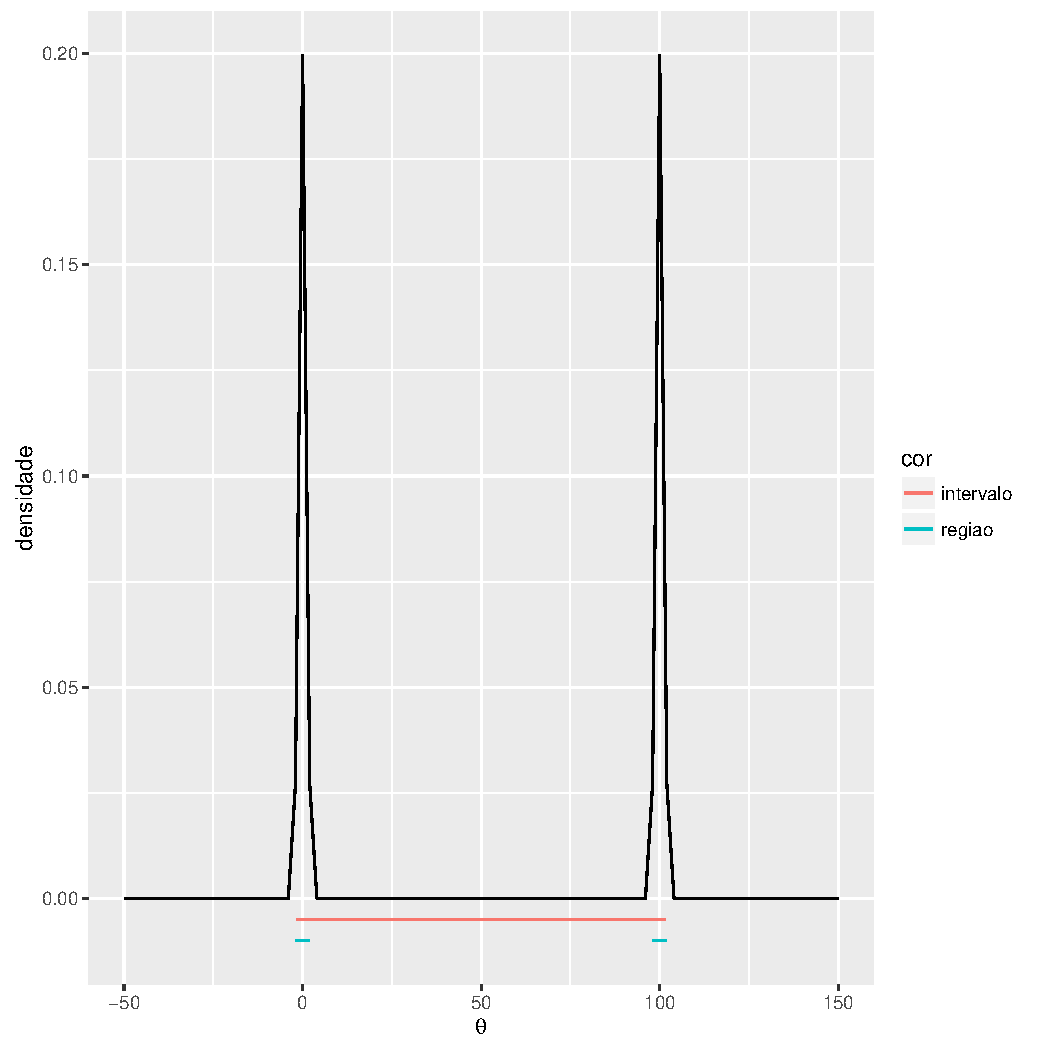
\includegraphics[scale=0.5]{chapter-decisions-normal-mixture.pdf}
 \caption{Densidade da mistura de 
 uma $N(0,1)$ e uma $N(100,1)$
 acompanhada de um intervalo de credibilidade e
 de uma região de credibilidade.}
 \label{figure:normal-mixture-1}
\end{figure}

Como uma alternativa a um 
intervalo de credibilidade,
poderíamos combinar um 
intervalo de credibilidade para cada 
uma das normais na mistura.
Sabemos que uma $N(0,1)$ tem 
probabilidade de $95\%$ de estar em $[-1.96,1.96]$.
Similarmente, a $N(100,1)$ tem 
probabilidade de $95\%$ de estar em $[98.04,101.96]$.
Assim, a mistura de 
uma $N(0,1)$ e uma $N(100,1)$ tem 
alta probabilidade de estar em 
$[-1.96,1.96] \cup [98.04,101.96]$.
Neste exemplo, intervalos são 
demasiadamente restritivos e 
não descrevem adequadamente 
a \emph{posteriori} multimodal.

Assim, nesta subseção consideraremos 
um problema de decisão em que,
ao invés de escolher um intervalo para 
descrever a posteriori,
é necessário escolher uma região para fazê-lo.
De forma geral, uma região pode ser 
qualquer subconjunto do espaço paramétrico.
Assim, temos que
$\mathcal{A}_{*} = \{R \subset \Theta\}$.
Para estudar este problema de decisão,
consideraremos a seguinte função de utilidade
\begin{align*}
 U(R(X),\theta)	
 &= \I(\theta \in R(X)) 
 -k\int_{x \in R(x)}{1 \cdot dx}
 & k > 0
\end{align*}
O elemento $\I(\theta \in R(X))$ indica que 
é desejável que $\theta$ esteja 
na região de credibilidade, $R(X)$.
Por outro lado,  $\int_{x \in R(x)}{dx}$ indica que
é desejável que a região $R(x)$ seja pequena, 
ou seja, tenha um volume pequeno.
\begin{theorem}
 \label{thm:hpd}
 Se $U(R(X),\theta)	= \I(\theta \in R(X)) - k\int_{x \in R(x)}{1 \cdot dx}$, então 
 a melhor região de credibilidade é tal que 
 $R(X) = \{\theta \in \Theta: f(\theta|X) \geq k\}$.
 Dizemos que $R(X)$ é um HPD (highest posterior density) 
 de $f(\theta|X)$.
\end{theorem}


\begin{definition}
Dizemos que uma região $R \subset \Theta$ tem credibilidade $1-\alpha$
se $\P(\theta \in R|\x)=1-\alpha$.
\end{definition}

\subsubsection*{Exercícios}

\begin{exercise}
 \label{ex:normal-credible}
 Dado $\mu$, $X_{1},\ldots,X_{n}$ são i.i.d. e 
 $X_{1} \sim N(\mu,1)$.
 \emph{A priori}, $\mu \sim N(0,1)$.
 \begin{enumerate}[label=(\alph*)]
  \item Ache um estimador para $\mu$ usando 
  cada utilidade que vimos em aula.
  \item Ache um intervalo para $\mu$ com 
  credibilidade $95\%$ para 
  cada utilidade que vimos em aula.
  \item Ache o HPD para $\mu$.
 \end{enumerate}
\end{exercise}

\solution{\textbf{Solução}:
 Decorre do \cref{ex:conjugate-normal-normal} que
 $\theta|X \sim N(\frac{n\bar{X}}{n+1},n+1)$.
 \begin{enumerate}[label=(\alph*)]
  \item Sabemos que, para a distância quadrática
  (\cref{thm:estimation_l2}), 
  o estimador ótimo é $E[\theta|X]$ e,
  para a distância em valor absoluto
  (\cref{thm:estimation_l1}), ele é $Med[\theta|X]$.
  Como a distribuição normal é 
  simétrica em torno da média, temos que 
  $Med[\theta|X] = E[\theta|X] = \frac{n\bar{X}}{n+1}$.
  
  \item \begin{itemize}
   \item Como a distribuição normal é unimodal,
   o intervalo de credibilidade pelo
   \cref{thm:credible_interval_1} é da forma 
   \begin{align*}
    [a,b] = \{\theta \in \Theta: f(\theta|X) \geq k\}
   \end{align*}
   Também, como a distribuição normal é 
   simétrica em torno de $\E[\theta|X]$ e unimodal,
   existe $c$ tal que
   \begin{align*}
    \{\theta \in \Theta: f(\theta|X) \geq k\} 
    &= [\E[\theta|X]-c,\E[\theta|X]+c]
   \end{align*}
   Assim, desejamos achar $c$ tal que
   \begin{align*}
    \P(\theta \in [\E[\theta|X]-c,\E[\theta|X]+c]|X)
    &= 95\%	\\
    \P\left(\frac{\theta
    -\E[\theta|X]}{\sqrt{\V[\theta|X]}} 
    \in \left[-\frac{c}{\sqrt{\V[\theta|X]}},
    \frac{c}{\sqrt{\V[\theta|X]}}\right]|X\right)	
    &= 95\%
   \end{align*}
   Como $\frac{\theta-\E[\theta|X]}{\V[\theta|X]}|X \sim N(0,1)$, $\frac{c}{\sqrt{\V[\theta|X]}}=1.96$.
   Como $\theta|X$ tem variância $(n+1)^{-1}$,
   obtemos o intervalo
   \begin{align*}
    \left[\frac{n\bar{X}}{n+1}-1.96(n+1)^{-0.5},
    \frac{n\bar{X}}{n+1}+1.96(n+1)^{-0.5}\right]
   \end{align*}
   
   \item Usando o \cref{thm:credible_interval_2}, 
   obtemos um intervalo $[a,b]$ tal que 
   $\P(\theta < a|X) = 2.5\%$ e 
   $\P(\theta > b|X) = 2.5\%$.
   \begin{align*}
    \P(\theta < a|X) &= 2.5\% \\
    \P\left(\frac{\theta-\E[\theta|X]}
    {\sqrt{\V[\theta|X}} 
    < \frac{a-\E[\theta|X]}{\sqrt{\V[\theta|X}}|X\right)
    &= 2.5\%
   \end{align*}
   Como $\frac{\theta-\E[\theta|X]}{\sqrt{\V[\theta|X]}}|X \sim N(0,1)$, 
   $\frac{a-\E[\theta|X]}{\sqrt{\V[\theta|X}}=-1.96$.
   Como a $\theta|X$ é simétrica em torno de
   $\E[\theta|X]$, 
   $\frac{b-\E[\theta|X]}{\sqrt{\V[\theta|X}}=1.96$.
   Assim, obtemos o intervalo
   \begin{align*}
    \left[\frac{n\bar{X}}{n+1}-1.96(n+1)^{-0.5},
    \frac{n\bar{X}}{n+1}+1.96(n+1)^{-0.5}\right]
   \end{align*}
   
   \item Usando o \cref{thm:credible_interval_3}, 
   obtemos um intervalo $[a,b]$ da forma
   \begin{align*}
    [a,b]
    &= \left[\E[\theta|X]-c\sqrt{\V[\theta|X]},
    \E[\theta|X]+c\sqrt{\V[\theta|X]}\right]
   \end{align*}
   Sabemos pelos itens anteriores que este 
   intervalo tem credibilidade $95\%$ somente se 
   $c=1.96$. Assim, obtemos o intervalo
   \begin{align*}
    \left[\frac{n\bar{X}}{n+1}-1.96(n+1)^{-0.5},
    \frac{n\bar{X}}{n+1}+1.96(n+1)^{-0.5}\right]
   \end{align*}
  \end{itemize}
  
  No caso da distribuição normal,
  que é unimodal e simétrica em torno de sua média,
  todos os intervalos de credibilidade são equivalentes.
	
  \item Como a distribuição a posteriori é unimodal,
  o HPD é equivalente ao intervalo de credibilidade 
  obtido no \cref{thm:credible_interval_1}.
  Assim, o HPD é
  \begin{align*}
   \left[\frac{n\bar{X}}{n+1}-1.96(n+1)^{-0.5},
   \frac{n\bar{X}}{n+1}+1.96(n+1)^{-0.5}\right]
  \end{align*}
 \end{enumerate}
}{}

\begin{exercise}
 Considere que $\theta|X \sim \text{Beta(0.05,0.05)}$.
 \begin{enumerate}[label=(\alph*)]
  \item $f(\theta|X)$ é uma função côncava?
  \item Use um \emph{software} estatístico para 
  achar um intervalo de credibilidade para $\theta|X$.
  \item Use um \emph{software} estatístico para 
  achar um HPD para $\theta|X$.
 \end{enumerate}
\end{exercise}

\solution{\textbf{Solução}:
 \begin{enumerate}[label=(\alph*)]
  \item Note que $f(\theta|X) = \beta^{-1}(0.05,0.05)\theta^{-0.95}(1-\theta)^{-0.95}$.
  A densidade a posteriori é indicada na  
  \cref{figure:bimodal-beta}.
  Note que $f(0|X) = f(1|X) = \infty$.
  Se $f$ é côncava, $a < b$ e $f(a) < f(b)$,
  então $f$ é decrescente a partir de $a$.
  Como $0 < 0.5 < 1$, 
  $f(0|X) > f(0.5|X)$ e 
  $f(0.5|X) < f(1|X)$,
  $f(\theta|X)$ não é côncava.	
  \begin{figure}
   \centering
   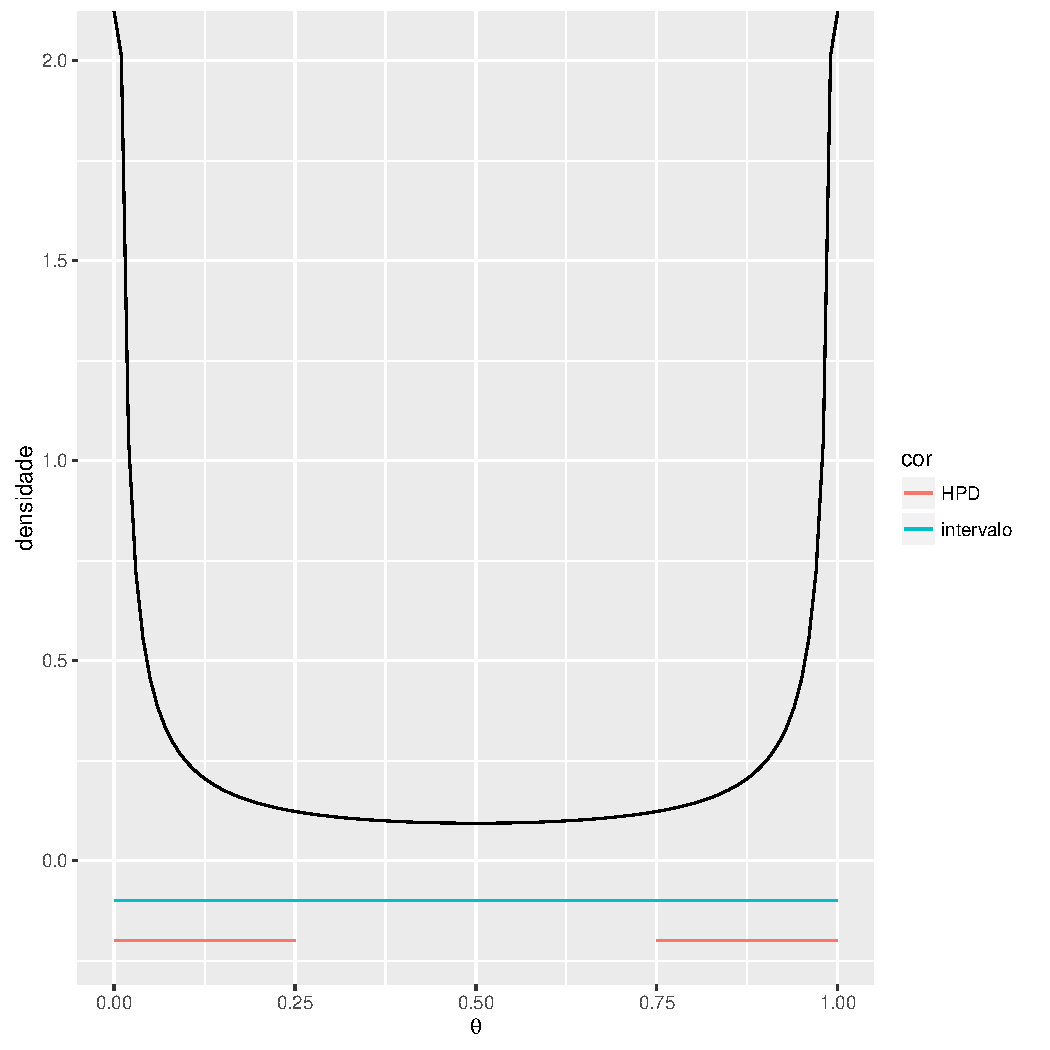
\includegraphics[scale=0.5]{chapter-decisions-bimodal-beta.pdf}
   \caption{Densidade da Beta$(0.05,0.05)$
   acompanhada de um intervalo de credibilidade 
   e o HPD.}
   \label{figure:bimodal-beta}
  \end{figure}
	
  \item Usando o \cref{thm:credible_interval_2},
  um possível intervalo de credibilidade, $[a,b]$,
  é tal que $\P(\theta < a|X) = 2.5\%$ e 
  $\P(\theta > b|X) = 2.5\%$.
  Podemos usar a função $qbeta$ no $R$ para
  obter os percentis da Beta$(0.05,0.05)$.
  O $R$ indica que eles são $8.8e-27$ e $1$.
  Portanto, o intervalo de credibilidade é
  praticamente o intervalo $[0,1]$ inteiro.

  \item Note pela \cref{figure:bimodal-beta} que 
  as regiões de maior densidade são
  os valores extremos à esquerda e à direita.
  Portanto, o HPD é composto por estes extremos.
  Como a distribuição a posteriori é simétrica em 
  torno de $0.5$,
  O HPD pode ser obtido determinando 
  $\P(\theta < a|X) = 47.5\%$ e
  $\P(\theta > b|X) = 52.5\%$.
  O HPD será $[0,a] \cup [b,1]$.
  Usando o $R$ encontramos que 
  $a \approx 0.25$ e $b \approx 0.75$.
 \end{enumerate}
}{}

\begin{exercise}[Sugestão de Aline Tonon]
 Considere o problema de determinar um intervalo de credibilidade, $(a,b)$, com a função de utilidade, $U((a,b),\theta)=\frac{\I(\theta \in (a,b))}{b-a}$. Prove que, se $(a^*,b^*)$ é um intervalo de credibilidade ótimo, então $f_{\theta|X}(a^*|X)=f_{\theta|X}(b^*|X)$.
\end{exercise}

\solution{\textbf{Solução}: Defina
 \begin{align*}
  g(a,b) := \E\left[U((a,b),\theta)|X\right]
  &= \E\left[\frac{\I(\theta \in (a,b))}{b-a}\bigg|X\right]
  = \frac{F_{\theta|X}(b|X)-F_{\theta|X}(a|X)}{b-a}
 \end{align*}
 Para que um ponto $(a,b)$ maximize $g(a,b)$,
 ele deve ser tal que $\nabla g(a,b)=\textbf{0}$.
 Note que
 \begin{align*}
  \nabla g(a,b) &= \left(\frac{\partial \frac{F_{\theta|X}(b|X)-F_{\theta|X}(a|X)}{b-a}}{\partial a}, \frac{\partial \frac{F_{\theta|X}(b|X)-F_{\theta|X}(a|X)}{b-a}}{\partial b}\right) \\
  &= \left(-\frac{f_{\theta|X}(a|X)(b-a)+(F_{\theta|X}(b|X)-F_{\theta|X}(a|X))}{(b-a)^2}, \frac{f_{\theta|X}(b|X)(b-a)-(F_{\theta|X}(b|X)-F_{\theta|X}(a|X))}{(b-a)^2} \right)
 \end{align*}
 Portanto, para que $\nabla g(a,b) = \textbf{0}$,
 obtemos
 \begin{align*}
  \begin{cases}
   f_{\theta|X}(a|X) = \frac{F_{\theta|X}(b|X)-F_{\theta|X}(a|X)}{b-a} \\
   f_{\theta|X}(b|X) = \frac{F_{\theta|X}(b|X)-F_{\theta|X}(a|X)}{b-a}
  \end{cases}
 \end{align*}
 Conclua que, se $(a^*,b^*)$ maximiza 
 a utilidade esperada, então
 $f_{\theta|X}(a^*|X)=f_{\theta|X}(b^*|X)$.
}{}

\begin{exercise}
 Considere o problema de determinar um intervalo de credibilidade, $(a,b)$, com a função de utilidade, $U((a,b),\theta)=\frac{k-(a-\theta)_{+}-(b-\theta)_{+}}{b-a}$. Prove que, se $(a^*,b^*)$ é um intervalo de credibilidade ótimo, então
 $F_{\theta|X}(a^*|X)=1-F_{\theta|X}(b^*|X)$.
\end{exercise}

\solution{\textbf{Solução}: Defina
 \begin{align*}
  g(a,b) := \E\left[U((a,b),\theta)|X\right]
  &= \E\left[\frac{k-(a-\theta)_{+}-(b-\theta)_{+}}{b-a}\bigg|X\right] \\
  &= \frac{k-\int_{-\infty}^{a}{(a-\theta)f_{\theta|X}(t|X)dt} -\int_{b}^{\infty}{(\theta-b)f_{\theta|X}(t|X)dt}}{b-a}
 \end{align*}
 Defina $h(a,b) := k-\int_{-\infty}^{a}{(a-\theta)f_{\theta|X}(t|X)dt} -\int_{b}^{\infty}{(\theta-b)f_{\theta|X}(t|X)dt}$.
 Para que um ponto $(a,b)$ maximize $g(a,b)$,
 ele deve ser tal que $\nabla g(a,b)=\textbf{0}$.
 Note que
 \begin{align*}
  \nabla g(a,b) &= \left(\frac{\partial g(a,b)}{\partial a}, \frac{\partial g(a,b)}{\partial b}\right) \\
  &= \left(\frac{-(b-a)\int_{-\infty}^{a}{f_{\theta|X}(t|X)dt} + h(a,b)}{(b-a)^2}, \frac{(b-a)\int_{b}^{\infty}{f_{\theta|X}(t|X)dt}-h(a,b)}{(b-a)^2} \right)
 \end{align*}
 Portanto, para que $\nabla g(a,b) = \textbf{0}$,
 é necessário que
 \begin{align*}
  \begin{cases}
   \int_{\infty}^{a}{f_{\theta|X}(t|X)dt} = 
   \frac{h(a,b)}{b-a}\\
   \int_{b}^{\infty}{f_{\theta|X}(t|X)dt} = 
   \frac{h(a,b)}{b-a}
  \end{cases}
 \end{align*}
 Conclua que, se $(a^*,b^*)$ maximiza a
 utilidade esperada, então
 $\int_{\infty}^{a^*}{f_{\theta|X}(t|X)dt}=\int_{b^*}^{\infty}{f_{\theta|X}(t|X)dt}$,
 isto é, 
 $F_{\theta|X}(a^*|X)=1-F_{\theta|X}(b^*|X)$.
}{}


\include{chapters/07-3-inference-hypothesis}
\include{chapters/07-4-likelihood-principle}
\include{chapters/08-review-2}

\section{Estatística Bayesiana Computacional}

Até o momento, trabalhamos com modelos tais que
era possível calcular analiticamente 
a distribuição a posteriori para o parâmetro do
modelo estatístico. Para tal, usamos a expressão
obtida a partir do Teorema de Bayes:
\begin{align*}
 f(\theta|x)
 &= \frac{f(\theta)f(x|\theta)}
 {\int{f(\theta)f(x|\theta)d\theta}}
\end{align*}

Contudo, geralmente não é possível calcular diretamente
$\int{f(\theta)f(x|\theta)d\theta}$
ou aproximar esta expressão por métodos determinísticos de
integração (especialmente se o parâmetro tiver
alta dimensionalidade). Assim, para
realizar uma análise Bayesiana, é necessário
desenvolver outras maneiras de avaliar a posteriori.

\subsection{Método de Monte Carlo}

Seja $g$ uma função de $\theta$, e assuma que desejamos aproximar
$\E[g(\theta)|x]$. Por exemplo, podemos estar interessados em aproximar
$\E[\theta|x]$.
Considere que, de alguma forma, obtivemos uma
amostra i.i.d. da posteriori de $\theta$, $f(\theta|x)$.
Denotaremos esta amostra por $T_{1},\ldots,T_{B}$.
\begin{align*}
 \E[g(T_{i})]
 &= \int{g(t)f(t|x)dt}
 & \text{$T_{i}$ tem distribuição $f(t|x)$} \\
 &= \int{g(\theta)f(\theta|x)d\theta}
 = \E[g(\theta)|x]
\end{align*}
Portanto, como $T_{1},\ldots,T_{B}$ é uma amostra i.i.d.,
decorre da Lei dos Grandes Números que, se
$B$ for suficientemente grande, então
\begin{align}
 \label{eqn:monte_carlo_1}
 \hat{\E}[g(\theta)|x]
 := \frac{\sum_{i=1}^{B}{g(T_{i})}}{B}
 \approx \E[g(\theta)|x].
\end{align}

Assim, para estimar $\E[g(\theta)|x]$, basta
(i) obter uma amostra i.i.d. da distribuição a posteriori e
(ii) calcular a média dos $g(T_{i})$'s. 


Além disso, se $\V[g(\theta)|x] < \infty$, então
decorre do Teorema do Limite Central que
\begin{align}
 \label{eqn:monte_carlo_3}
 \frac{\hat{E}[g(\theta)|x]-\E[g(\theta)|x]}{\sqrt{B}}
 \approx N(0,\sqrt{B}^{-1}\V[g(\theta)|x])
\end{align}
Assim, se $\psi$ é a função de distribuição acumulada da
$N(0,1)$, então decorre das
\cref{eqn:monte_carlo_2,eqn:monte_carlo_3} que
\begin{align}
 \label{eqn:monte_carlo_4}
 \left[\hat{\E}[g(\theta)|x]
 +\psi^{-1}(0.5\alpha)\sqrt{B^{-1}\hat{\V}[g(\theta)|x]},
 \hat{\E}[g(\theta)|x]
 +\psi^{-1}(1-0.5\alpha)
 \sqrt{B^{-1}\hat{\V}[g(\theta)|x]}\right]
\end{align}
é um intervalo de confiança aproximadamente
$1-\alpha$ para $\E[g(\theta)|x]$.
Note que decorre da
\cref{eqn:monte_carlo_1} que
$\frac{\sum_{i=1}^{n}{g(T_{i})^{2}}}{B} \approx \E[g(\theta)^{2}|x]$.
Portanto, como podemos escrever
$\V[g(\theta)|x]$ como
$\E[g(\theta)^{2}|x]-\E[g(\theta)|x]^{2}$, então a variância de 
$g(\theta)$ pode ser aproximada como
\begin{align}
 \label{eqn:monte_carlo_2}
 \hat{\V}[g(\theta)|x]
 := \frac{\sum_{i=1}^{B}{g(T_{i})^{2}}}{B}
 -\left(\frac{\sum_{i=1}^{B}{g(T_{i})}}{B}\right)^{2}
 \approx \V[g(\theta)|x].
\end{align}


Assim,
\begin{theorem}[Monte Carlo]
 \label{thm:monte_carlo}
 Se $T_{1},\ldots,T_{B}$ é uma amostra i.i.d. de 
 $f(\theta|x)$ e $g$ é uma função arbitrária, então
 $\hat{\E}[g(\theta)|x]$ aproxima $\E[g(\theta|x)]$ e 
 um intervalo de confiança aproximadamente $1-\alpha$ para
 $\E[g(\theta)|x]$ é
 \begin{align*}
  \left[\hat{\E}[g(\theta)|x]
  +\psi^{-1}(0.5\alpha)\sqrt{B^{-1}\hat{\V}[g(\theta)|x]},
  \hat{\E}[g(\theta)|x]+\psi^{-1}(1-0.5\alpha)
  \sqrt{B^{-1}\hat{\V}[g(\theta)|x]}\right]
 \end{align*}
\end{theorem}

Observe que o \cref{thm:monte_carlo} permite aproximar
e avaliar o erro de aproximação para
diversas quantidades importantes de $f(\theta|x)$.
Por exemplo, tomando $g(\theta) = \theta^{n}$,
é possível aproximar $\E[\theta^{n}|x]$.
Similarmente, se $R \subset \theta$ e
$g(\theta) = \I(\theta \in R)$,
então é possível aproximar 
$\E[g(\theta)] = \P(\theta \in R)$.
Podemos usar o seguinte código para implementar o \cref{thm:monte_carlo} em R

\begin{algorithm2}[Monte Carlo] \
 \label{algo:monte_carlo}
\begin{knitrout}
\definecolor{shadecolor}{rgb}{0.969, 0.969, 0.969}\color{fgcolor}\begin{kframe}
\begin{alltt}
\hlcom{####################################################################}
\hlcom{## amostrador: funcao usada para obter a amostra do Monte Carlo,  ##}
\hlcom{## deve retornar uma lista de amostras                            ##}
\hlcom{## B: tamanho da amostra gerada.                                  ##}
\hlcom{## g: funcao cujo valor esperado estamos interessados.            ##}
\hlcom{## retorna: amostra de Monte Carlo e algumas de suas estatisticas ##}
\hlcom{####################################################################}
\hlstd{monte_carlo} \hlkwb{<-} \hlkwa{function}\hlstd{(}\hlkwc{amostrador}\hlstd{,} \hlkwc{B}\hlstd{,} \hlkwc{g}\hlstd{,} \hlkwc{...}\hlstd{)}
\hlstd{\{}
 \hlstd{amostra} \hlkwb{<-} \hlkwd{amostrador}\hlstd{(B, ...)}
 \hlstd{amostra_g} \hlkwb{<-} \hlkwd{sapply}\hlstd{(amostra, g)} \hlcom{#obtem g(x) para cada x em amostra}
 \hlstd{est_g} \hlkwb{<-} \hlkwd{mean}\hlstd{(amostra_g)}
 \hlstd{var_g} \hlkwb{<-} \hlkwd{var}\hlstd{(amostra_g)}
 \hlkwd{return}\hlstd{(}\hlkwd{list}\hlstd{(}\hlkwc{amostra}\hlstd{=amostra,}
             \hlkwc{estimador}\hlstd{=est_g,}
             \hlkwc{ic}\hlstd{=}\hlkwd{c}\hlstd{(est_g}\hlopt{+}\hlkwd{qnorm}\hlstd{(}\hlnum{0.025}\hlstd{)}\hlopt{*}\hlkwd{sqrt}\hlstd{(var_g}\hlopt{/}\hlstd{B),}
                  \hlstd{est_g}\hlopt{+}\hlkwd{qnorm}\hlstd{(}\hlnum{0.975}\hlstd{)}\hlopt{*}\hlkwd{sqrt}\hlstd{(var_g}\hlopt{/}\hlstd{B))}
       \hlstd{))}
\hlstd{\}}
\end{alltt}
\end{kframe}
\end{knitrout}
\end{algorithm2}

Assim, utilizando o método de Monte Carlo,
podemos obter diversas características relevantes da
posteriori a partir de uma amostra desta.
A pergunta que resta é: como obter uma
amostra de $f(\theta|x)$ quando não conseguimos
calcular esta quantidade analiticamente?

\subsubsection{O método da rejeição}

O método da rejeição pode ser empregado
para obter uma amostra da posteriori.
Ele pode ser descrito nos seguinte passos:

\begin{enumerate}
 \item Considere que $f(\theta)$ é a
 densidade da qual você quer simular e
 $\tilde{f}(\theta) \propto f(\theta)$
 \item Ache uma densidade, $h(\theta)$ e
 uma constante, $M$, tais que
 $\tilde{f}(\theta) \leq M h(\theta)$.
 \item Gere uma proposta, $T$, de $h(\theta)$.
 \item Gere $U \sim \text{Uniforme}(0,1)$.
 \item Se $U \leq \frac{\tilde{f}(T)}{Mh(T)}$, então
 retorne $T$ como sua amostra.
 Caso contrário, retorne ao passo 3.
\end{enumerate}

Código genérico para o método da rejeição
é apresentado no \cref{algo:rejection}, abaixo.

\begin{algorithm2}[Método da rejeição] \
 \label{algo:rejection}
\begin{knitrout}
\definecolor{shadecolor}{rgb}{0.969, 0.969, 0.969}\color{fgcolor}\begin{kframe}
\begin{alltt}
\hlcom{#############################################################################}
\hlcom{## Código ilustrativo em R para o método da rejeição.                      ##}
\hlcom{## B: tamanho da amostra a ser gerada                                      ##}
\hlcom{## pf.avaliar: calcula o valor de uma função proporcional a f.             ##}
\hlcom{## h.avaliar: calcula o valor da densidade h.                              ##}
\hlcom{## h.gerar: gera uma variável aleatória com densidade h.                   ##}
\hlcom{## M: a constante usada no método da rejeição.                             ##}
\hlcom{## retorna: uma variável aleatória de densidade proporcional a pf.avaliar. ##}
\hlcom{#############################################################################}
\hlstd{amostrador_rejeicao} \hlkwb{<-} \hlkwa{function}\hlstd{(}\hlkwc{B}\hlstd{,} \hlkwc{pf.avaliar}\hlstd{,} \hlkwc{h.avaliar}\hlstd{,} \hlkwc{h.gerar}\hlstd{,} \hlkwc{M}\hlstd{)}
\hlstd{\{}
 \hlstd{amostra} \hlkwb{<-} \hlkwd{vector}\hlstd{(}\hlkwc{mode}\hlstd{=}\hlstr{"list"}\hlstd{,} \hlkwc{length}\hlstd{=B)}
 \hlkwa{for}\hlstd{(ii} \hlkwa{in} \hlnum{1}\hlopt{:}\hlstd{B)}
 \hlstd{\{}
  \hlstd{T} \hlkwb{<-} \hlkwd{h.gerar}\hlstd{()}
  \hlkwa{while}\hlstd{(}\hlkwd{runif}\hlstd{(}\hlnum{1}\hlstd{,}\hlnum{0}\hlstd{,}\hlnum{1}\hlstd{)} \hlopt{>} \hlkwd{pf.avaliar}\hlstd{(T)}\hlopt{/}\hlstd{(M}\hlopt{*}\hlkwd{h.avaliar}\hlstd{(T)))}
  \hlstd{\{}
   \hlstd{T} \hlkwb{<-} \hlkwd{h.gerar}\hlstd{()}
  \hlstd{\}}
  \hlstd{amostra[[ii]]} \hlkwb{<-} \hlstd{T}
        \hlstd{\}}
 \hlkwd{return}\hlstd{(amostra)}
\hlstd{\}}
\end{alltt}
\end{kframe}
\end{knitrout}
\end{algorithm2}

\begin{example}
 \label{ex:rejection-circle}
 Considere que você deseja simular de uma 
 distribuição uniforme num círculo de
 raio centrado na origem.
 Os passos do método da rejeição são os seguintes:
 \begin{enumerate}
  \item Neste caso, $f(\theta) = \pi^{-1} (\theta_{1}^{2}+\theta_{1}^{2} \leq 1)$.
  Podemos tomar $\tilde{f}(\theta) =(\theta_{1}^{2}+\theta_{1}^{2} \leq 1)$, ou seja,
  $\tilde{f}(\theta) = \pi f(\theta)$.
  \item Considere que você é capaz de simular de uma
  uniforme num quadrado de lado $2$ centrado na origem.
  Neste caso, $h(\theta) = 4^{-1}\I(|\theta_{1}| \leq 1, |\theta_{2}| \leq 1)$.
  Note que $\tilde{f}(\theta) \leq 4h(\theta)$.
  Portanto, podemos tomar $M=4$.
  Finalmente $\frac{\tilde{f}(\theta)}{4h(\theta)} = \tilde{f}(\theta)$.
  \item Geramos $T_{1}$ e $T_{2}$ com densidade $h(\theta)$.
  \item Geramos $U \sim \text{Uniforme}(0,1)$.
  \item Se $T_{1}^{2} + T_{1}^{2} \leq 1$, então
  $\frac{\tilde{f}(\theta)}{4h(\theta)} = \tilde{f}(\theta) = 1$.
  Assim, para qualquer $U$ gerado, retornaremos $T$.
  Se $T_{1}^{2} + T_{1}^{2} > 1$, então
  $\frac{\tilde{f}(\theta)}{4h(\theta)} = \tilde{f}(\theta) = 0$.
  Assim, para qualquer $U$ gerado,
  retornaremos ao passo 3.
  Note que, neste caso, sequer precisaríamos ter
  gerado $U$.
 \end{enumerate}
 Podemos descrever o algoritmo acima utilizando o
 seguinte código em $R$.

\begin{knitrout}
\definecolor{shadecolor}{rgb}{0.969, 0.969, 0.969}\color{fgcolor}\begin{kframe}
\begin{alltt}
\hlcom{#######################################################}
\hlcom{## retorna: uma variável aleatória de densidade      ##}
\hlcom{## uniforme no círculo de raio 1 e centro na origem. ##}
\hlcom{#######################################################}
\hlstd{B} \hlkwb{=} \hlnum{100}
\hlstd{h.gerar} \hlkwb{=} \hlkwa{function}\hlstd{()} \hlkwd{runif}\hlstd{(}\hlnum{2}\hlstd{,}\hlopt{-}\hlnum{1}\hlstd{,}\hlnum{1}\hlstd{)}
\hlstd{h.avaliar} \hlkwb{=} \hlkwa{function}\hlstd{(}\hlkwc{x}\hlstd{) ((x[}\hlnum{1}\hlstd{]}\hlopt{^}\hlnum{2} \hlopt{<=} \hlnum{1}\hlstd{)} \hlopt{&} \hlstd{(x[}\hlnum{2}\hlstd{]}\hlopt{^}\hlnum{2} \hlopt{<=} \hlnum{1}\hlstd{))}\hlopt{/}\hlnum{4}
\hlstd{pf.avaliar} \hlkwb{=} \hlkwa{function}\hlstd{(}\hlkwc{x}\hlstd{) (x[}\hlnum{1}\hlstd{]}\hlopt{^}\hlnum{2} \hlopt{+} \hlstd{x[}\hlnum{2}\hlstd{]}\hlopt{^}\hlnum{2} \hlopt{<=} \hlnum{1}\hlstd{)}\hlopt{/}\hlstd{pi}
\hlstd{M} \hlkwb{=} \hlnum{4}\hlopt{/}\hlstd{pi}
\hlstd{dados} \hlkwb{=} \hlkwd{amostrador_rejeicao}\hlstd{(B, pf.avaliar, h.avaliar, h.gerar, M)}
\end{alltt}
\end{kframe}
\end{knitrout}

 O funcionamento do algoritmo acima é ilustrado na
 \cref{fig:rejection-circle}.
 Os pontos indicam as $2000$ propostas que foram
 geradas para obter uma amostra de tamanho $1586$.
 Dentre estes pontos, os vermelhos foram aceitos e
 os azuis foram rejeitados.
 Neste caso, aproximadamente 80\% dos pontos
 foram aceitos. Observe que pontos rejeitados são
 um desperdício computacional, dado que
 recursos são gastos para gerá-los, mas eles não
 fazem parte da amostra gerada.
 Neste sentido, gerar propostas de
 figuras geométricas mais próximas ao círculo
 diminuirá a rejeição e, portanto, a princípio,
 aumentará o rendimento do algoritmo.
 A dificuldade neste sentido é criar métodos para
 gerar propostas de  outras figuras geométricas de
 forma tão eficiente quanto do quadrado.
 \begin{figure}
  \centering
  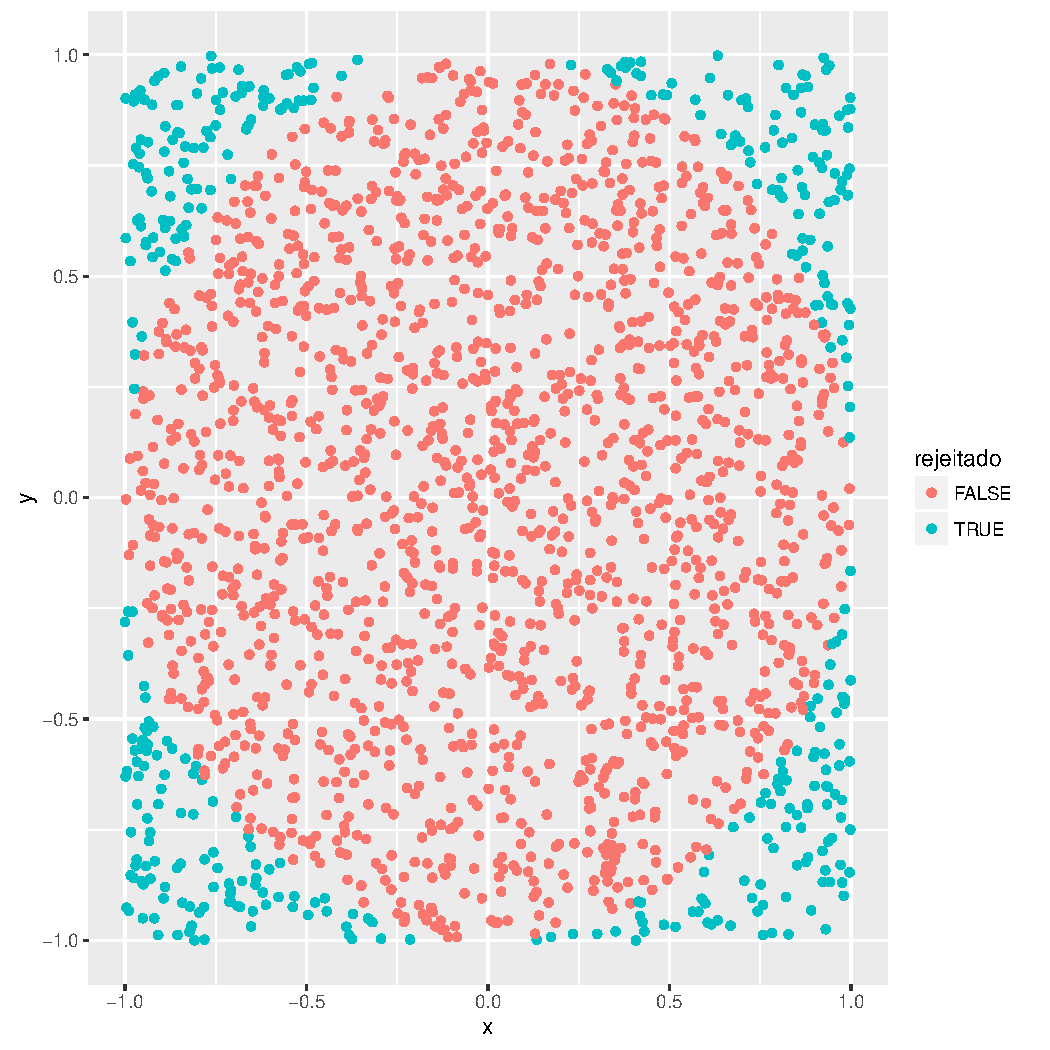
\includegraphics[scale=0.5]{chapter-computing-rejection-circle}
  \caption{Amostra de $2000$ propostas geradas pelo
  método da rejeição descrito
  no \cref{ex:rejection-circle}.}
  \label{fig:rejection-circle}
 \end{figure}
\end{example}

\begin{example}
 \label{ex:rejection-beta-2-2}
 Você deseja simular da densidade
 $f(\theta) = 6\theta(1-\theta)\I(\theta \in (0,1))$.
 Note que $f(\theta)$ é a densidade da Beta$(2,2)$.
 Podemos tomar, por exemplo,
 $\tilde{f}(\theta) = \theta(1-\theta) \I(\theta \in (0,1))$.
 Assim, $\tilde{f}(\theta) \leq 0.25 \I(\theta \in (0,1)) = 0.25 \cdot h(\theta)$,
 onde $h(\theta)$ é a densidade da
 Uniforme$(0,1)$ e $M=0.25$.
 Note que $\frac{\tilde{f}(\theta)}{M h(\theta)} = 4\theta(1-\theta)$.
 Portanto, é possível simular de $f$ pelo
 método da rejeição 
 usando o seguinte código
 \begin{verbatim}
###############################################################
## retorna: uma variável aleatória de distribuição Beta(2,2) ##
###############################################################
simula_beta_2_2_rejeicao <- function(B)
{
 amostra <- vector(mode="list", length=B)
 for(ii in 1:B)
 {
  T <- runif(1)
  while(runif(1) > 4*T*(1-T)) T <- runif(1)
  amostra[[ii]] <- T
 }
 return(amostra)
}
\end{verbatim}

 O funcionamento do algoritmo acima é ilustrado na
 \cref{fig:rejection-beta-2-2}.
 O eixo $x$ dos pontos indicam as $2000$ propostas que
 foram geradas para obter uma amostra de tamanho $1315$.
 O eixo $y$ dos pontos indicam as
 variáveis aleatórias uniformes geradas para
 determinar se as propostas eram rejeitadas.
 Dentre os pontos gerados, os vermelhos foram aceitos e
 os azuis foram rejeitados.
 Note que, como $\frac{\tilde{f}(\theta)}{h(\theta)} = 4\theta(1-\theta)$,
 $T$ era rejeitado se $U > 4T(1-T)$.
 A \cref{fig:rejection-beta-2-2} também ilustra um
 outro aspecto do método da rejeição.
 Ao combinarmos $T$ e $U$, obtemos uma
 distribuição uniforme em $[0,1]^{2}$.
 Ao remover, os pontos azuis,
 os pontos vermelhos que restam distribuem-se de
 acordo com uma distribuição Beta(2,2) no eixo $x$.
 \begin{figure}
  \centering
  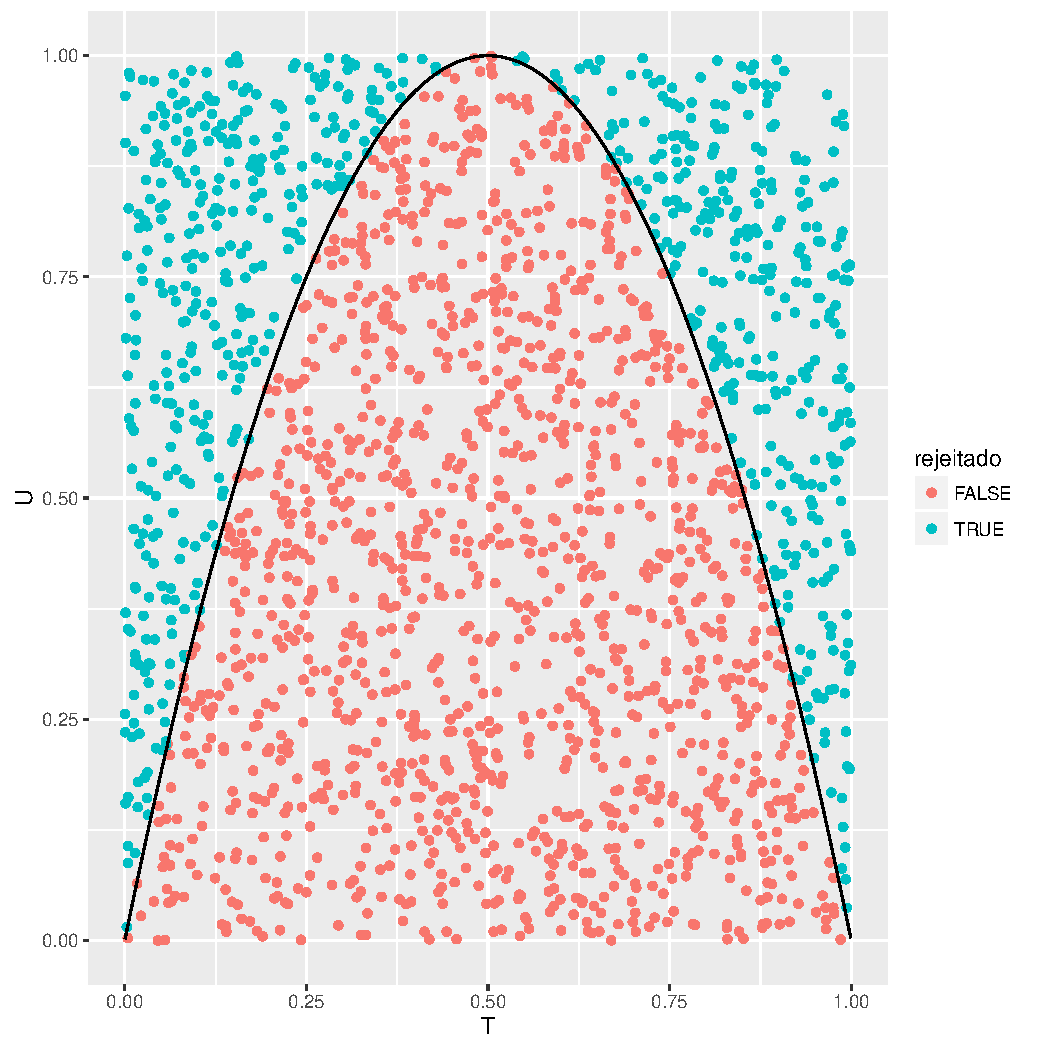
\includegraphics[scale=0.5]{chapter-computing-rejection-beta-2-2}
  \caption{Amostra de $2000$ propostas geradas pelo
  método da rejeição descrito no
  \cref{ex:rejection-beta-2-2}.}
  \label{fig:rejection-beta-2-2}
 \end{figure}
\end{example}

\begin{theorem}
 Se $\theta$ foi gerado de acordo com o
 método da rejeição usando as funções $f(\theta)$,
 $\tilde{f}(\theta)$, $h(\theta)$ e $M$
 conforme a descrição no início deste capítulo,
 então $\theta$ tem distribuição com densidade $f$.
\end{theorem}

\begin{proof}
 Considere que $N$ é o número de propostas geradas
 até a primeira aceitação, que
 $T_{1},\ldots,T_{i},\ldots$ é um conjunto de propostas e
 $U_{1},\ldots,U_{i},\ldots$ é um conjunto de uniformes.
 Note que $A_{i} = \I\left(U_{i} \leq \frac{\tilde{f}(T_{i})}{Mh(T_{i})}\right)$ são i.i.d. e
 \begin{align*}
  \P\left(U_{i} \leq
  \frac{\tilde{f}(T_{i})}
  {Mh(T_{i})}\right)
  &= \int_{-\infty}^{\infty}
  {\frac{\tilde{f}(t)}{Mh(t)} h(t) dt} \\
  &= M^{-1}\int_{-\infty}^{\infty}
  {\tilde{f}(t)dt} := p_{1}
 \end{align*}
 Portanto, como $N = \min\left(i: \I(U_{i} \leq \frac{\tilde{f}(T_{i})}{Mh(T_{i})}) =1\right)$,
 então $N \sim \text{Geométrica}(p_{1})$. Assim, para todo 
 $B \subset \mathbb{R}$,
 \begin{align*}
  \P(\theta \in B)
  &= \sum_{n}{\P(\theta \in B, N = n)} \\
  &= \sum_{n}{\P(\cap_{i=1}^{n-1}{A_{i}^{c}} \cap (A_{n} \cap T_{n} \in B))} \\
  &= \sum_{n}{\P(\cap_{i=1}^{n-1}{A_{i}^{c}})\P(A_{n} \cap T_{n} \in B)} \\
  &= \sum_{n}{(1-p_{1})^{n-1}\int_{B}{\frac{\tilde{f}(t)}{Mh(t)} h(t)dt}} \\
  &= \int_{B}{M^{-1}\tilde{f}(t)dt}\sum_{n}{(1-p_{1})^{n-1}} \\
  &= \frac{\int_{B}{M^{-1}\tilde{f}(t)dt}}{p_{1}} \\
  &= \frac{M^{-1}\int_{B}{\tilde{f}(t)dt}}{M^{-1}\int_{-\infty}^{\infty}{\tilde{f}(t)dt}} \\
  &= \int_{B}{\frac{\tilde{f}(t)}{\int_{-\infty}^{\infty}{\tilde{f}(t)dt}}dt} \\
  &= \int_{B}{f(t)dt}
 \end{align*} 
\end{proof}

\subsubsection*{Exercícios}

\begin{exercise}
 No \cref{ex:rejection-circle},
 usamos propostas de um quadrado de lado $2$
 e centro na origem.
 Poderíamos ter implementado o algoritmo da rejeição
 usando propostas de um quadrado de lado $1$?
 E de um quadrado de lado $3$?
 Esboce estas três figuras acompanhadas
 do círculo de raio $1$ e centro na origem.
 Compare as propostas sugeridas em relação à sua eficiência computacional.
\end{exercise}

\solution{\textbf{Solução}: A densidade de uma
 distribuição uniforme no quadrado de lado $1$ e
 centro na origem é,
 $h_{1}(\theta) := \I(|\theta_{1}| \leq 0.5, |\theta_{2}| \leq 0.5)$.
 Se tomarmos $f(\theta)$ como a densidade da
 distribuição uniforme no círculo de raio $1$ e
 centro na origem, então $f((1,0)) = 1$ e
 $h_{1}((1,0))$. Portanto, não existe $M > 0$ tal que
 $f((1,0)) \leq Mh_{1}((1,0))$.
														  Assim, não é possível usar o método da rejeição para  simular de $f$ a partir de $h_{1}$. 
 Por outro outro lado, defina
 $h_{2} = 4^{-1}\I(|\theta_{1}|\leq 1, |\theta_{2}|\leq 1)$ e $h_{3} = 9^{-1}\I(|\theta_{1}|\leq 1.5, |\theta_{2}|\leq 1.5)$ como as densidades dos quadrados
 de lado $2$ e $3$, e $\tilde{f}(\theta) = \I(\theta_{1}^{2}+\theta_{2}^{2} \leq 1)$.
 Note que $\tilde{f}(\theta) \leq 4 h_{2}$ e
 $\tilde{f}(\theta) \leq 9 h_{3}$.
 Assim, a probabilidade de aceitação usando
 $\tilde{f}$, $h_{2}$ e $M=4$ é dada por
 
 \begin{align*}
  \P\left(U \leq \frac{\tilde{f}(T)}{4 h_{2}(T)}\right)
  &= \int_{-\infty}^{\infty}{\frac{\tilde{f}(t)}{4 h_{2}(t)} h_{2}(t)dt} \\
  &= 4^{-1}\int_{-\infty}^{\infty}{\tilde{f}(t)dt}
  = \frac{\pi}{4}
 \end{align*}
 
 Similarmente, a probabilidade de aceitação usando
 $\tilde{f}$, $h_{3}$ e $M=9$ é $\frac{\pi}{9}$.
 Como a probabilidade de aceitação usando $h_{2}$ é
 maior do que usando $h_{3}$, o primeiro é
 mais computacionalmente eficiente.
 
 Este argumento é ilustrado pela
 \cref{fig:rejection-squares}.
 Note que a região de rejeição usando
 $h_{3}$ (azul e verde) é consideravelmente maior
 que aquela usando $h_{2}$ (verde).
 \begin{figure}
  \centering
  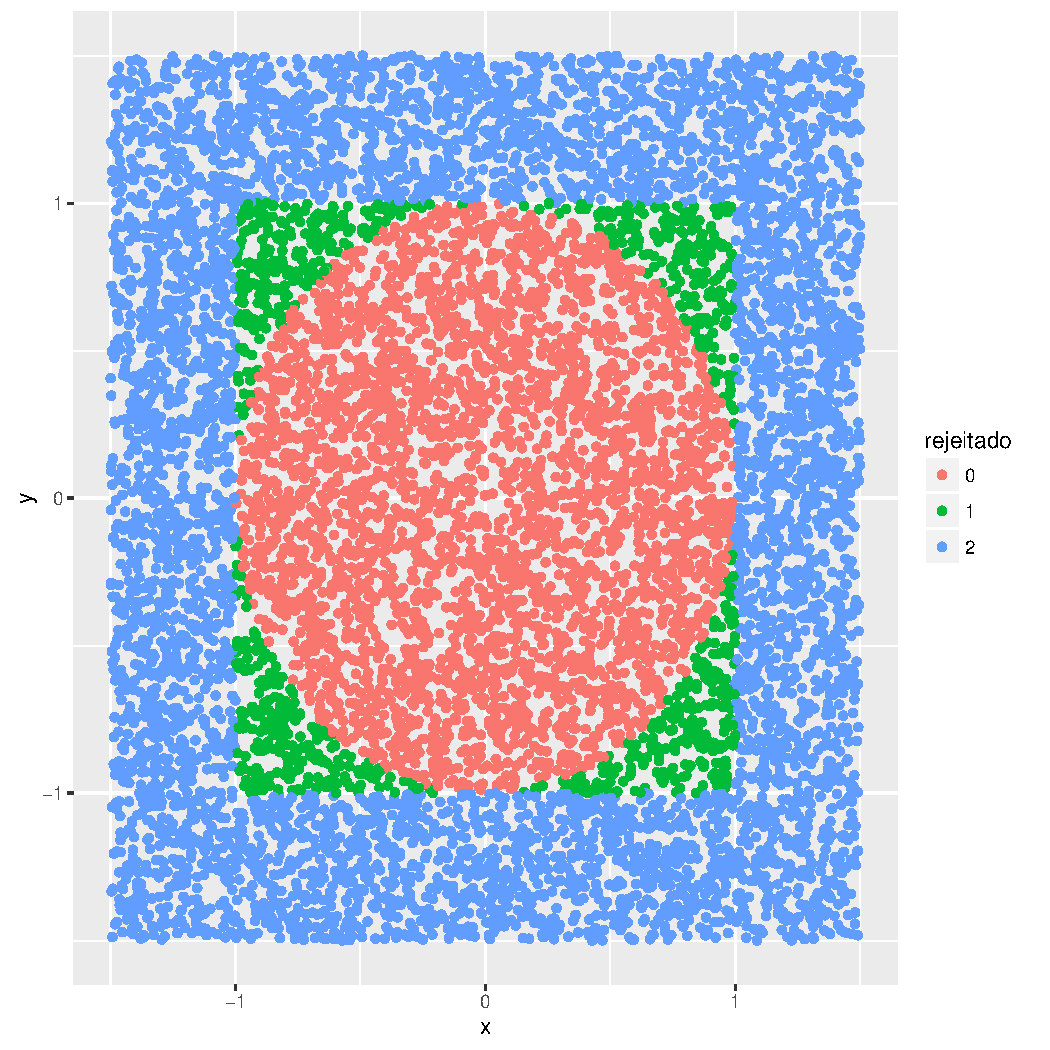
\includegraphics[scale=0.5]{chapter-computing-rejection-squares}
  \caption{Ilustração das regiões de rejeição
  para propostas de $h_{2}$ (verde) e de
  $h_{3}$ (verde e azul).}
  \label{fig:rejection-squares}
 \end{figure}
}{}

\begin{exercise}
 Escreva um código para
 simular de distribuição uniforme
 em uma esfera de raio $1$ e centro $0$.
 Use o Método de Monte Carlo para estimar
 a distância média de de um ponto amostrado à origem.
\end{exercise}

\cprotect \solution{
 \textbf{Solução}: Podemos escolher
 $\tilde{f}(\theta) = \I(\theta_{1}^{2}+\theta_{2}^{2}+\theta_{3}^{2} \leq 1)$.
 Se usarmos como propostas a uniforme no cubo de
 aresta $1$ e centro na origem, então
 $h(\theta) = 8^{-1}\I(|\theta_{i}| \leq 1, i \in \{1,2,3\})$.
 Assim, $\tilde{f}(\theta) \leq 8h(\theta)$ e
 tomamos $M=8$.
 Neste caso, $\frac{\tilde{f}(\theta)}{8h(\theta)} = \tilde{f}(\theta)$.
 Portanto, o método da rejeição pode ser implementado
 da seguinte forma
														
\begin{lstlisting}[language=R]
simula_esfera_rejeicao <- function(B) # retorna: pontos uniformemente
{                                     # da esfera de raio 1 centrada na origem.
 amostra <- vector(mode="list", length=B)
 for(ii in 1:B)
 {
  T <- runif(3,-1,1)
  while(sum(T^2) > 1) T <- runif(3,-1,1)
	amostra[[ii]] <- T
 }
 return(amostra)
}
\end{lstlisting}

Se usarmos o \cref{algo:monte_carlo}, obtemos

\begin{lstlisting}[language=R]
 B <- 10^4
 g <- function(coord) sqrt(sum(coord^2))
 monte_carlo(simula_esfera_rejeicao, B, g)
 
 estimador
 [1] 0.7484544
\end{lstlisting} 

 Note que a distância média de um ponto ao centro da
 esfera de raio $1$ é aproximadamente $0.75$.
 Assim, a distância média não é a metade do raio.
 Isto ocorre pois o volume da esfera a partir da
 metade do raio é maior do que o volume da esfera até
 a metade do raio.
}{}

\begin{exercise}
 \label{ex:circle-rejection-2}
 Escreva um código para
 simular de uma distribuição uniforme 
 em um círculo de raio $r$ e centro $c$.
 Qual é a relação entre o raio do círculo e a 
 distância média de um ponto amostrado ao seu centro?
 Exiba uma figura que ilustre essa relação.
\end{exercise}

\cprotect \solution{\textbf{Solução}: 
 Existem ao menos duas soluções para este problema.
 A primeira utiliza a simulação da distribuição uniforme
 no círculo de raio $1$ e centro na origem
 (\cref{ex:rejection-circle})
 para obter distribuições uniformes em outros círculos.
 Note que, se $\theta$ tem distribuição uniforme
 no círculo de raio $1$ e centro na origem,
 então $r \theta + c$ tem distribuição
 uniforme no círculo de raio $r$ e centro $c$.

 A segunda solução consiste em simular diretamente
 da distribuição uniforme no círculo de raio $r$ e
 centro $c$. Esta distribuição tem densidade
 $f(\theta) = \frac{1}{\pi r^{2}}\I((\theta_{1}-c_{1})^{2}+(\theta_{2}-c_{2})^{2} \leq r^{2})$.
 Portanto, podemos tomar
 $\tilde{f}(\theta) = \I((\theta_{1}-c_{1})^{2}+(\theta_{2}-c_{2})^{2} \leq r^{2})$.
 Para simular desta distribuição, podemos tomar o
 quadrado de lado $2r$ e centro em $c$.
 Assim, $h(\theta) = (2r)^{-2}\I(|\theta_{1}-c_{1}| \leq r, |\theta_{2}-c_{2}| \leq r)$.
 Portanto, $\tilde{f}(\theta) \leq (2r)^{2}h(\theta)$ e
 obtemos $\frac{\tilde{f}(\theta)}{(2r)^{2}h(\theta)} = \tilde{f}(\theta)$.
 Assim, é possível simular de $f$ pelo
 método da rejeição usando o seguinte código

 \begin{lstlisting}[language=R]
simula_circulo_rejeicao <- function(B, centro, raio)
{
 amostra <- vector(mode="list", length=B)
 for(ii in 1:B)
 {
  T <- runif(2,-raio,raio)+centro
  while(sum(((T-centro)/raio)^2) > 1) T <- runif(2,-raio,raio)+centro
  amostra[[ii]] <- T
 }
 return(amostra)
}
 \end{lstlisting}

 Podemos obter estimadores da distâncias ao
 centro do círculo e exibi-los graficamente usando o
 seguinte código:

 \begin{lstlisting}[language=R]
 raios <- 1:10
 estimadores <- rep(NA, length(raios))
 g <- function(coord) sqrt(sum(coord^2))
 for(ii in 1:length(raios)) 
 {
  estimadores[ii] <- monte_carlo(simula_circulo_rejeicao, 10^3, g, 
                                 c(0,0), raios[ii])[["estimador"]]
 }
 dados <- data.frame(raio=raios, distancia=estimadores)
 ggplot(data=dados, aes(x=raio, y=distancia))+
 geom_point()+
 geom_smooth(method='lm',formula=y~x)
 \end{lstlisting}

O resultado é exibido na
\cref{fig:circle-rejection-2}.

\begin{figure}
 \centering
 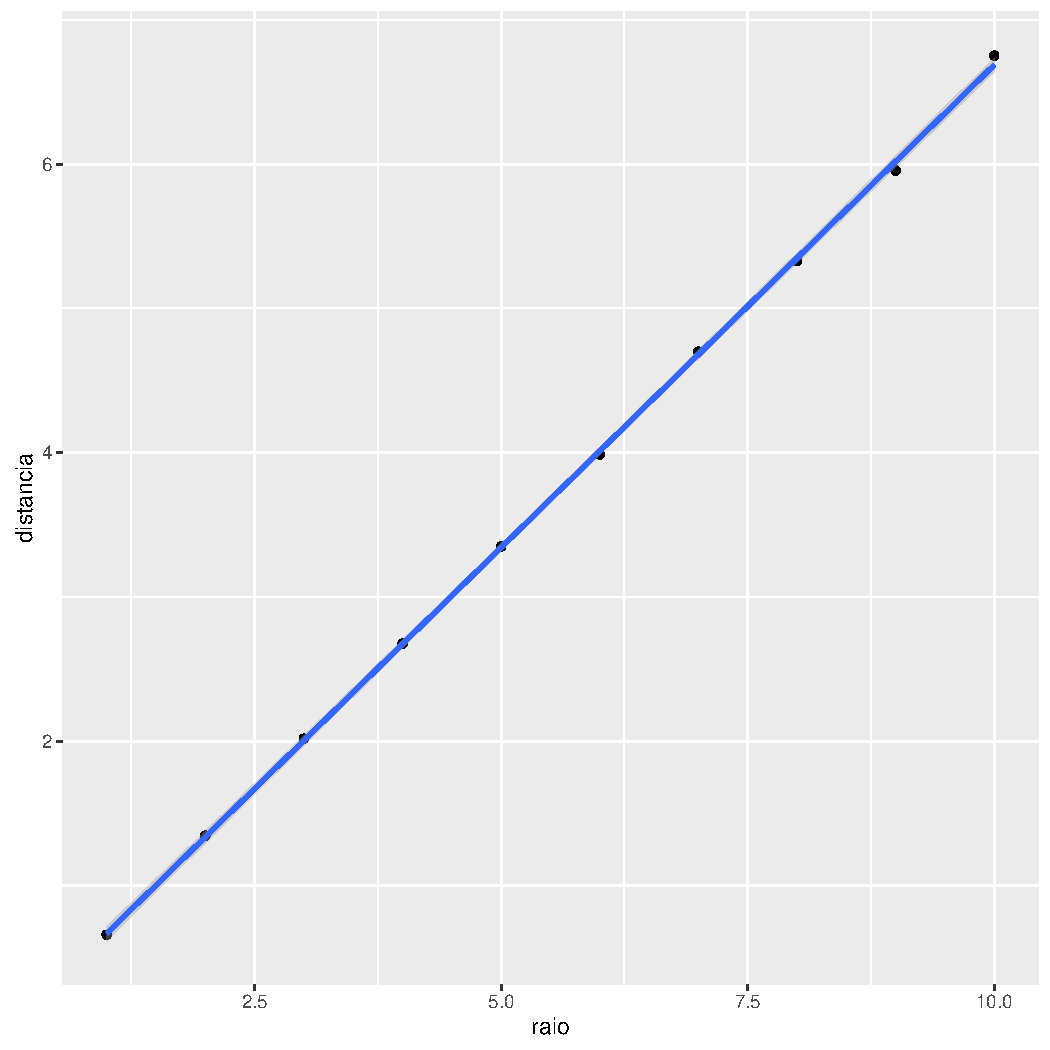
\includegraphics[scale=0.3]{chapter-computing-circle-distance}
 \caption{Variação linear da distância ao centro de
 acordo com o raio (\cref{ex:circle-rejection-2}).}
 \label{fig:circle-rejection-2}
\end{figure}
}{}

\begin{exercise}
 \label{ex:rejection-beta-a-b}
 Escreva código para
 simular de uma $\text{Beta}(a,b)$
 a partir de uma $\text{Uniforme}(0,1)$.
 Estime a média da $\text{Beta}(a,b)$ pelo
 método de Monte Carlo.
 Compare as taxas de rejeição do algoritmo proposto
 para alguns valores de $a$ e de $b$.
 Qual é a relação entre esses valores e
 a eficiência computacional do algoritmo proposto?
\end{exercise}

\cprotect \solution{\textbf{Solução}:
 O problema determina que
 $h(\theta) = \I(0 \leq \theta \leq 1)$.
 Podemos tomar $f(\theta) = \tilde{f}(\theta) = dbeta(\theta,a,b)$.
 Note que a moda da Beta$(a,b)$ é
 $\frac{a-1}{a+b-2}$. Portanto,
 $\tilde{f}(\theta) \leq \tilde{f}\left(\frac{a-1}{a+b-2}\right)h(\theta)$.
 Assim, as condições na amostragem por rejeição
 estão satisfeitas tomando
 $M= \tilde{f}\left(\frac{a-1}{a+b-2}\right)$.
 Portanto, podemos simular da Beta$(a,b)$ da
 seguinte forma
 \begin{lstlisting}[language=R]
simula_beta_rejeicao <- function(B,alpha,beta)
{
 M <- dbeta((alpha-1)/(alpha+beta-2),alpha,beta)
 amostra <- vector(mode="list", length=B)
 for(ii in 1:B)
 {
  T <- runif(1,0,1)
	rejeicoes <- 0
  while(runif(1,0,1) > dbeta(T,alpha,beta)/M) 
	{
	 T <- runif(1,0,1)
   rejeicoes <- rejeicoes+1
	}
	amostra[[ii]] <- c(T, rejeicoes)
 }
 return(amostra)
}
 \end{lstlisting} 

 Para entender de que forma o número de rejeições se
 comporta de acordo com $a$ e $b$, 
 geraremos amostradores para os casos em que $a=b$,
 para diversos valores de $a$ entre $2$ e $10$.
 O código está exibido abaixo.

 \begin{lstlisting}[language=R]
rejeicoes <- function(x) x[2]
param <- 2:10 
estimadores <- rep(NA, length(param))
for(ii in 1:length(param))
{
 estimadores[ii] <- monte_carlo(simula_beta_rejeicao, 10^4, rejeicoes, 
                                param[ii], param[ii])[["estimador"]]
}
dados <- data.frame(parametros=param, rejeicoes=estimadores)
ggplot(data=dados, aes(x=parametros, y=rejeicoes))+
geom_point()+
geom_smooth(method='lm',formula=y~x)
 \end{lstlisting}

 \begin{figure}
  \centering
  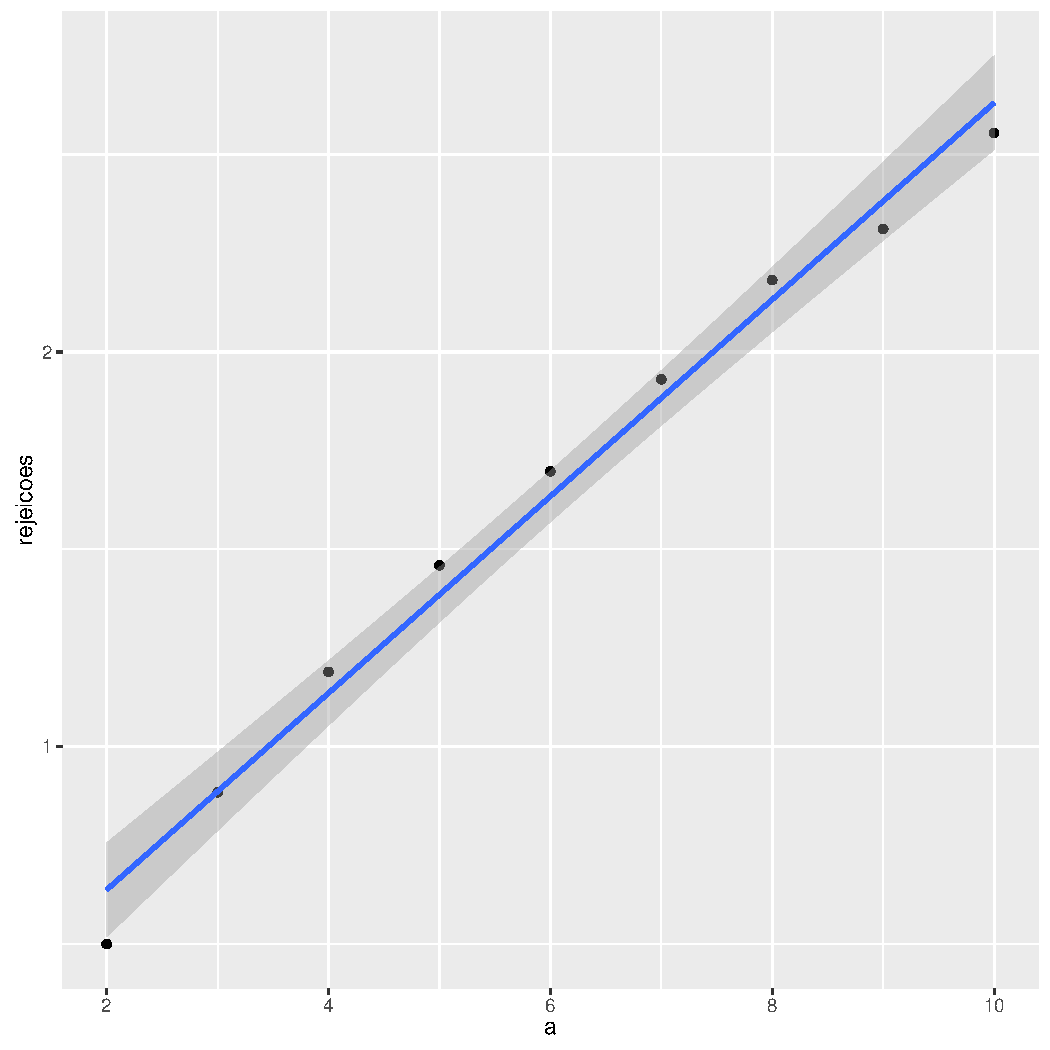
\includegraphics[scale=0.3]{chapter-computing-beta-rejections}
  \caption{Variação da taxa de rejeição
  de acordo com o valor de $a$
  (\cref{ex:rejection-beta-a-b}).}
  \label{fig:rejection-beta-a-b-1}
 \end{figure}

 A \cref{fig:rejection-beta-a-b-1} mostra que,
 quanto maiores os valores de $a$ e $b$, 
 maior a taxa de rejeição. 
 Isto ocorre pois a distribuição da Beta(a,b) 
 fica mais ``diferente'' da distribuição Uniforme(0,1)
 à medida que o valor de $a$ e $b$ aumentam.
 Este fato é ilustrado na
 \cref{fig:rejection-beta-a-b-2}.

 \begin{figure}
  \centering
  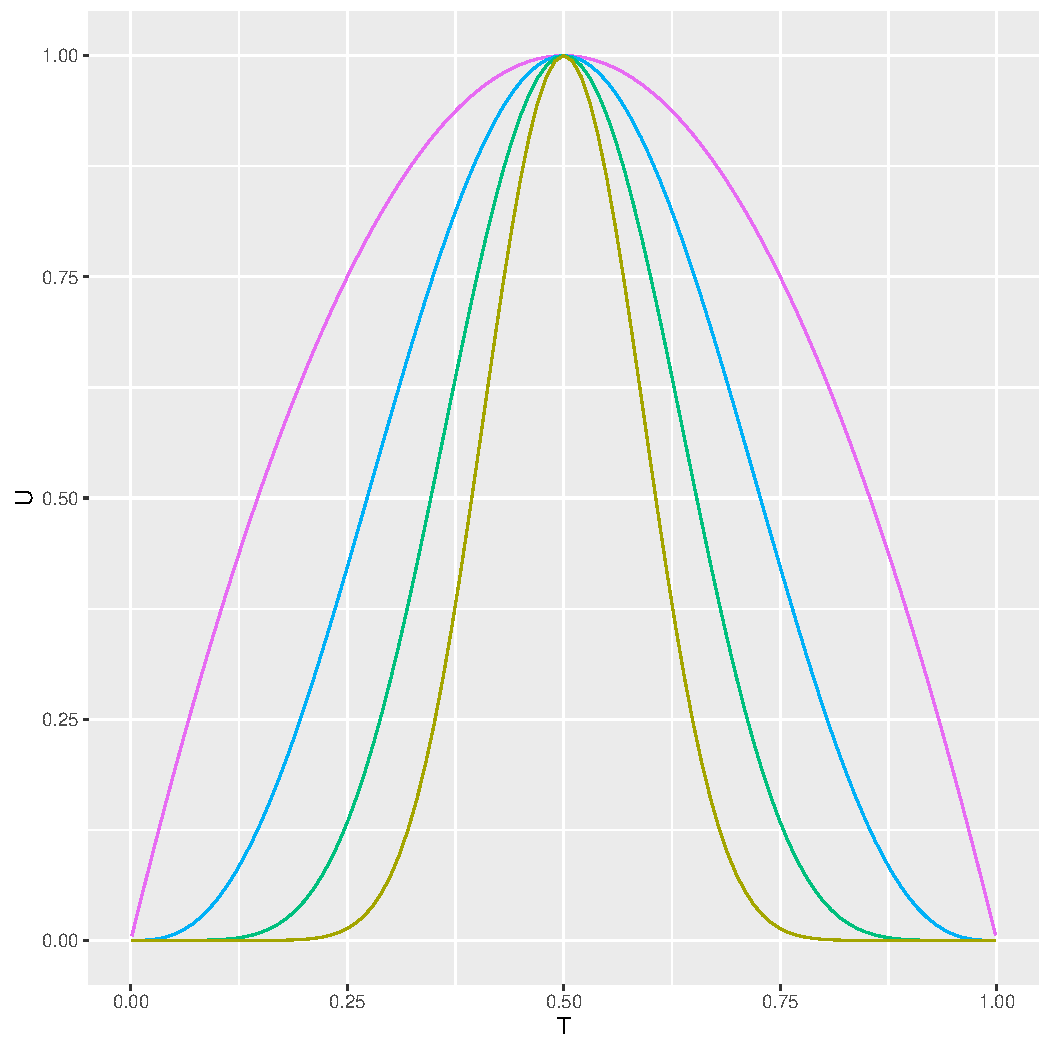
\includegraphics[scale=0.5]{chapter-computing-rejection-beta-a-b}
  \caption{Ilustração das regiões de rejeição
  para a Beta(2,2) (roxo), a Beta(4,4) (azul),
  a Beta(8,8) (verde) e a Beta(16,16) (marrom).}
  \label{fig:rejection-beta-a-b-2}
 \end{figure}
}{}

\begin{exercise}
 Sob quais condições é possível usar
 o método da rejeição para simular de
 uma $\text{Beta}(a,b)$ a partir de uma
 $\text{Beta}(a^{*},b^{*})$?
\end{exercise}

\cprotect \solution{\textbf{Solução}:
 Se $f(\theta) = dbeta(a,b)$ e
 $h(\theta) = dbeta(a^{*},b^{*})$, então
 \begin{align*}
  \frac{f(\theta)}{h(\theta)}
  &= \frac{Beta^{-1}(a,b)\theta^{a-1}(1-\theta)^{b-1}}{Beta^{-1}(a^{*},b^{*})\theta^{a^{*}-1}(1-\theta)^{b^{*}-1}} \\
  &= \frac{Beta(a^{*},b^{*})}
  {Beta(a,b)} \theta^{a-a^{*}}(1-\theta)^{b-b^{*}}
 \end{align*}
 Note que, se $a < a^{*}$, então
 $\frac{f(\theta)}{h(\theta)}$ pode ser
 arbitrariamente grande tomando-se $\theta \approx 0$.
 Similarmente, se $b < b^{*}$, então
 $\frac{f(\theta)}{h(\theta)}$ pode ser
 arbitrariamente grande tomando-se $\theta \approx 1$.
 Nestes casos, não existe $M$ tal que
 $f(\theta) \leq Mh(\theta)$.
 Portanto, se $a< a^{*}$ ou $b < b^{*}$,
 então não é possível amostrar de uma Beta$(a,b)$ 
 a partir de uma Beta$(a^{*},b^{*})$.

 Contudo, se $a>a^{*}$ e $b>b^{*}$,
 então $\frac{f(\theta)}{h(\theta)}$ é
 proporcional à densidade de uma
 Beta$(a-a^{*}+1,b-b^{*}+1)$.
 Portanto, $\frac{f(\theta)}{h(\theta)}$ tem
 seu valor maximizado em
 $\theta = \frac{a-a^{*}}{a-a^{*}+b-b^{*}}$.
 Assim, obtemos,
 \begin{align*}
  \frac{f(\theta)}{h(\theta)}
  &\leq \frac{Beta(a^{*},b^{*})}{Beta(a,b)} \left(\frac{a-a^{*}}{a-a^{*}+b-b^{*}}\right)^{a-a^{*}}\left(1-\frac{a-a^{*}}{a-a^{*}+b-b^{*}}\right)^{b-b^{*}} \\
  f(\theta) &\leq \frac{Beta(a^{*},b^{*})}{Beta(a,b)} \left(\frac{a-a^{*}}{a-a^{*}+b-b^{*}}\right)^{a-a^{*}}\left(1-\frac{a-a^{*}}{a-a^{*}+b-b^{*}}\right)^{b-b^{*}} h(\theta)
 \end{align*}
 Portanto, podemos tomar $\tilde{f}(\theta)=f(\theta)$ e
 $M=\frac{Beta(a^{*},b^{*})}{Beta(a,b)} \left(\frac{a-a^{*}}{a-a^{*}+b-b^{*}}\right)^{a-a^{*}}\left(1-\frac{a-a^{*}}{a-a^{*}+b-b^{*}}\right)^{b-b^{*}}$.
 
 Assim, obtemos o código:

 \begin{lstlisting}[language=R]
# retorna uma beta(a1, b1) pelo metodo da rejeicao
# por meio de uma beta(a2,b2)
simula_beta_via_beta <- function(B,a1,b1,a2,b2) {
 M <- ((a1-a2)/(a1-a2+b1-b2))^(a1-a2)*(1-(a1-a2)/(a1-a2+b1-b2))^(b1-b2)
 amostra <- vector(mode="list", length=B)
 for(ii in 1:B) {
  T <- rbeta(1,a2,b2)
  while(runif(1) > T^(a1-a2)*(1-T)^(b1-b2)/M)  T <- rbeta(1,a2,b2)
  amostra[[ii]] <- T
 }
 return(amostra)
}
 \end{lstlisting}
}{}

\begin{exercise}
 Sob quais condições é possível usar
 o método da rejeição para simular de uma
 $\text{Gama}(a,b)$ a partir de uma
 $\text{Exponencial}(c)$? Escreva o
 código para realizar esta simulação. 
\end{exercise}


\include{chapters/09-2-computing-mcmc}
\include{chapters/10-review-3}

\include{chapters/11-test}

\bibliographystyle{apalike}
\bibliography{chapters/booklet}

\end{document}

